%These 
\documentclass[a4paper, 12pt]{report}
%--------------------------------------------------------------------------------------------------
\usepackage[utf8]{inputenc}
\usepackage[arabic, english, french]{babel}   							
\usepackage{arabtex}
\usepackage[T1]{fontenc}                             							
\usepackage{ragged2e} 			
\usepackage{threeparttable,booktabs,multirow,lscape}
\usepackage[letterpaper,margin=1in]{geometry} 
\usepackage[backend=bibtex, style=alphabetic]{biblatex} 					
\usepackage{rotating}
\usepackage[ruled,vlined,french]{algorithm2e}
\usepackage{graphicx}                    								
\usepackage{pdflscape}
\usepackage{afterpage}
\usepackage{capt-of}										
\usepackage{xcolor}
\usepackage{fancyvrb}    										
\usepackage[colorlinks=true,linkcolor=blue, citecolor=blue]{hyperref}
\usepackage{setspace}
%
\addbibresource{21_Bibliographie.bib} 
\graphicspath{ {data/} } 
%------------------------------------------------------------------------------------------------------
\usepackage{amsfonts}
\usepackage{amssymb}
\usepackage{amsmath}
\usepackage{amsthm}
\usepackage{mathrsfs}

\geometry{ a4paper, total={170mm,257mm}, left=25mm, top=25mm, }
%------------------------------------------------------------------------------------------------------
\setlength{\parindent}{4em}
\setlength{\parskip}{0.5em}     
\renewcommand{\baselinestretch}{1} 
%------------------------------------------------------------------------------------------------------
\usepackage[framemethod=TikZ]{mdframed}
\usepackage{calc}
%
\newcommand{\definebox}[2]{
    \newcounter{#1}
    \newenvironment{#1}[1][]{
        \stepcounter{#1}
        \mdfsetup{
            frametitle={
                \tikz[]
                \node[rectangle,fill=white]{\strut \MakeUppercase#1~\csname the #1\endcsname\ifstrempty{##1}{}{:~##1}};
            }
        }
        \mdfsetup{innertopmargin=1pt, linecolor=#2, linewidth=1pt,topline=true, frametitleaboveskip={\dimexpr (\ht\strutbox)*-1\relax},}   %
        \begin{mdframed}[]\relax
        }
       {\end{mdframed}}
}
%------------------------------------------------------------------------------------------------------
\definebox{définition}{}

%------------------------------------------------------------------------------------------------------
\begin{document}
	% - - - - - - - début de la page 
\thispagestyle{empty}     %\includegraphics[scale=0.12]{upmc-logo.png}
\begin{center}

\includegraphics[scale=0.9]{uoran001}
\end{center}

{\large
 \vspace*{1cm}

\begin{center}
{\bf TH\'ESE}\\                                 		\vspace*{0.5cm}
Pour l'obtention du\\
{\bf Diplome de Doctorat en Sciences} \ \\   	\vspace*{1cm}
{\Large {\bf INFORMATIQUE}}\\                     	\vspace*{1cm}
\end{center}

\begin{center}					%\flushleft{Sujet de la th\`ese :}\ \\   \ \\
{\Large {\bf Ordonnancement d'un DAG avec transfert des données sur une plateforme NUMA multicore \\ }}
\end{center}

 \begin{center}
Pr\'esent\'ee par \ \\                                      	\vspace*{0.25cm}
{\Large {\bf Slimane Mohammed}}\\             	\vspace*{1cm}
\end{center}

\vspace*{1cm} 
%\flushleft{soutenue le 30 Juin 2018 inchaallah}\\[1ex]
\flushleft{soutenue devant le jury composé de :  }\\[1ex]
\flushleft{\begin{tabular}{r@{\ }l l l}
& Mr. Kadour Mejdi                   & Professeur, Univ. Oran1  & Président \\
& Mr. Sekhri Larbi                   & Professeur, Univ. Oran1 & Directeur de thèse\\
& Mr. Benmohamed Mohamed   & Professeur, Univ. Constantine 2  & Examinateur \\
& Mr. Allaoua Chaoui               & Professeur, Univ. Constantine 2  & Examinateur \\
& Mr. Djebbar  Bachir              & Professeur, USTOMB & Examinateur \\
& Mme.Taghezout Noria             & MCA, Univ. Oran1 & Examinatrice
\end{tabular}}
}
% - - - - - - - fin de la page  \thispagestyle{empty}
	%\section*{Remerciement}
\newpage
\begin{center}

\includegraphics[scale=0.3]{bismi001}
\end{center}

\begin{otherlanguage}{arabic}


%\section*{تاريخ}
\section*{}
\centering
{\large
يرفع الله الذين آمنوا منكم والذين أوتوا العلم درجات
\\



صدق الله العظيم
}


%بسم الله الرحمن الرحيم\\
%(يَرْفَع*ِ الله*ُ الَّذِين*َ آمَنُوا مِنكُم*ْ وَ الَّذِين*َ أُوتُوا اْلعِلْم*َ دَرَجَات*ٍ)\\ % for example I want to change font and size for this line
%صَدَق*َ الله*ُ الْعَلِي*ُ الْعَظِيْم*ُ\\%

%(يَرْفَع*ِ الله*ُ الَّذِين*َ آمَنُوا مِنكُم*ْ وَ الَّذِين*َ أُوتُوا اْلعِلْم*َ دَرَجَات*ٍ)\\ % for example I want to change font and size for this line
%صَدَق*َ الله*ُ الْعَلِي*ُ الْعَظِيْم*ُ\\
%
%
%\thol
%بِسْم*ِ الله*ِ الرَّحْمن*ِ الرَّحيم*ِ\\
%بسم الله الرحمن الرحيم\\
%(يَرْفَع*ِ الله*ُ الَّذِين*َ آمَنُوا مِنكُم*ْ وَ الَّذِين*َ أُوتُوا اْلعِلْم*َ دَرَجَات*ٍ)\\ % for example I want to change font and size for this line
%صَدَق*َ الله*ُ الْعَلِي*ُ الْعَظِيْم*ُ\\
\end{otherlanguage}      	     \thispagestyle{empty}
	\newpage
\begin{otherlanguage}{arabic}
\section*{}
\begin{center}
%\centering
{\large
اهداء \\ 
\vspace{50mm}
الي كل الاحبة الذين كانوا معنا ثم رحلوا \\
الي روح ابي و امي \\
الي روح اختي الصغرى \\
الي كل مرضى السرطان الذين يعانون ولايجدون من يخفف الامهم \\
اهدي هذا العمل
}
\end{center}
\end{otherlanguage}
     	\thispagestyle{empty}
	\selectlanguage{english} 


\begin{abstract}

\begin{center}					%\flushleft{Sujet de la th\`ese :}\ \\   \ \\
{\large {\bf Scheduling of DAG with data placement on multicore NUMA platform\\ }}
\end{center}

%\justify
Directed acyclic graphs (DAG) based scheduling algorithms in traditional computing paradigms focus more on computational tasks and less than on the data placement during scheduling mapping. In the hierarchical memories context, this behavior will have negative impact on performance of system. With the introduction of non-uniform memory access (NUMA) multicore architectures, simultaneous optimization of computation and data placement in DAG based scheduling and mapping become the most challenging topics in scheduling related research. Such architecture exposes multilevel hierarchical memories with different characteristics which make the cost of the communication different in each level. From the other side, some interdependent tasks are communication intensive tasks that need to load and store their data frequently from the memory depending on data location, the performance of such system and its scheduler depends not only on its threads scheduling decision but also on its data locality decision (the mapping of the thread data).

In this thesis, we tackle the problem of the scheduling parallel applications described by DAG in target platforms by exploring case where not just computation and communication are considered in scheduling decision but also data placement on hierarchical memories platforms. The current scheduling and mapping policies try to reduce the overall penalties of the remote access by taking into account the data locality in the scheduling decisions. But most of the work done is for independent tasks context with static initialization. To do this for DAG application execution on the hierarchical platforms, it is necessary to find a way to combine both policies to get the most appropriate decision about when and where to schedule thread and where to place its data. 
In this work, we will: 

\begin{enumerate}
\item Include the platform topology information (supplied by run-time environment at start time of application).
\item Use the application pattern (application structure provided by developers).
\item Divide the tasks set to a number of disjoint sets based on this structure and on task state.
\item Wide the tasks visibility by exploring a large horizon in order to gather more information about the state of current process running DAG.
\item Balance the load using distance based work stealing strategy at run-time.
\end{enumerate}

These are the main ideas of the proposed scheduling and mapping policy of this work integrated as heuristics in this process to guide it and to reduce the impact of NUMA penalties on the completion total time of the DAG and preserve the system performance.

\textbf{Key words} : Task graph, DAG based scheduling, mapping, data locality, Multicore machines, NUMA architectures, Hierarchical platforms, Execution Horizon, Work stealing, Load balancing.

%\justify
\end{abstract}

\newpage
\selectlanguage{french} 
\begin{abstract}

\begin{center}					%\flushleft{Sujet de la th\`ese :}\ \\   \ \\
{\large {\bf Ordonnancement d'un DAG avec transfert des données sur une plateforme NUMA multicore \\ }}
\end{center}

Les algorithmes d'ordonnancement des graphes de tâches (DAG) selon l’approche classique se concentrent davantage sur les tâches de calcul et leurs dépendances ( communi-cation ) et donnent moins d’importance au placement des données lors de l'allocation. Dans le contexte des plateformes hiérarchiques, ne pas placer les données des threads de façon appropriée impacte les performances du système. Avec l'introduction des architectures d'accès non uniforme à la mémoire (NUMA), l'optimisation simultanée du placement des threads et des données d’un DAG est devenue cruciale. Une telle architecture possede un système de mémoire hiérarchique multi niveaux avec des caractéristiques différentes qui rend le coût de la communication différent dans chaque niveau. Une bonne partie du temps des tâches dépendantes orientées données se consomme en chargeant ou sauvegardant ses données de la mémoire en fonction du placement initial. Les performances d’un tel système et son ordonnanceur dépendent non seulement de sa décision d’affectation des threads mais aussi de sa décision du placement des données.

Dans cette thèse, nous abordons le problème de l'ordonnancement d'applications parallèles décrites par un DAG sur la plateforme cible en explorant le cas où non seulement le calcul et la communication sont considérés, mais aussi le placement de données sur les plateformes hiérarchiques. Les politiques courantes de l’ordonnancement et l'allocation de la mémoire tentent d’atténuer l’effet NUMA en réduisant la pénalité d’accès distant à la mémoire en tenant en compte la localité des données lors de la décision de l’ordonnancement. Ce travail propose  de :

\begin{enumerate}
\item Inclure l’information sur la topologie (fournie par l’environnement runtime au début de l’exécution de l’application) de la plateforme.
\item Utiliser le motif de l’application (sa classe information fournie par le développeur de l’application) à exécuter.
\item Regrouper les tâches dans des classes disjointes en se basant sur cette structure et l'état de la tâche.
\item Elargir le champs de visibilité des tâches en explorant un large horizon afin de collecter plus d'informations sur l'état courant du processus d'éxecution de DAG.
\item Equilibrer la charge au temps d’exécution en utilisant la stratégie de vol de travail basée sur la distance.
\end{enumerate}

Comme idées de bases, ces propositions seront integrées comme heuristiques dans la politique de l’ordonnancement des threads et le placement des données pour guider ce processus et l'aider à réduire l’effet NUMA sur le temps total d’exécution d’un DAG et de préserver les performances du système.

%\justify
\textbf{Mots-clés} : Graphe de tâches, Ordonnancement DAG, Placement, Localité de données, Machines multicœurs, Architectures NUMA, Caches hiérarchiques, Horizon d'éxecution, Vol de travail, Equilibrage de charge.
%\justify
\end{abstract}    	     \thispagestyle{empty}
	%\section*{Remerciement}
\newpage
\begin{otherlanguage}{arabic}   %\section*{تاريخ}
\begin{abstract}
\justify
\begin{center}
جدولة \textLR{DAG} مع تموضع المعطيات على بنية  \textLR{NUMA}  المتعددة النواة
\end{center}

خورزميات الجدولة القائمة على المخططات الموجهة اللاحلقية  \textLR{DAG} المستعملة في اطار الحوسبة التقليدية تصب جل تركيزها على المهمات الحسابية اكثر من تموضع المعطيات خلال عملية الجدولة و التموضع.
في سياق الذاكرات المتسلسلة الترتيب, هذا النمط يكون له اثر سلبي على اداء و فعالية النظام ككل.
مع استحداث البنى المتعددة النواة و ذات ذاكرة لا متماثلة و غير متناظرة الولوج (\textLR{NUMA}) فان ايجاد الجدولة-الحل و التموضع الامثلين في ان واحد لمسألة جدولة و تموضع مخطط \textLR{DAG} يعد من الامور المستعصية التي تشكل تحديا في ادبيات البحث العلمي الخاص بمسائل الجدولة.
بنى كهذه تعرض ذكرات متسلسلة الترتيب و متعددة المستويات بخصائص مختلفة, الامر الذي يجعل تكلفة الاتصال متباينة في كل مستوى من جهة و من جهة اخرى بعض المهام المترابطة لها جانب اتصلي معتبر غالبا ما تحمل و تحفظ معطياتها من و الى الذاكرة مرارا متعلقة بتموضع هذه الاخيرة.
اداء هذا النظام و أداة الجدولة لا يعتمد فقط على جدولة عمليات التنفيذ المخففة و لكن ايضا على قرار التموضع الخاص بمعطياتها.

في هذه الاطروحة نسعى الى حل مسألة جدولة التطبيقات المتوازية المعبر عنها بـ \textLR{DAG} على البنى المستهدفة و ذلك من خلال استكشاف الحالة التي ليس فقط الحوسبة و الاتصال يأخذان بعين الاعتبار خلال اتخاذ قرار الجدولة و لكن ايضا تموضع المعطيات على ذكرات البنى اللامتناظرة. ان سياسات الجدولة و التموضع الحالية تسعى الى التقليل من حدة التأثير العام لمعوق الولوج البعيد بأخذها بالحسبان تموضع المعطيات في قرار الجدولة. 
   لكن معظم الابحاث السابقة كانت في سياق المهمات المستقلة. لتطبيق ذلك على تنفيذ التطبيقات المعبر عنها بـ \textLR{DAG} على البنى المتسلسلة الترتيب, من الضروري ايجاد سبيل للمزج بين كلتا السياستين للتوصل الى القرار الانسب حول متى و اين  نجدول عمليات التنفيذ و اين نضع معطياتها.
   في هذا العمل, سوف نقوم بـ :
   \begin{enumerate}
\item ادراج معلومة طبولوجيا بنى التنفيذ (المقدمة من بيئة مرحلة التنفيذ خلال بدء التطبيق).
\item استخدام نمط التطبيق(بنية التطبيق معطاة من طرف المبرمج).
\item بناءا على هذه البنية و حالة المهمات, سوف نجزء مجموعة المهمات على عدد من المجموعات المنفصلة.
\item توسيع مجال رؤية المهمات باستكشاف افق اوسع و ذلك لجمع معلومات اكثر حول الحالة الراهنة لعملية تنفيذ \textLR{DAG}.
\item حفظ توازن العبء على البنية باستخدام استراتيجية سرقة العمل  خلال مرحلة التنفيذ القائمة على المسافة 
\end{enumerate}
    
هذه هي الافكار الرئيسية المقترحة لسياسات الجدولة و التموضع لهذا العمل المدرجة كأرستيكس في هذه العملية لارشادها و للتقليل من اثر المعوقات  على زمن الانتهاء الكلي و لحفظ اداء النظام.

\textbf{كلمات-مفتاح} :  
مخطط المهام, جدولة \textLR{DAG}, تموضع المعطيات, جوارية المعطيات, حواسيب بمعالج متعدد النواة, بنى \textLR{NUMA}, التخزين البيني المتدرج, أفق التنفيذ, سرقة العمل, توزيع العبء.
\justify
\end{abstract}
\end{otherlanguage}    	  	\thispagestyle{empty} 
	\newpage
\section*{Remerciement}

\begin{flushright}
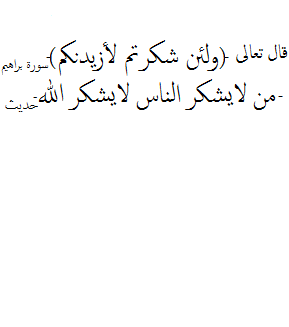
\includegraphics[scale=0.7]{remercie006}
\end{flushright}

\textit{Je remercie} \textbf{ALLAH} \textit{le tout puissant la source de toutes les grâces qui nous entourent de nous avoir donné la force et le courage à accomplir ce travail}.  

\textit{Je remercie mon directeur de thèse, le Professeur} \textbf{Sekhri Larbi} \textit{pour avoir accepté de superviser et diriger ce travail pendant ces années, pour sa contribution active dans l’accomplissement de ce travail, et pour ses conseils et son aide. Son expérience, ses critiques et ses encouragements ont été très bénéfiques et surtout sa patience de m'avoir encadré}. 

\textit{Je tiens tout d’abord à remercier le Professeur} \textbf{Kadour Mejdi} \textit{pour l’honneur qu’il me fait en acceptant de présider le jury de cette thèse}. 

\textit{J'exprime toute ma gratitude aux professeurs} \textbf{Benmohamed Mohamed, Allaoua Chaoui et Djebbar  Bachir} \textit{, le Docteur } \textbf{Taghezout Noria} \textit{pour avoir consacré de leur temps pour la lecture de ce manuscrit. Je leur suis vivement reconnaissant d’avoir accepté de participer au jury}.

\textit{Je dis aussi un grand merci à ma femme qui s’est fortement impliquée dans les aspects, pas toujours agréables, de correction des fautes d’orthographe et de la logistique de cette thèse. Ainsi que ma sœur, mes deux frères et mes amis pour le soutien, l'encouragement et l'aide si nécéssaire pour accomplir un tel travail.}

\textit{A Vous tous, Que vous trouverez ici mes remerciements et ma gratitude les plus profonds.}
 	\thispagestyle{empty}
%
	\begin{spacing}{0.04}
	\tableofcontents 				\thispagestyle{empty}
	\listoffigures 					\thispagestyle{empty}
	\listoftables 					\thispagestyle{empty}
	\listofalgorithms 				\thispagestyle{empty}
	\newpage
\section*{Liste des Abréviations}

\noindent \\
\begin{tabular}{ l l l }
\textbf{Abrev} 	& \textbf{English}						&	\textbf{Français} \\[1.0ex]
\textbf{AoXT}  	& Affinity on First Next Touch  		& 	Affinité d'acces Premiere fois Suivant \\[0.6ex]
\textbf{BC}  		& Cache Bloc 							& 	Bloc Cache \\[0.6ex]
\textbf{BM}  		& Memory Bloc 							& 	Bloc Mémoire \\[0.6ex]
\textbf{CPU}  	& Central Processing Unit (processor)	& 	Unité centrale du traitement (processeur) \\[0.6ex]
\textbf{DAG }  	& Direct acyclic graph 					& 	Graphe acyclique derigé  \\[0.6ex]
\textbf{DRAM }  & Dynamic Random Access Memory      & Mémoire à acces aleatoire dynamique \\[0.6ex]
\textbf{FBoPP } 	& FeedBack oriented Page Placement & Retroaction orientée placement de Page \\[0.6ex]
\textbf{FP }  		& Fireplane interconnect SunMS & Fireplane interconnect SunMS \\[0.6ex]
\textbf{HLSMN} 	& High Level Simulator of MC NUMA & Simulateur de Haut niveau MC NUMA \\[0.6ex]
\textbf{HT }  	& HyperTransport (AMD) & HyperTransport (AMD) \\[0.6ex]
\textbf{ICN }  	& InterConnect Network & Réseau D'interConnexion \\[0.6ex]
\textbf{ILP}  		& Instruction Level Parallelism & Parallelisme au niveau des instructions \\[0.6ex]
\textbf{IMC }  	& Integrated Memory Controller  & Controlleur Mémoire integré \\[0.6ex]
\textbf{JIT}  		& Just In Time (Compiler) & Juste au temps (Compilateur) \\[0.6ex]
\textbf{L1/2/3}  	& L1/2/3 Cache (Level 1/2/3) & Cache Niveau 1/2/3 \\[0.6ex]
\textbf{LAWS }  	& Locality-Aware Work-Stealing  & Vol de travail basé sur la Localité \\[0.6ex]
\textbf{LFU}  	& Least Frequently used & Moins Utilisé Fréquement  \\[0.6ex]
\textbf{LRU}  	& Least Recently used & Moins Utilisé Récement  \\[0.6ex]
\textbf{MAI }  	& Memory Affinity Interface & Interface d'Affiity Mémoire \\[0.6ex]
\textbf{MC }  	& MultiCore Processor  & Processeur Multcoeurs \\[0.6ex]
\textbf{MIMD}  	& Multiple Instructions Multiple Data  & Plusieurs Instructions Plusieurs données \\[0.6ex]
\textbf{MINAS} 	& Memory Affinity Management FW & Framework de Gestion Affinité Mémoire \\[0.6ex]
\textbf{MISD}  	& Multiple Instructions Single Data  & Plusieurs Instructions Une seule donnée\\[0.6ex]
\textbf{MPO }  	& Memory Placement Optimisation & Optimisation du Placement Mémoire\\[0.6ex]
\textbf{MRV}  	& Most Recent Value & Valeur la plus recente \\[0.6ex]
\textbf{MSNoC}	& MultiSocket Network on Chip & MultiSocket réseau sur Puce \\[0.6ex]
\textbf{NUMA}  	& Non Uniform Memory Architecture  & Architecture à Mémoire non uniforme \\[0.6ex]
\textbf{QPI}  	& Quick Path Interconnect (Intel) & Quick Path Interconnect (Intel) \\[0.6ex]
\textbf{SDN }  	& SubDagNode & Noeud d'un sous DAG \\[0.6ex]
\textbf{SIMD}  	& Single Instruction Multiple Data  & Un Flux d'Instructions données multiples\\[0.6ex]
\textbf{SIMD}  	& Single Instruction Multiple Data  & Un Flux d'Instructions Une seule données\\[0.6ex]
\textbf{SMP}  	& Symetric MultiProcessors & Multiprocesseurs Symmetrique \\[0.6ex]
\textbf{SMT}  	& Simultaneous MultiThreading  & MultiThreading Simultané \\[0.6ex]
\textbf{SRAM}  	& Static Random Access Memory      & Mémoire à acces aleatoire statique \\[0.6ex]
\textbf{UMA}  	& Uniform Memory Architecture  & Architecture à Mémoire uniforme \\[0.6ex]
\textbf{WP }  	& Write Policy & Politique de Modification \\[0.6ex]
\textbf{WS }  	& Work Stealing (LoadBalancing) & Vol de travail (Equilibtrage de charge) \\[0.6ex]
\textbf{XH-VHFU}  & eXecution Horizon Heuristic  & Heuristique Horizon d'execution
 \end{tabular}

  	\thispagestyle{empty}
	\end{spacing}
%
	\clearpage
	\pagenumbering{arabic}
	\chapter{Introduction} 
\justify \hspace{\parindent}
Au début des années deux mille, l'industrie des \textbf{microprocesseurs} a atteint sa limite avec sa version initiale des \textbf{monoprocesseurs} en se heurtant aux 3 murs qui ont freiné la \textbf{loi de Moore} \cite{moor65} après 50 ans de prédiction.
%
Par conséquent, l'industrie a opté pour des \textbf{architectures multicœurs} intégrant plusieurs \textbf{cœurs} (core ou unités de calcul) sur une même puce où chaque cœur dispose de sa propre \textbf{mémoire cache} ou partagée avec les autres cœurs, d'une \textbf{mémoire principale} commune constituée de plusieurs bancs de mémoires 
le tout par son organisation physique forme une \textbf{hiérarchie de mémoire} de plusieurs niveaux, 
ainsi le système dispose de suffisamment de ressources pour traiter en parallèle les \textbf{applications multitâches}. 
%
L’évolution de l'informatique a pris une autre direction plus spectaculaire, une autre aventure commence l'informatique parallèle grand publique ou le coût des ressources de calcul devient abordable et l'exécution parallèle des applications n'est plus un luxe (s'est démocratisée). 
%
Cette évolution n'était pas suivie par une conception des \textbf{modèles de programmation parallèle} et des outils logiciels adaptés à ces ressources (les systèmes de hautes performances d'aujourd'hui sont composés de centaines de cœurs et les systèmes futurs en intègreront des milliers - systèmes massivement parallèles).
%
Les architectures parallèles récentes ne cessent pas de se complexifier, des \textbf{plateformes multicœurs multi-socket} intégrant plusieurs nœuds de calcul sur une même carte mère ou puce (multicœurs multisocket or multisocket Network on Chip MSNoC) \cite{msoc00} ont été conçues comme solution aux \textbf{problèmes du bus  partagé} (congestion) dans les \textbf{architectures symétriques (SMP)} \cite{qaca17}.  
Afin de fournir une \textbf{bande passante} mémoire suffisante dans ces systèmes, la mémoire vive est distribuée physiquement sur plusieurs \textbf{contrôleurs mémoire} associe à un \textbf{nœud} avec un \textbf{accès non-uniforme à la mémoire (NUMA)} \cite{qaca17}. 

\section{Problématique et motivation} %
\justify \hspace{\parindent}
En raison de la complexité de ce dernier type d'architectures parallèles, les \textbf{coûts d'accès mémoire} peuvent varier en fonction de la distance entre le processeur et le banc mémoire accédé. 
%
Ce fait a introduit une \textbf{pénalité} sur le \textbf{temps d'exécution total} des \textbf{applications parallèles} qui s'exécutent sur les nœuds de cette plateforme \cite{qaca17}. 
%
D'un autre coté, vu que le nombre de cœurs est devenu très élevé dans les  architectures modernes (manycore), telles machines entraînant des accès mémoire concurrents qui conduisent à des ponts chauds sur des bancs mémoire, générant des \textbf{problèmes d'équilibrage de charge}, de \textbf{contention mémoire} et d'\textbf{accès distants} \cite{qaca17}.   
%
Des travaux de recherche récents ont identifié les \textbf{modèles de programmation} à base de \textbf{tâches} indépendantes à \textbf{granularité} fine comme une approche clé pour exploiter la puissance de calcul des architectures généralistes massivement parallèles \cite{qaca17}. 

\justify \hspace{\parindent}
Toutefois, peu de recherches ont été conduites sur l'optimisation dynamique des programmes parallèles à base de \textbf{tâches dépendante} afin de réduire l'impact négatif sur les performances résultant de l'\textbf{effet NUMA}.

\justify \hspace{\parindent}
Les plates-formes multicœurs avec un accès mémoire non uniforme (MC-NUMA) sont devenues des ressources usuelles de \textbf{calcul haute performance}.

\justify \hspace{\parindent}
Par conséquent, les principaux défis sur les plates-formes NUMA pour \textbf{ordonnan-cer} une application parallèle décrite par un \textbf{graphe de tâches dépendantes acyclique (DAG)} sont :

\justify \hspace{\parindent}
1- \textit{Réaliser la bonne \textbf{allocation tâche/thread-nœud} (Trouver l'ordre optimal ou proche pour exécuter les tâches de ce DAG sur les nœuds de la plate-forme).}

\justify \hspace{\parindent}
2- \textit{Réaliser le bon \textbf{placement donnée-thread/mémoire-nœud} (Mapper les don-nées de telle façon de réduire la \textbf{latence des accès mémoire} et de maximiser la bande passante)}. 

\justify \hspace{\parindent}
3- \textit{\textbf{Equilibrer la charge} entre les cœurs/nœuds de calculs}.

\justify \hspace{\parindent}
4- \textit{Garder certaine \textbf{proximité spatiale et temporelle} entre les tâches dépendantes lors de l'exécution afin de préserver la \textbf{localité des données}}.

\section{Objectifs de la thèse} 
\justify \hspace{\parindent}
Le but de cette thèse est de :

\justify \hspace{\parindent}
1- \textit{Déterminer les enjeux et les opportunités concernant l'exploitation efficace de machines multicœurs NUMA par des applications parallèle à base de tâches dépendantes décrite par un DAG, en optimisant son ordonnancement}.

\justify \hspace{\parindent}
2- \textit{Proposer des mécanismes efficaces pour le placement de tâches et de données, améliorant la localité des accès à la mémoire ainsi que les performances systèmes, en optimisant le placement des données associes aux tâches}. 

\justify \hspace{\parindent}
Les décisions de placement sont basées sur l'exploitation des informations sur les dépendances entre tâches disponibles via des annotations et d'autre technique fournies par les langages de programmation parallèle à base de tâches et les \textbf{supports exécutifs modernes (runtime)}. 

\section{Contributions} 
\justify \hspace{\parindent}
Dans ce contexte, l'objectif principal de cette thèse est  d'assurer un ordonnancement efficace des tâches d'un DAG sur des machines NUMA multicœurs en contrôlant le placement des données associes aux tâches en exécutions en favorisant la proximité spatiale et temporelle (\textbf{affinité mémoire}). 

\justify \hspace{\parindent}
La contribution majeure de cette thèse consiste à concevoir une approche d'ordonnance-ment d'un DAG dans le contexte NUMA qui favorisent l'affinité mémoire tâche/donnée et la proximité de voisinage tâche/tâche en minimisant la métrique classique d'un problème d'ordonnancement qui est le temps total d'exécution des tâches. Nos contributions : 

\justify \hspace{\parindent}
1- \textit{Réalisation d'un \textbf{simulateur NUMA} dont les principaux aspects des plateformes NUMA ont été implémenté dans d’un simulateur que nous avons utilisé pour les évaluations présentées dans ce travail}.

\justify \hspace{\parindent}
2- \textit{Etude et comparaison de l'impact des politiques d'ordonnancement des tâches / placement des données sur les performances des applications sur les plateformes NUMA dont les tâches sont indépendantes (pas de communication ou partage des données entre les tâches)}.

\justify \hspace{\parindent}
3- \textit{Conception d'un algorithme d'ordonnancement basé sur l'heuristique \textbf{Horizon d'exécution adapté NUMA} qui consiste à partitionner l'ensemble des tâches en plusieurs classes disjointes en fonction de l'état courant d'exécution des tâches et sélectionner celle qui va élargir cet horizon}. 

\justify \hspace{\parindent}
4- \textit{\textbf{Equilibrage de charge} dynamique entre les nœud/cœurs de la plateforme en utilisant une stratégie de \textbf{vol de travail} adapté pour NUMA basé sur la \textbf{matrice distance} de la plateforme}. 

\section{Plan et Organisation de la thèse}
\justify \hspace{\parindent}
Ce document s’organise de la façon suivante : 

\justify \hspace{\parindent}
1- Le \textbf{présent chapitre} introduit le contexte, la motivation et la contribution de notre étude. 

\justify \hspace{\parindent}
2- Le \textbf{deuxième chapitre} est consacré à la présentation de l'évolution de la technologie des microprocesseurs, des architectures parallèles et en particulier SMP-UMA et la platefor-me NUMA. Nous exposons les concepts clés qui ont une relation directe sur l'exécution des applications parallèles.

\justify \hspace{\parindent}
3- Le \textbf{troisième chapitre} présente le modèle de la description des applications parallèles à base de tâches et en particulier le modèle du graphe de tâches (DAG) qui est le sujet de notre étude. La terminologie associée à ce contexte est expliquée dans cette partie en commençant par le processus de la description, ensuite le processus de l'exécution et à la fin les algorithmes utilisés.

\justify \hspace{\parindent}
4- Le \textbf{quatrième chapitre} présente l'état de l'art des algorithmes d'ordonnancement placement dans le contexte des Multicœurs et de NUMA en dressant un panorama des politiques d'ordonnancement/placement existants

\justify \hspace{\parindent}
5- Dans le \textbf{cinquième chapitre}, nous introduisons nos \textbf{heuristiques} pour améliorer les algorithmes existants d'ordonnancement NUMA et équilibrer la charge des supports exécutifs.

\justify \hspace{\parindent}
6- Le \textbf{sixième chapitre} est consacré à l'introduction du simulateur réalisé ainsi que la simulation des algorithmes  donnés dans le chapitre précédents suivi par une analyse des résultats des différents scenarios expérimentés.

\justify \hspace{\parindent}
7- Le \textbf{dernier chapitre} comme conclusion de ce travail, il récapitule nos principales contributions. Il présente également les pistes de recherche futures à explorer et l’extension de nos travaux à d’autres champs d’application (NUMA clusters ou autre).

%--------------------------------------------
\section{Production scientifique} 
\justify \hspace{\parindent}
Ce travail a mené à la \textbf{publication} deux articles acceptés dans les revues EEA  et IJIST ainsi qu’une version initiale présentée dans la conférence LAPECI.

\begin{itemize}
  \item Mohamed Slimane et Larbi Sekhri. Modeling the Scheduling Problem of Identi-cal Parallel Machines with Load Balancing by Time Petri Nets. In, International Journal of Intelligent Systems Technologies and Applications, déc. 2014, p. 42-48. \cite{slim1214}

  \item Mohamed SLIMANE et Larbi SEKHRI. HLSMN High level Multicore NUMA Simulator. In: Electrotehnica, Electronica, Automatica, vol. 65, no. 3, pp. 170-175 (2017). url: http://www.eea-journal.ro/ro/d/5/p/EEA65325. \cite{slim17}

  \item Mohamed SLIMANE, Larbi SEKHRI, 'Parallel Pipelined Implementation of DES Cryptographic Algorithm on Multicore Machines', 1éres journées Scientifi-ques du Laboratoire d’Architectures Parallèles, Embarquées et du Calcul intensif (LAPECI) 28 et 29 septembre 2014, Oran, Algérie.\cite{slim914}
\end{itemize}

	\chapter{Paradigmes architecturaux des plateformes Multicœurs-UMA/NUMA}
%
Dans ce chapitre, 
nous introduisons les concepts concernant les supports matériels responsables de l'exécution des applications parallèles. 
L'objectif est de présenter les particularités techniques et les spécificités architecturales des différents types de plateformes parallèles.
Pour concevoir des ordonnanceurs efficaces qui puissent tirer parti efficacement (et si possible facilement) des architectures parallèles, 
il faut exploiter certaines caractéristi-ques liées à la spécificité du type ciblé. 
En effet, pour obtenir de bonnes performances, les applications parallèles doivent exploiter les avantages de l’architecture sous-jacente et les services proposés par le support exécutif (runtime). 
Les ordinateurs actuels disposent de plusieurs niveaux de parallélisme matériel. 
Ils peuvent disposer de plusieurs processeurs connectés par un réseau d'interconnexion, qui eux-mêmes sont composés de plusieurs cœurs, et ces cœurs disposent d’unités de calcul vectoriel. 

%2.1
Dans la section 2.1, 
nous décrivons tout d’abord les architectures des processeurs monocoeurs. 
Nous détaillerons les différentes limitations physiques qui régissent ces archite-ctures. 
%2.2
Puis, dans la section 2.2, 
nous considérons un autre type de plateforme qui sera le successeur du monoprocesseur, les multicœurs, nous nous intéressons à cette architecture et à ses caractéristiques.
%2.3
La section 2.3 expose le premier type des plateformes multiproce-sseurs UMA/SMP.
%2.4
La plateforme NUMA, qui sera l'objet de notre étude, est présentée dans la section 2.4.
%2.5
Enfin, la section 2.5 présente le problème du placement des données en introduisant le concept de la localité des données ainsi que la terminologie associée dans ce contexte.
%======================================================================================================
\section{Processeurs monocœur}
%
Depuis son invention en 1969 et sa première commercialisation en 1971, le \textbf{micro-processeur} a suivi une évolution phénoménale en doublant sa capacité de traitement tous les deux ans comme il a prédit le cofondateur d’Intel Mr \textbf{G. Moore} dans son article de 1965 que le nombre des transistors sur les puces semi-conducteurs va doubler chaque 18 mois. Ce nombre est déterminé par l’évolution de la \textbf{finesse de gravure} dont la diminution permet d'augmenter ce nombre par puce et aussi sa fréquence \cite{moor65}. Durant cette évolution, les processeurs ont connu une succession de transformation dans ses versions (single cycle processor, Pipelined , Deep-Pilepline, Superscalar, Out-of Order) \cite{qaca17}.

Jusqu’au début des années deux mille, Les performances des processeurs construits sur le \textbf{modèle de von Neumann} ont continué d’augmenter de façon exponentielle. Au cours des années, les processeurs sont devenus de plus en plus petits. Cette diminution affecte directement, en termes de fréquence, leurs performances. Ces dernières années, Cette augmentation amorce un fort ralentissement (Table \ref{table:TB_2_1} donne la tendance de l'augmentation de la puissance par date).

\begin{table}[h!]
\centering
\begin{tabular}{| c |c | c | c|} 
\hline
Année & 1990 & 2000 & 2004 \\ [0.5ex] \hline
Augmentation de puissance & 60\% & 40\% & 20\% \\ [1ex] 
\hline
\end{tabular}
\caption{Augmentation de la puissance de 1990 à 2004 \cite{qaca17}}
\label{table:TB_2_1}
\end{table}

Les contraintes qui ont freiné cette évolution sont exprimées par le terme "\textbf{Patter-son three walls}" [Berkeley's David Patterson succinctly summarized INTEL's problem in "Patterson's Three Walls": Power Wall + Memory Wall + ILP Wall = Brick Wall]\cite{russ10} qui désigne les barrières (murs) confrontés par les méthodes et les technologies utilisées dans le processus de fabrication des processeurs. Alors elles ont atteint leurs limites. Les trois mur/barrières de Patterson sont :
%
\subsection{Puissance}
%
La diminution de finesse de gravure a permis de mettre plus de transistors par la même puce qui ont besoin de plus de puissance qui va entrainer une consommation électrique et une dissipation thermique importantes. %En plus que 
Ce processus (finesse de gravure) a une limite physique que toute technologie utilisée pour cette opération est incapable d'aller au delà de cette limite. En effet, il se heurt à des phénomènes physiques limitant les performances. La table \ref{table:TB_2_2} donne la tendance de la finesse de gravure par date depuis 1978  jusqu'à 2015 et les prévisions pour l'année 2021 et 2028 (qui sera la fin du processus de la diminution de la taille physique de la grille des transistors à 5nm \cite{toms16}).

\begin{table}[h!]
\centering
\begin{tabular}{| c | c | c | c | c | c | c | c|} 
\hline
Année                  & 1978    & 1985  & 1995  & 2005  & 2015  & 2021  & 2028 \\ [0.5ex] \hline
Finesse de Gravure & 100nm & 52nm & 35nm & 25nm & 15nm & 10nm & 5nm \\ [1ex]  \hline
\end{tabular}
\caption{Finesse de la gravure de 1978 à 2028 src : \cite{toms16}} %
\label{table:TB_2_2}
\end{table}

Donc, l’augmentation de la \textbf{fréquence}, pour permettre celle des performances, a atteint ses limites. 
Ces dernières sont proportionnelles au produit du nombre de transistors par la \textbf{fréquence d’horloge}. 
En effet, un transistor consomme et dissipe à chaque changement d’état. 
Donc, plus il y a de transistors, plus il y a de consommation électrique et de dissipation thermique. 
Ce phénomène est amplifié par la fréquence d’horloge qui va augmenter la fréquence des changements d’état et donc la consommation et la dissipation. 
La consommation électrique et la dissipation thermique ont aujourd’hui atteint des seuils critiques avec certains processeurs ayant  une consommation de plus de 100W et nécessitant d’imposants systèmes de refroidissement.
Donc, Nous ne pouvons plus augmenter la fréquence des processeurs avec la conception actuelle des transistors. La figure \ref{fig:FG_2_1} donne l'évolution des fréquences maximales des processeurs durant ces derniers 40 ans.

\begin{figure}[h]
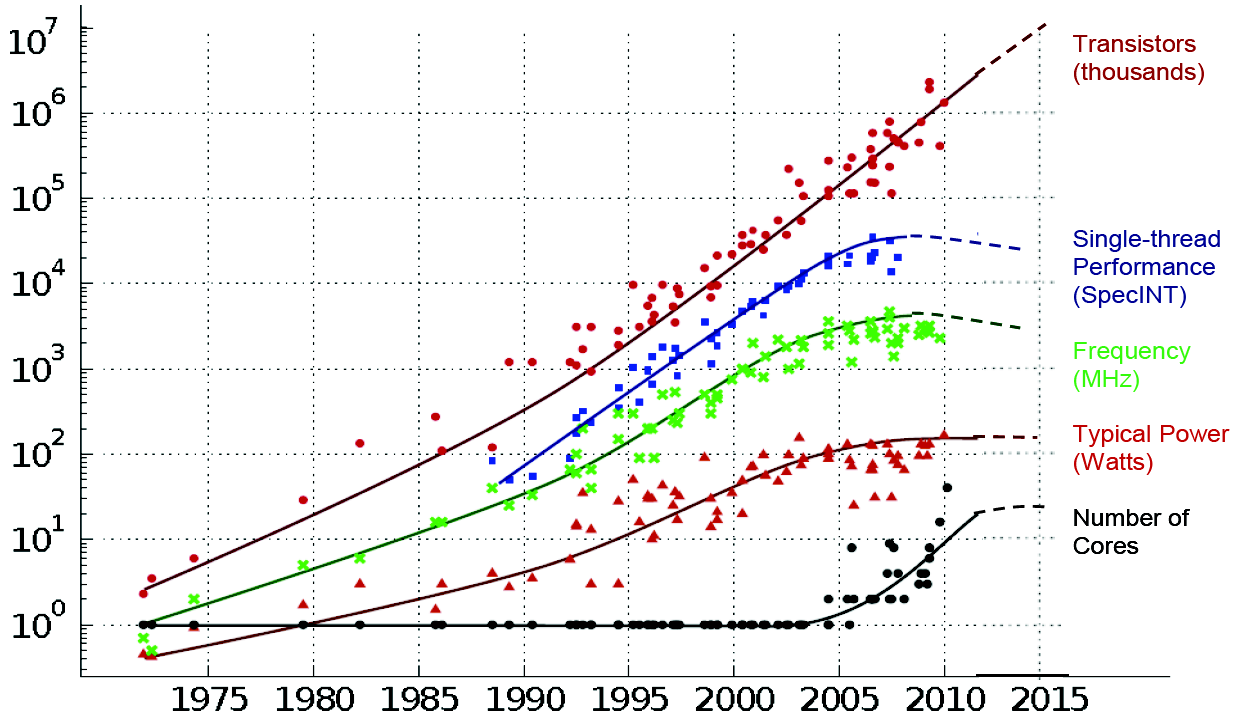
\includegraphics[scale=0.35]{cpu_trands}
\centering
\caption{Evolution des fréquences maximales de processeurs \cite{qaca17}}
\label{fig:FG_2_1}
\end{figure}
%
\subsection{Mémoire}
%
Une caractéristique importante du développement matériel au cours des dernières décennies a été l'écart croissant entre le \textbf{temps de cycle de l'horloge du processeur} et le \textbf{temps d'accès à la mémoire} principale. 
La mémoire principale est construite sur la base de la mémoire \textbf{DRAM (Dynamic Random Access Memory)} qui est trop lente par rapport au cycle d'horloge du CPU.
Les calculs impliquant uniquement le registre du processeur peuvent être effectués rapidement, mais lors d'un accès à la mémoire principale, le processeur se bloque pendant de nombreux cycles en attendant les données de la mémoire avant de pouvoir reprendre l'exécution et cela limite fortement ses performances. Durant cette opération, beaucoup de cycles sont perdus à attendre que des données en mémoire soient mises dans les registres.
Cet écart (de la vitesse entre le processeur et la mémoire) est devenu très grand ce qui rend inutile de continuer cette course qui n'est pas suivie par la mémoire.
En effet, la différence entre la fréquence du processeur et celle de la mémoire est telle que tout accès mémoire devient extrêmement coûteux (memory wall \cite{memw04}).
La figure \ref{fig:FG_2_2} donne l'écart de la vitesse entre le processeur et la mémoire.

\begin{figure}[h]
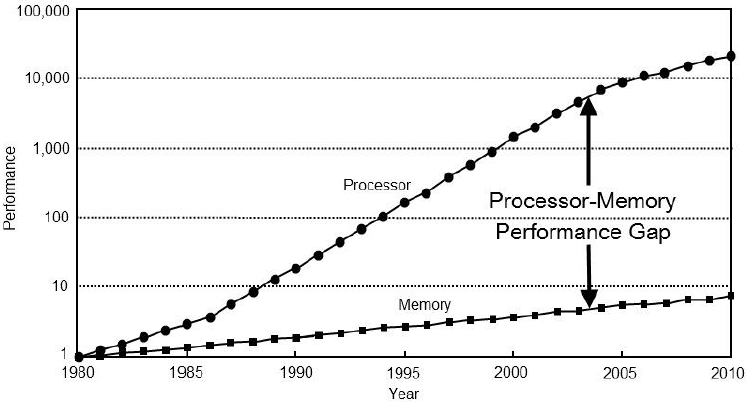
\includegraphics[scale=0.5]{ram_gap}
\centering
\caption{Ecart de la vitesse entre le processeur et la mémoire \cite{memw04}}
\label{fig:FG_2_2}
\end{figure}
%
\subsection{Pipeline ILP( Instruction Level Parallelism)}
%
Le \textbf{parallélisme matériel} a atteint sa limite de 40 étages au delà il y a peu de parallélisme avec un coût important (Extraction du parallélisme au niveau des instructions à partir d’un flot séquentiel bas niveau). 

"L'industrie a été stupéfaite lorsque Intel a annulé non pas un, mais deux modèles de processeurs de premier plan en mai 2004. Intel Tejas (le mono remplaçant de Pentium 4) a dissipé 150 watts à 2,8 GHz avec un pipeline de 40 étages et un socket 1000 pins. Lorsque les microprocesseurs sont trop chauds, ils cessent de fonctionner et parfois explosent." Suite à cet évènement, l'expression "Intel's Tejas hits the walls - hard" a exprimé la situation de l'industrie des microprocesseurs, en marquant la fin de la période des monoprocesseurs .
Ainsi, Intel a rapidement changé de direction, et a annoncé le premier double cœur processeur en lançant la révolution des multicœurs. \cite{russ11}
%======================================================================================================
\section{Processeurs Multicœurs (Multicore)}
%
Le \textbf{processeur multicœurs} est un processeur intégrant plusieurs unités de calcul en les dupliquant sur la même puce. 
On appelle chaque unité un \textbf{cœur (core)} qui est capable de faire un traitement, d'accéder à la mémoire, d'exécuter des entrées/sorties, qui est superscalaire, out-of-order et dispose d’un certain nombre d’unités de calcul vectoriel (Single Instruction Multiple Data ou SIMD). 
L'ensemble des cœurs fonctionne en parallèle en réalisant les tâches affectées (calcule, communication RAM - I/O).

\begin{figure}[h]
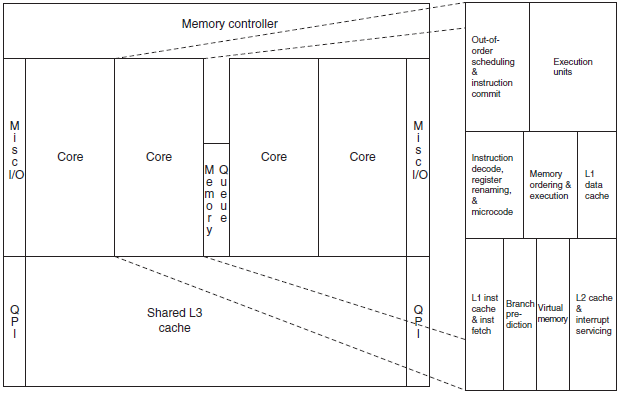
\includegraphics[scale=0.5]{mc_i7_die}
\centering
\caption{Architecture du processeur d'Intel Multicore i7 \cite{qaca17}}
\label{fig:FG_2_3}
\end{figure}

La figure \ref{fig:FG_2_3} montre un exemple d'un processeur multicœurs le processeur \textbf{Intel Core i7}, il dispose de quatre cœurs regroupés par 2. 
%
Chaque cœur a son +propre cache de niveau 1 et 2 (L1, L2) et
Ils ont un cache de niveau 3 (L3) partagé.
D’un point de vue de calcul parallèle, les différences majeures entre les processeurs multicœurs disponibles sont :
%
\subsection{Contrôleur de mémoire intégré}
%
Les fournisseurs des processeurs ont intégré un \textbf{contrôleur de mémoire} et un \textbf{bus} dans la CPU MC pour connecter la mémoire du système à pleine vitesse à ces cœurs. 
Ce connecteur (le bus qui relie les cœurs à l’IMC) est généralement partagé entre tous les cœurs du processeur. %[Coo09, AMD13]
%
\subsection{Hiérarchie de la mémoire \cite{raub13}} 
%
Vu que le système de mémoire est très lent par rapport au processeur et pour utiliser efficacement les cycles de ce dernier et réduire la pénalité de l'accès mémoire (Une puce DRAM a un temps d'accès mémoire entre 20 et 70 ns 
et un processeur à 3 GHz de fréquence, a un temps de cycle de 0.33 ns, un accès mémoire est équivalent à 60–200 cycles processeurs).
Une \textbf{hiérarchie de mémoire} est généralement utilisée, composée de plusieurs niveaux de mémoires de tailles et de vitesses d'accès différentes. La figure \ref{fig:FG_2_4} schématise cette hiérarchie avec ses différents composants et \ref{table:TBhm001} donne les valeurs associées aux métriques quantitatives mesurant ses caractéristiques, seule la mémoire principale au sommet de la hiérarchie est construite à partir de \textbf{DRAM (Dynamic Random Access Memory)}, les autres niveaux utilisent \textbf{SRAM (Static Random Access Memory)}.
L'objectif dans la hiérarchie mémoire est d'avoir un temps d'accès mémoire moyen faible en favorisant l' accès aux données à partir d'une mémoire rapide, et qui contient seulement une partie des données de la mémoire principale lente. 
Sa conception peut avoir une grande influence sur le temps d'exécution des programmes parallèles.

\begin{figure}[h]
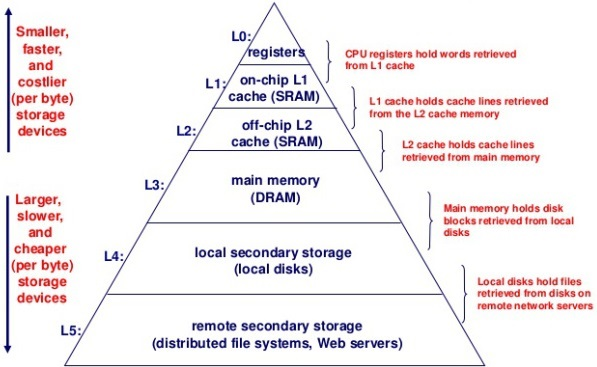
\includegraphics[scale=0.5]{memory_hierarchy01}
\centering
\caption{Hiérarchie de la mémoire}
\label{fig:FG_2_4}
\end{figure} 

\begin{table}[h!]
\centering
\begin{tabular}{| c | c | c | c | c | c | c |} 
\hline
Level                & Register    & Cache L1  & Cache L2  & Cache L3  & Memory  & Disk  \\ [0.5ex] \hline
Technology 		& Gate & SRAM & SRAM & SRAM & DRAM & Flash/Magnetic \\ [1ex]  \hline
Data 				& Word & Line (Bloc) & Line & Line & Page & File \\ [1ex]  \hline
Capacity 		& 1Kbit & 64KB & 256KB & 2-4MB & 1-16GB & 1-16TB \\ [1ex]  \hline
Latency 		& 30ps & 1ns & 3-10ns & 10-20ns & 50-100ns & 5-10ms \\ [1ex]  \hline
\end{tabular}
\caption{Caractéristiques de la hiérarchie mémoire : \cite{qaca17}} %
\label{table:TBhm001}
\end{table}
%
\subsection{Caches}
%
Tous les processeurs modernes sont équipés d'une mémoire de petite capacité (allant de quelques Ko à quelques Mo) mais très rapide (0.5-2.5 ns comparé au DRAM 50-70ns %[BK-MC-84]
) appelée \textbf{cache} SRAM qui stockent des données (une partie des données de la mémoire) sur lesquelles le processeur travaille temporairement et qui masquent la \textbf{latence d'accès} à la mémoire principale lente.
L'emplacement physique de la mémoire cache est très proche des cœurs afin de réduire les coûts de communication.

Dans une configuration typique, un CPU comprend plusieurs caches, formant une \textbf{hiérarchie de cache} %@[SZ08, OHSJ10].
Les caches peuvent être une autre ressource partagée sur les processeurs.

Le \textbf{cache de premier L1} est local pour chaque cœur de petite taille, comprise entre 8 et 128 kilo-octets, mais assez rapide. 

Le \textbf{cache du deuxième niveau L2} peut être local pour chaque cœur ou partagé entre les cœurs moins rapide que L1 et mais de taille supérieure, L1 et L2 sont partagés entre les \textbf{threads matériels}.

Le \textbf{cache de troisième niveau L3}, cependant, est partagé entre tous les cœurs du processeur de grande taille mais lent %[SZ08].

Les caches stockent les blocs de données des niveaux supérieur sous la forme de \textbf{lignes de cache = bloc} : un bloc contigu d'octets.  La taille est fixe, dépend de l'architecture, typiquement elles sont de 32 octets sur certains processeurs de l'architecture ARM [Lim07], ou 64 octets sur les processeurs x86 de l'architecture Netburst d'Intel %[Coo13b].

Grace à un \textbf{contrôleur de cache} séparé, le contrôle du cache est découplé du processeur et exécuté par ce dernier.
Pendant l'exécution du programme, 
le processeur spécifie les adresses mémoire (indépendamment de l'organisation du \textbf{système de mémoire}, sans connaître l'architecture) à lire ou à écrire comme données par les opérations de chargement/stockage. %1
il les transmet à ce système et attend que les valeurs correspondantes soient renvoyées ou écrites. %2
Après avoir reçu une requête d'accès mémoire du processeur, 
le contrôleur de cache vérifie si l'adresse mémoire spécifiée correspond à une ligne de cache qui est actuellement stockée dans le cache. %3
Si c'est le cas, une \textbf{mise en cache cache-hit} se produit et la donnée demandée est transmise au processeur à partir du cache. %4.1
Sinon un \textbf{cache manqué cache-miss} se produit et 
la ligne de cache est d'abord copiée de la mémoire dans le cache (un bloc de mémoire entier est amené dans le cache, dit un \textbf{remplacement cache})
avant que la donnée demandée ne soit délivrée au processeur. %4.2
%
Le temps de retard correspondant est appelé \textbf{pénalité du cache-miss}. 
%
Étant donné que le temps d'accès à la mémoire est significativement plus grand que le temps d'accès au cache, un cache-miss entraîne un retard de remise d'opérande au processeur.
Par conséquent, il est souhaitable de réduire autant que possible le nombre des cache-miss.
%
Le temps d'accès d'un cache dépend de sa taille, la taille du bloc-cache et sa méthode d'adressage, 
%
Toutefois, l'utilisation d'un cache plus grand entraîne un plus petit nombre de remplacements par rapport un cache plus petit, car davantage de blocs de cache peuvent être conservés dans le cache. 
%
L'utilisation de blocs plus grands réduit le nombre de blocs qui s'intègrent dans le cache lors de l'utilisation de la même taille de cache. Par conséquent, les blocs ont tendance à être remplacés plus tôt par rapport aux blocs plus petits. 

Étant donné que le cache est nettement plus petit que la mémoire principale, tous les blocs de mémoire ne peuvent pas être stockés dans le cache en même temps. 
Par conséquent, un \textbf{algorithme d'association} doit être utilisé pour définir la relation entre les blocs cache/mémoire ($BC$/$BM$) et détermine comment un bloc stocké est localisé et extrait du cache.
Pour l'association, l'accès associatif clé(tag)/valeur(contenu du $BM$) sera utilisé pour déterminer pour un bloc-mémoire les positions des blocs-cache ou il peut être stocké/sa position dans le cache pour une mise à jour ou une lecture, s'il est déjà chargé dans le cache. \cite{Hunold07}
%
\subsubsection{Méthodes de Remplacement des blocs}
%
Lorsqu'un cache-miss se produit, un nouveau bloc de mémoire doit être chargé dans le cache. Dans ce cas, il faut choisir la position dans le cache pour stocker le nouveau bloc mémoire alors il faut décharger le bloc occupant cette position.
Le bloc à remplacer est sélectionné en utilisant une méthode de remplacement.

- \textbf {Le moins récemment utilisé (Least recently used LRU)} qui remplace le bloc d'un ensemble qui n'a pas été utilisé depuis un certain temps.
le matériel doit garder une trace pour chaque bloc d'un ensemble lorsque ce dernier a été utilisé récemment et son temps d'accès correspondant doit être mise à jour à chaque utilisation.

- \textbf{Le moins fréquemment utilisé (Least frequently used LFU)} qui remplace le bloc d'un ensemble qui est le moins référencé (peu d'accès à ce bloc).
pour chaque bloc un compteur doit être maintenu par LFU qui doit être mis à jour pour chaque accès mémoire.
%
\subsubsection{Politique de modification (Write Policy)}
%
Lorsque le processeur émet un accès en écriture à un bloc de mémoire actuellement stocké dans le cache, le bloc référencé est définitivement mis à jour dans le cache, car l'accès en lecture suivant doit renvoyer la valeur la plus récente (most recent value MRV).
Quand le bloc mémoire correspondant dans la mémoire principale est-il mis à jour? La stratégie qui prend cette décision est appelé \textbf{politique d'écriture ou de modification}. Les politiques les plus utilisées sont :

- \textbf{Modification immédiate (Write-Through)}
la mise à jour de la mémoire est faite immédiatement âpres la modification du BC ce qui permet de garder la mémoire et le cache dans un état consistant. 
son inconvenant est que chaque modification cache déclenche un accès mémoire.

- \textbf {Modification retardée (Write-back)}
Une opération d'écriture d'un bloc de mémoire actuellement réside dans le cache est effectuée uniquement dans le cache; l'entrée de mémoire correspondante n'est pas mise à jour immédiatement. Ainsi, le cache peut contenir des valeurs plus récentes que la mémoire principale.
%
\subsection{Cohérence de Cache}
%
Pour les systèmes multiprocesseurs-multicœurs où chaque processeur/cœur utilise un cache local séparé, nous sommes confrontés au problème de conserver une vue cohérente des données partagées entre tous les processeurs/cœurs. 
Les données partagées stockées à des niveaux différents dans la hiérarchie de la mémoire peuvent conduire à un \textbf{problème de cohérence de cache} qui peut être défini lorsque les différents cœurs du processeur copient les mêmes informations de la mémoire/cache partagé, et que diverses copies des données seront stockées dans le cache de chaque cœur, surtout si la politique write-back est utilisée.
Par conséquent, chaque copie de données peut avoir une valeur distincte des copies des 'autres cœurs après qu'elle est traitée séparément, elle est alors appelée \textbf{copie incohérente (invalide)}. \cite{raub13}
Alors comment garder les différentes copies d'une donnée mémoire consistantes et système doit assurer l'accès à la \textbf{valeur mise a jour récemment (most recent value MRV)}?

La \textbf{cohérence des informations} entre mémoire-cache et cache-cache est un élément fondamental car elle garantit qu'un processeur/cœur a accès à la dernière valeur qui a été écrite.
Pour être cohérent, le système de mémoire doit satisfaire certaines propriétés en assurant que chaque processeur a une vue cohérente et que lui même a une \textbf{vue globale cohérente}.
Pour réaliser cet objectif, un protocole de cohérence de cache basé sur le matériel est utilisé. 
De nombreux protocoles peuvent être identifiés, y compris les protocoles de surveillance et les protocoles basés sur les répertoires.
%
\subsubsection{Protocole de surveillance}
%
Ce protocole repose sur la propriété que tous les accès mémoire sont effectués via un \textbf{support partagé de diffusion} (un bus)
de sorte que chaque contrôleur de cache puisse observer tous les accès en écriture pour effectuer des mises à jour ou des invalidations.
Ainsi, toutes les entrées peuvent être observées par les contrôleurs de cache de chaque processeur. 
Lorsque le contrôleur de cache observe une écriture dans un emplacement de mémoire actuellement détenu dans le cache local, il déclenche un mécanisme pour préserver la cohérence.
il a deux techniques :

\textbf{protocoles basés sur des mises à jour} :
Les contrôleurs de cache effectuent directement une mise à jour du cache en copiant la nouvelle valeur à partir du bus. 
Ainsi, les caches locaux contiennent toujours les valeurs écrites les plus récentes des emplacements de mémoire. 

\textbf{protocoles basés sur l'invalidation} :
Dans ce cas, le bloc de cache correspondant à un bloc de mémoire 
est invalidé de sorte que l'accès en lecture suivant doit d'abord effectuer une mise à jour à partir de la mémoire principale. \cite{Tan02}
%
\subsubsection{Protocole basé sur l'annuaire}
%
Ce protocole est une alternative au protocole de surveillance, au lieu d'utiliser un support de diffusion, il utilise un \textbf{répertoire central} pour stocker l'état des blocs de mémoire qui peuvent être conservés dans le cache. 
un contrôleur de cache peut obtenir l'état d'un bloc de mémoire par une recherche dans le répertoire. 
Ce répertoire peut être partagé ou réparti entre différents processeurs pour éviter les conflits d'accès. \cite{Culler99}

Un répertoire central est maintenu pour sauvegarder l'état de chaque bloc mémoire qui est déjà copié dans un cache. Ce répertoire peut être partagé. Le contrôleur de cache détermine l'état d'un  bloc en accédant et en consultant ce répertoire.

%=====================================================================================================================================
\section{Systèmes SMP/UMA (uniform memory access)}
%
Ils sont des multiprocesseurs à mémoire partagée via un bus commun, comportent un petit nombre de processeurs, généralement huit ou moins souvent appelés \textbf{Multiproce-sseurs symétriques (à mémoire partagée) (SMP)}.
Vue leurs conception architecturale, Les SMP et les MC ont en commun une contrainte qui limite leurs performances, la mémoire centrale partagée et l'accès à un espace d'adressage commun pour toutes les unités de traitement (soit processeurs ou cœurs). 
Toutes ces unités ont un temps d'accès égal à cette mémoire (un temps d'accès à la mémoire uniforme pour tout le monde UMA), d'où le terme \textbf{symétrique} ou l'\textbf{uniformité}. 

Un algorithme séquentiel $A_s$ parallélisé ($A_p$) pour être exécuté sur une architecture UMA peut ne pas atteindre les performances espérées préalablement (gain en rapidité et la réduction significative du temps total d'exécution $C_{max}$) pour plusieurs raisons qui peuvent être liées à 
 sa nature, 
à la méthode de la décomposition parallèle ou 
aux contraintes des architectures cibles. 
Avant d'exposer ces facteurs, nous présentons les métriques qui permettent de mesurer le gain de l'exécution parallèle sur une architecture cible par rapport son exécution séquentielle.
%
\subsection{Mesure de l'accélération (speedup $\gamma$)} 
%
\begin{définition}[Accélération d'un programme parallèle.]\textit{
%
En donnant un algorithme séquentiel $A_p$ dont le temps d'exécution séquentielle sur un processeur est $T_1$ , 
Soit $A_p$ sa version parallèle et $T_p$ son temps total d'exécution sur l'architecture parallèle cible $\mathbb{H}$.
L’\textbf{accélération} de $A_p$ représente le gain en rapidité d’exécution obtenu par son exécution sur $\mathbb{H}$ qui est égale au rapport entre le temps d’exécution du programme séquentiel et le temps d’exécution parallèle en fonction du nombre des ressources parallèles dans la plateforme (processeurs).
$$\gamma(n) = \frac{T_1}{T_p}$$
}\end{définition}
%
Si ce rapport est constant alors l’accélération est linéaire dans ce cas elle représente un parallélisme optimal (idéal). 
Mais s’il est variable sa courbe représente une accélération sub-linéaire (au dessous de la ligne $y=x$) alors ce ralentissement dû au overhead du parallélisme causé par la communication et la synchronisation.

La décomposition d’un programme parallèle influence sur ce facteur. Et puisque cette décomposition est fonction degré intrinsèque de parallélisation de l'algorithme séquen-tiel (
L’existence d'une partie purement séquentielle $T_s$ et d'une partie parallélisable $T_p$ tel que $T_1 = T_s + T_p$ avec un taux de parallélisation $\alpha_p = T_p/T_1$) . 
La \textbf{loi d'Amdahl} raffine l'expression de $gamma$ en fonction de cette décomposition et le nombre des processeurs $p$ de la plateforme parallèle, par la formule suivante \cite{raub13}:

$$ \gamma = \frac{T_1}{T_s + T_p/p} = \frac{1}{(1-\alpha_p) + \alpha_p/p}$$

On remarque que si $\lim_{p \to \infty} \gamma = 1/(1-\alpha_p)$ alors cette accélération est limitée par la partie non parallélisable de $A$. Et si $\lim_{\alpha_p \to 1} \gamma = p$ ça donne une accélération linéaire (un parallélisme optimal).

Cette mesure $\gamma$ exprime une valeur théorique qui ne prend pas en compte l'influence des opérations de la communication et la synchronisation entre les parties parallèles entre elles-mêmes ou avec la hiérarchie mémoire d'une part et l'impact de l'architecture de la plateforme parallèle (ses caractéristiques, sa topologie, ) avec son support d'exécution (runtime, ordonnanceur, mapper, ...) d'autre part. Ces deux facteurs ajoutent un overhead non négligeable aux processus de la parallélisation. 
Bien que les caches, la préextraction(pre-fetching) et les canaux de communication améliorent considérablement les performances si elles sont exploitées efficacement, pas tous les accès à la mémoire principale peuvent être éliminés et ou les communications entre les parties parallèles l'amélioration de la latence d'accès DRAM et la minimisation de l'impact de la communication/synchronisation reste une préoccupation majeure pour les performances.

Dans le contexte des architectures SMP/multicœur,
un système parallèle de $p$ unités de traitement (processeur/cœur), chaque unité supplémentaire augmente potentielle-ment le nombre total de demandes à la mémoire principale par unité de temps $t$ et le nombre des opérations communication/synchronisation $Q_M(p,t)$ et augmente ainsi la pression sur le contrôleur de mémoire et sur bus partagé en réduisant la bande passante et augmentant la latence d'accès à la DRAM $L_M(p,t)$. 

$$Q_M(p,t) \leq Q_M(p+1,t) \Rightarrow L_M(p,t) > L_M(p+1, t)$$

Pour $p_0$ suffisamment grand $L_M(p_0, t) >>$ devient important. Une fois la bande passante du contrôleur saturée, la latence des accès à la DRAM augmente et les accès mémoire deviennent rapidement un goulot d'étranglement pour les performances qui augmentent le temps des communications et par conséquent le temps total d'exécution $C_{max}$ .\\
%
\subsection{Passage à l’échelle (scalability $\zeta$)}
%
\begin{définition}[Accélération d'un programme parallèle.]\textit{
%
La scalabilité ($\zeta$) d’un programme parallèle désigne l’augmentation des performances ($\Phi$) obtenues lorsque l’on ajoute des processeurs $p$ : 
$$\zeta_p =\Delta(p) = \Phi(q+p)/\Phi(q)$$
%
}\end{définition}

La scalabilité mesure l'évolutivité qui est le degré auquel le débit de charge de travail $W$ bénéficie de la disponibilité de processeurs supplémentaires ou la faculté d'un système de maintenir un niveau de performance stable $\Phi_c$.
Il est généralement exprimé comme le quotient du débit de la charge de travail $W_p$ sur un multiprocesseur divisé par le débit sur un monoprocesseur comparable $W_1$ : $\zeta_p = W_p/W_1$.
%ref http://www.perfdynamics.com/Manifesto/USLscalability.html.
Dans leurs travaux Gunther .al propose un modèle pour quantifier la scalabilité de façon générale. Le modèle proposé USL (Universal scalabilité law) \cite{Gun17} combine les effets suivants en définissant un modèle de scalabilité unifiée dont le coefficient de scalabilité C(N) : 
%
$$ C(N) = \frac{N}{1 + \alpha (N - 1) + \beta N (N - 1)}$$
%
Les termes du dénominateur expriment les aspects suivants (les niveaux \textbf{3Cs}) :\\
- \textbf{Concurrence}: (parallelism ideal): basically, linear scaling (Computation) .\\
- \textbf{Contention}: due aux files d'attente des ressources partagées(Communication $\alpha$)\\  %overhead 
- \textbf{Cohérence}: due au retard de la mise à jour des données dans la hiérarchie mémoire (rendre les données consistantes et cohérentes) ($\beta$).

Dans le contexte des machines parallèles récentes, nous pouvons inclure les facteurs ignorés dans la loi d'Amdahl en définissant un speedup $\gamma$ étendu exprimé en fonction du parallélisme intrinsèque de la l'algorithme séquentiel (la partie parallélisable) et son overhead de la communication/synchronisation $\beta_c$ généré par son exécution parallèle sur la plateforme cible (la configuration de la plateforme c.-à-d. sa topologie, sa hiérarchie mémoire, son réseau d’interconnexion,). 
%
$$\gamma(n) = \frac{1}{(1-\alpha_p) + \alpha_p/p + \beta_c} = h( \text{algorithme\_parallèle , plateforme\_configuration})$$
%
\begin{figure}[h]
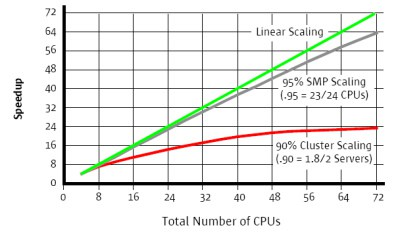
\includegraphics[scale=0.5]{scalability001}
\centering
\caption{Scalabilité linéaire, SMP et Cluster  \cite{qaca17}}
\label{fig:FG_2_5}
\end{figure}
%
La figure \ref{fig:FG_2_5} présente la scalabilité de certaines plateformes informatiques. Elle donne la mesure de l'accélération résultant du processus de la parallélisation d'une application sur une plateforme parallèle constituée de plusieurs processeurs.

L'expérimentation a démontré que les charges de travail réelles ne s'adaptent pas parfaitement à un système SMP à partir de certain seuil. 
Dans ce contexte, les principaux facteurs qui empêchent une scalabilité parfaite sont les suivants :\\
%
- \textit{La contention bus/mémoire augmente (toute la mémoire est partagée par tous les proces-seurs)}\\
- \textit{L'augmentation du coût/nombre des échecs caches (ratés)}\\
- \textit{Le cache invalidation des caches distants (lire un cache distant pour maintenir la cohérence du cache)}\\
- \textit{Augmentation du coût / nombre des instructions de synchronisation / verrouillage - déverrouillage / attente de verrous utilisés par le système d'exploitation et applications}.

Tous ces facteurs contribuent négativement à achever un niveau de scalabilité acceptable sur SMP pour des charges de travail moyennes ou importantes. 
C'est difficile dans ces conditions (SMP-mémoire partagée avec un bus d'accès unique) de préserver un niveau stable des performances en ajoutant d'autre processeurs à partir de certain seuil $p_0$ par contre toute augmentation va avoir un effet négatif sur la performance 
(Problème de scalabilité : $ \forall p > p_0, \zeta_p \leq \zeta_{p-1}$)
%======================================================================================
\section{Systèmes NUMA Non Uniform memory Access}
%
NUMA est une solution pour surmonter les problèmes de la scalabilité des architec-tures SMP \cite{lak-pan}, basée sur le principe d'une mémoire distribuée et partagée ou les processeurs accèdent à tout l'espace mémoire disponibles.
Chaque processeur est directem-ent connecté à une partie de la mémoire physique (un banc mémoire). Un exemple d'une carte mère NUMA  à quatre nœuds constitués d'un microprocesseur et d'un banc mémoire est donné dans la figure \ref{fig:FG_2_6}. La deuxième figure \ref{fig:FG_2_7} montre l'architecture typique d'une plateforme NUMA deux variantes présentées à deux nœuds et à plusieurs nœuds respectivement.
%
\begin{figure}[h]
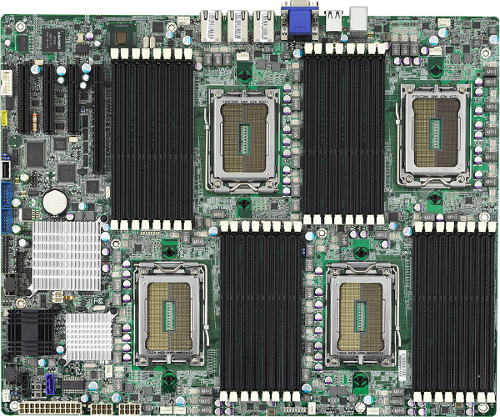
\includegraphics[scale=0.5]{mother_board_numa}
\centering
\caption{Carte mère NUMA}  % sr0c : \cite{ctan}}
\label{fig:FG_2_6}
\end{figure}
%
\begin{figure}[h]
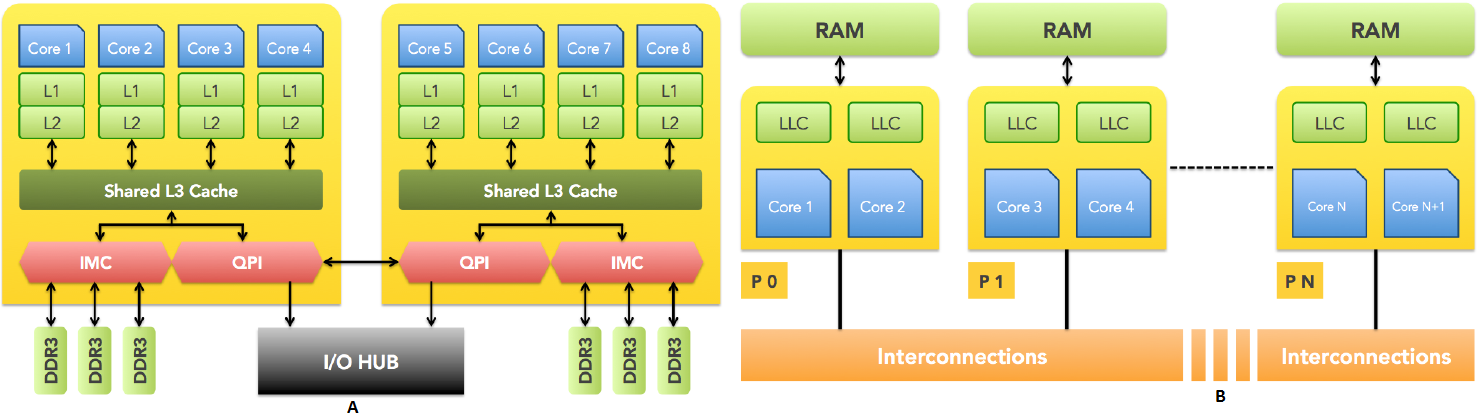
\includegraphics[scale=0.4]{numa001}
\centering
\caption{Architecture NUMA (a) Plusieurs nœuds (b) à deux nœuds }  % sr0c : /cite{ctan}}
\label{fig:FG_2_7}
\end{figure}
%
\subsection{Architecture NUMA}
Son architecture est constituée de composants suivants : 
%
\subsubsection{Nœud (Node, Socket)}
Un nœud peut être un processeur multicœurs ou un SMP constitué de plusieurs processeurs multicœurs qui se caractérise par l'uniformité de l'accès à la mémoire de tous ces composants (UMA).
%
\subsubsection{Réseaux d'interconnexion (Interconnexion network ICN)}
Un réseau de liens de communication de haut débit et de faible latence, les échanges sont établis via une connexion sur ce réseau (déterminer le chemin entre deux communicants, un routage). %deux types existe de cet ICN : 
Ce réseau est caractérisé par sa topologie déterminée par la façon de connecter les nœuds des plateformes. Deux classes de topologies existent :

A- \textbf{Topologie point-a-point (entièrement maillé)} : permet de connecter tous les nœuds en direct (un seul saut) 
Ce type de topologie dégrade les performances lors du passage à l'échelle pour un réseau moyen ou important de processeurs connectés vu que le nombre des liens requis est quadratique $O(n^2)$.

B- \textbf{Topologie spécifique avec un mécanisme de routage} : Elle peut être un arbre ou anneau ou autre avec des caractéristiques géométriques spécifiques qui permettent de déterminer la longueur du chemin pour relier deux processeurs communicants. 
Les processeurs distants sont accessibles par plus d'un saut en plusieurs étapes intermédiaires à travers d’autres processeurs. 
Le mécanisme de routage permet de déterminer le chemin menant au processeur cible à partir de la source ensuite acheminer les requêtes distantes aux processeurs cibles pour lire ou écrire une information dans sa mémoire locale à la demande du processeur source. 

Parmi les ICNs implémentés sur les plateformes NUMAs modernes, nous pouvons citer \cite{dan-mul} : \\
-a- \textbf{QPI} : QuickPath Interconnect (QPI) Intel \cite{IntelQPI09}\\
-b- \textbf{HT} : HyperTransport AMD \cite{amdHT}\\
-c- \textbf{FP}: Fireplane interconnect Sun Microsystems \cite{Char02}.
%
\subsubsection{Mémoire distribuée-partagée}
%
Le système de mémoire est hybride, une mémoire distribuée-partagée, physiquement distribuée sur les nœuds et partagée entre es cœurs de même nœud. L'espace d'adressage est global et partagé, n'importe quelle unité de calcul peut accéder à n'importe quelle adresse mémoire. Dans ce contexte, nous distinguons deux types de mémoire :\\
%
a - \textbf{Mémoire locale} : des bancs de mémoire associée à chaque processeur et directement connectés caractérisés par un accès local en écriture en lecture aux données situées dans sa mémoire locale qui est assez rapid. La figure \ref{fig:FG_2_num010} schématise les accès mémoire sur une plateforme NUMA et coût correspond en fonction des cycles processeur. Pour les accès locaux, Elle donne 38 cycles pour le cache local et 190 cycles pour la mémoire locale.\\
%
b - \textbf{Mémoire distante} : qui, du point de vue d'un CPU, est connectée à un CPU différent, caractérisée par un accès distant en écriture ou en lecture aux données situées dans une mémoire distante qui assez lent. % comme la mémoire globale est distribuée (locale à un processeur différent)
Sur la figure \ref{fig:FG_2_num010}, Pour les accès distants, Les valeurs données sont 186 cycles pour le cache distant et 310 cycles pour la mémoire distante.
%
\begin{figure}
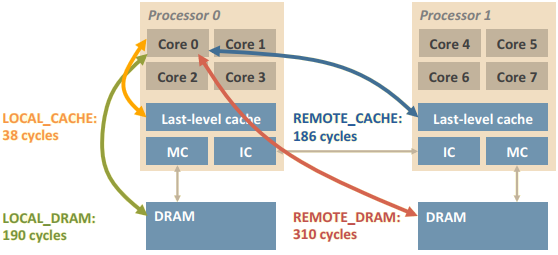
\includegraphics[scale=0.75]{num010}
\centering
\caption{Accès mémoire locaux et distants sur NUMA}
\label{fig:FG_2_num010}
\end{figure}
%
La figure \ref{fig:FG_2_num0092} présente un exemple d'un code OPENMP qui s'exécute sur NUMA en parallélisant une boucle dont les données sont deux vecteurs $A$ et $B$. Chaque itération va lire une valeur de $A$ ($A[i]$) et modifie une valeur de $B$ ($A[i]$). La parallélisation de la boucle crée un ensemble de tâches (thread) pour exécuter un nombre spécifié d'itérations. Donc chaque tâche nécessite d'accéder à la plage affectée des valeurs de $A$ et $B$ pour faire son calcul. Si les vecteurs $A$ et $B$ sont distribués sur les mémoires de la plateforme (le cas présenté par la figure), et la plage des éléments de $A$ et $B$ utilisés par la tâche $T$ est stockée dans la mémoire du nœud $N$ sur lequel $T$ s'exécute, alors les $T$ n'aura que des accès locaux. Par contre si une partie de ces éléments sont stockés sur une autre mémoire alors Certain nombre d'accès mémoire de $T$ seront distant et cela va prolonger l'exécution de $T$. Les tables \ref{table:TB_2_14520} et \ref{table:TB_2_1453} donnent le coût en cycle processeur, temps d'accès (local, voisin et voisin distant) et bande passante/latence respectivement des accès mémoire en fonction de leurs nature et emplacement. Ca donne une idée de l'impact du type d'accès sur le déroulement de l'exécution des tâches (en réduisant/augmentant le nombre de cycles processeur ou temps d'accès ou latence/BP).
%
\begin{table}[h!]
\centering
\begin{tabular}{| c | c | c | c |} 
\hline
			& CACHE		& MEMORY 	& BANDWIDTH \\ [0.5ex] \hline
LOCAL  	& 38 cycles   	& 190 cycles 	& 10.1 GB/s      \\ [0.5ex] \hline
REMOTE 	& 186 cycles 	& 310 cycles 	& 6.3 GB/s       \\ [1ex]  \hline
\end{tabular}
\caption{Coût des accès mémoire en cycles processeur et la bande passante} %
\label{table:TB_2_14520}
\end{table}
%
\begin{figure}
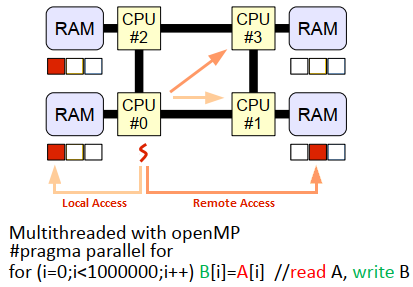
\includegraphics[scale=0.75]{num0092}
\centering
\caption{Code OPENMP parallélisant une boucle sur NUMA}
\label{fig:FG_2_num0092}
\end{figure}
%
\begin{table}[h!]
\centering
\begin{tabular}{| c | c | c | c |} 
\hline
			& LOCAL NODE		& NEIGHBOR NODE & OPPOSITE NODE\\ [0.5ex] \hline
READ  	& 83 ns   	& 98 ns  	& 117 ns\\ [0.5ex] \hline
WRITE 	& 142 ns 	& 177 ns  & 208 ns\\ [1ex]  \hline
\end{tabular}
\caption{Coût des accès mémoire mesuré en temps d'accès pour l'exemple figure \ref{fig:FG_2_num0092}} %
\label{table:TB_2_1453}
\end{table}
%
\subsection{Caractéristiques NUMA}
%
\subsubsection{Pénalité NUMA (ratio)}
%
Comparé à un accès local, l'accès distant est caractérisé par un débit faible et latence importante. En se basant sur cette réalité dans les plateformes NUMA, nous pouvons définir une métrique qui évalue l'efficacité des politiques des gestions des ressources NUMA en fonction des ces deux types d'accès. Cette métrique est appelée ratio NUMA (distance, NUMA rate, factor).
La pénalité NUMA $\alpha$ est le rapport du nombre d'accès local $A_L$ sur le nombre des accès distant $A_R$ pour le programme $P$ en court d'exécution sur une plateforme NUMA spécifique. 
Cette métrique est pour quantifier l'overhead généré par la communication entre les nœuds de la plateforme lors de cette exécution \cite{dan-mul}
%
$$
\alpha(P) = \frac{A_L}{A_R}
$$
%
\subsubsection{Distance NUMA (sauts NUMA))}
%
Les architectures à base de NUMA introduisent une notion de distance entre les composants du système (ie: nœuds, processeurs, mémoire, bus d'E/S, etc.). 
La métrique utilisée pour déterminer une distance(saut) entre les nœuds NUMA varie avec la latence et la bande passante. 
%
\subsubsection{Cohérence de Cache NUMA (ccNUMA)}
%
La mémoire globale est partagée et chaque processeur peut accéder à n'importe quel élément de données, bien qu'avec des performances réduites si l'élément de données est situé sur une banque de mémoire qui n'est pas directement connectée.
Cependant, la mémoire cache interne non partagée de chaque processeur (ou de chaque nœud pour les processeurs multi-nœuds) n'est pas accessible depuis d'autres processeurs. 
Un processeur ne sait donc pas si l'état d'un élément de données dans la mémoire principale est dans un état actuel ou si un état plus mis à jour existe dans un cache d'un autre processeur.
Ainsi, les plates-formes NUMA utilisent un mécanisme pour appliquer la cohérence du cache à travers la mémoire partagée adapté NUMA.

La plupart des systèmes NUMA sont cependant cohérents avec le cache et sont officiellement appelés plateformes ccNUMA.
Les plates-formes ccNUMA utilisent un maté-riel spécial qui permet la communication entre processeurs et les contrôleurs de cache basé généralement sur la technique du répertoire.
Pour chaque cache-manqué (lecture ou écriture), chaque processeur doit communiquer avec tous les autres processeurs afin de s'assurer que le prochain chargement de la mémoire principale est dans un état actuel et non stocké dans un autre cache.
Cette communication a un surcoût significatif.
Afin de réduire cette surcharge, nous devons éviter l'accès à la même zone de mémoire par plusieurs processeurs.
%De plus, les plateformes NUMA utilisent des protocoles de cohérence de cache spécialisés comme MOESI et MESIF qui tentent de réduire la quantité de communication entre les processeurs.
\subsubsection{Exemple}
%
IBM® Power 750 Express® \cite{IBM13} , est un système NUMA. Il est équipé de quatre cartes processeurs, et chacune contient huit cœurs et huit emplacements mémoire (considé-rées locales). Le système contient 32 cœurs et 256 Go mémoire et quatre nœuds NUMA chacun avec 8 cœurs et 64 Go mémoire locale. 
Avec le mode SMT4 (Simultaneous Multith-reading) activé, les systèmes d'exploitation voit 128 (32*4) processeurs logiques avec 32 sur chaque nœud.
Le listing suivant donne le résultat de l'exécution de la commande \textbf{numactl hardware} \cite{Linux13} sur ce système .
%
\begin{Verbatim}[formatcom=\color{blue}]
numactl hardware
available: 4 nodes (0-3)

node 0 cpus: 012 3 4 5 6 7 8 9 10 11 12 13 14 .... 25 26 27 28 29 30 31
node 0 size: 61184 MB
node 0 free: 59734 MB

node 1 cpus: 32 33 34 35 36 37 38 39 40 41 42 .... 57 58 59 60 61 62 63
node 1 size: 65280 MB
node 1 free: 63848 MB

node 2 cpus: 64 65 66 67 68 69 70 71 72 73 74 .... 89 90 91 92 93 94 95
node 2 size: 65024 MB
node 2 free: 63426 MB

node 3 cpus: 96 97 98 99 100 101 102 103 104 .... 123 124 125 126 127
node 3 size: 65024 MB
node 3 free: 63631 MB

node distances:
node 0 1 2 3
0: 10 20 20 20
1: 20 10 20 20
2: 20 20 10 20
3: 20 20 20 10
\end{Verbatim}
%
%La figure suivante \ref{fig:FG_2_ArchNUMA001} montrent un exemple d'une topologie reélle d'une plateforme NUMA extraite par l'outil HWLOC. Chaque nœud a huit cœurs et une mémoire privée de 16Go et un cache L3 de 5Mo.
%
%\begin{figure}
%\includegraphics[scale=1]{ArchNUMA001}
%\centering
%\caption{Topologie réelle d'une plateforme NUMA extraite par l'outil HWLOC}
%\label{fig:FG_2_ArchNUMA001}
%\end{figure}
%
\section{Localité des données et Politiques de Placement}
%
\subsection{Principe de la localité}
%
Le principe de localité est une propriété de programme en exécution qui établie que : 
les programmes ont tendance à \textbf{réutiliser les données et instructions} qu'ils ont utilisées récemment. 
(Un programme consacre 90\% de son temps d'exécution à seulement 10\% du code). 
Ce principe permet de prédire quelles instructions et données un programme utilisera dans un avenir proche en fonction de ses accès dans un passé récent. 
Il s'applique aux accès aux données et code. Il existe des types communs de localité de référence utilisés dans les architectures informatiques. 
La localité spatiale et temporelle peut être distinguée comme suit:
%
\subsubsection{Localité spatiale}
%
Les accès mémoire d'un programme ont une grande localisation spatiale, si le programme accède souvent à des emplacements de mémoire avec des adresses voisines à des moments successifs pendant l'exécution du programme. 
Ainsi, pour les programmes avec une grande localisation spatiale, il arrive souvent qu'après un accès à un emplacement de mémoire, un ou plusieurs emplacements de mémoire de la même ligne de cache soient également accédés peu de temps après. 
Dans de telles situations, après le chargement d'un bloc de cache, plusieurs des emplacements de mémoire suivants peuvent être chargés à partir de ce bloc de cache, évitant ainsi des erreurs de cache coûteuses. 
L'utilisation de blocs de cache comprenant plusieurs mots de mémoire repose sur l'hypothèse que la plupart des programmes présentent une localité spatiale. \cite{Ken02}
%
\subsubsection{Localité temporelle}
%
Les accès mémoire d'un programme ont une forte localisation temporelle, s'il arrive souvent que le même emplacement mémoire soit accédé plusieurs fois à des moments successifs au cours de l'exécution du programme. 
Ainsi, pour les programmes avec une haute localisation temporelle, il arrive souvent qu'après avoir chargé un bloc de cache dans le cache, les mots de mémoire du bloc de cache soient accédés plusieurs fois avant que le bloc de cache soit à nouveau remplacé. \cite{Ken02}
%En ce qui concerne la localité temporelle, la situation est la suivante: après le chargement d'un bloc de cache en raison d'un accès à la mémoire, l'emplacement de mémoire correspondant n'est accédé qu'une seule fois avant que le bloc de cache soit à nouveau remplacé. \cite{Ken02}
\subsection{Politiques de Placement}
%
L'\textbf{affinité des processus et des données} est cruciale pour gérer les problèmes causés par l'\textbf{effet NUMA}, 
ce principe consiste à préserver la proximité de threads et leurs données en en allouant aux données l'espace mémoire associées au nœud sur lequel le thread s'exécute. 
Si un thread accède à la mémoire distante, le thread peut changer son affinité CPU à exécuter localement à la mémoire ou la mémoire peut migrer vers le thread d'accès.
Ces problèmes NUMA peuvent être réduits en maintenant ou en améliorant la proximité de threads et leurs données les plus fréquemment utilisées. 
Afin d'optimiser explicitement une application pour une architecture NUMA multicœurs. 
Ce but est réalisé en sélectionnant une politique de placement appropriée qui place les threads et données en respectant leurs affinités. 
Cette politique essaye de trouver un compromis entre affectation des processeurs aux threads et l'allocation de la mémoire aux données accédées par ces threads. 
%
La figure \ref{fig:FG_2_num091} montre deux façons de distribuer les données (les éléments des deux vecteurs $A$ et $B$) des tâches qui représentent chacune un lot d'itérations sur une plage constitue d'éléments de $A$ en lecture et $B$ en écriture.
%
\begin{figure}
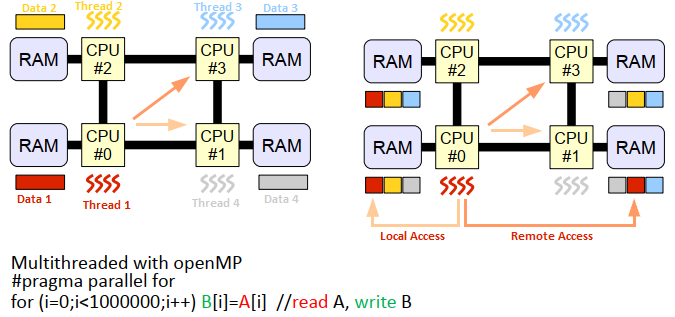
\includegraphics[scale=0.75]{num0091}
\centering
\caption{Exemples de placement des données du code OpenMP sur NUMA}
\label{fig:FG_2_num091}
\end{figure}
%
La proximité des threads à leurs données est cruciale pour la performance. 
Ceci est déterminé par les stratégies de placement du système d'exploitation et les modèles de programmation parallèle. Ces derniers souvent n'offrent aucun support explicite pour influencer le placement de la mémoire pour le programmeur.

Pour une mémoire partagée entre les processeurs à travers la plateforme avec des accès non uniformes, une distribution appropriée des données est nécessaire afin d'éviter les accès distants à la mémoire non locale. 
Les approches de la distribution des données sont :
%
\subsubsection{Round Robin}
%
En distribuant les données à tour de rôle entre les mémoires des nœuds. Elle est peu efficace et peut contribuer à amplifier l'effet NUMA en plaçant les données des threads sur des nœuds distants (aucune information n'est exploitée pour respecter l'affinité threads/données)
%
\subsubsection{Politique Affinity-on-First-Touch (AoFT)}
%
La plupart des plateformes NUMA implémentent cette première règle.
Si un thread demande un fragment de mémoire, le mappeur(qui exécute la politique de placement des données) s'assure que le fragment de mémoire est alloué à partir du segment de mémoire le plus proche à ce thread. %Elle est la plus facile à mettre en œuvre. 
La page mémoire contenant cette donnée est mappée dans le domaine local du processeur qui l'écrit en premier (c.-à-d. exécutant le thread qui a accédé à cette donnée). \cite{Mark11}
Solaris, Linux et Windows utilisent la stratégie dite de cette politique par défaut. 
Cela signifie qu'une page est placée dans la mémoire à côté du processeur à partir duquel le premier accès à la page se produit. 
Cette stratégie peut être exploitée dans une application en initialisant les données en parallèle dans le même schéma que celui auquel nous accédons pendant le calcul. 
%
\subsubsection{Politique Affinity-on-Next-Touch (AoNT)}
%
L'affinité next-touch est une autre approche pour réduire l'effet NUMA et maximi-ser l'affinité thread/données.
Lorsque l'ordonnanceur de système d'exploitation détecte qu'un processus accède à un bloc de mémoire qui ne se trouve pas dans le même nœud,
Il marque ce morceau de mémoire prêt à être déplacé.
Il essayera alors de trouver un moment approprié pour déplacer le morceau de mémoire vers le segment de mémoire approprié, qui est le plus proche du processus en cours. 
Selon Lankes et al. \cite {lak-pan} le système d'exploitation Sun / Oracle Solaris utilise la politique de distribution affinity-on-next-touch, alors que Linux n'a toujours pas cette fonctionnalité.

\textbf{Solaris} : Solaris propose l'appel système \textbf{madvise} via le MPO (optimisation du placement de la mémoire) installation, en prenant une plage d'adresses et un indicateur de modèle d'accès en tant qu'arguments. 
L'indicateur MADV ACCESS LWP indique au noyau que le prochain thread touchera la plage d'adresses spécifiée y accédera le plus fortement et pour déplacer les pages vers le noyau du thread accédant ou NUMA nœud, respectivement. 

\textbf{Linux} : Linux a un appel système supplémentaire \textbf{sys-move-pages} qui a été rendu disponible pour offrir des facilités de migration de page. 
En utilisant cette fonction, vous pouvez déplacer manuellement les pages d'un processeur à un autre. 
Mais l'application est toujours nécessaire pour savoir quel jeu de pages doit être déplacé vers quel processeur. 
En plus de cet appel système, l'outil \textbf{numactl} \cite{Linux13} peut être utilisé pour autoriser l'allocation de mémoire uniquement à partir d'un ensemble spécifié de nœuds NUMA, ou pour définir une politique d'entrelacement de mémoire. 
La mémoire sera ensuite allouée à l'aide d'une stratégie round-robin, qui peut améliorer les performances de l'application avec des modèles d'accès mémoire aléatoires. \cite{Dreb15}.

Löf et Holmgren \cite{HEN000} ont évalué une implémentation AFFINITY-ON-NEXT-TOUCH dans le mode utilisateur de sur un domaine isolé de 8 nœuds d'un Système Sun Fire 15000.
En utilisant AFFINITY-ON-NEXT-TOUCH, la performance est améliorée jusqu'à 166\%, ce qui montre ce placement de données peut avoir un impact énorme sur les performances des applications.

Goglin et Furmento \cite{GogFur09} ont implémenté AFFINITY-ON-NEXT-TOUCH pour le noyau Linux et ont comparé les performances à une implémentation de l'espace utilisateur. 
L'implémentation basée sur le noyau est environ 30\% plus rapide sur un système AMD Opteron 8347HE à quatre nœuds et affiche un surdébit significativement moins important que l'implémentation dans l'espace utilisateur pour les petites régions de mémoire. 
Cepen-dant, les auteurs concluent qu'une implémentation dans l'espace utilisateur fonctionne mieux dans les cas où des zones mémoire plus importantes utilisées par l'application doivent être migrées. 
L'implémentation mode noyau migre ces zones page par page, tandis qu'une implémentation mode utilisateur peut migrer chacune de ces zones en une seule opération avec une surcharge plus faible.
%
\subsection{Attâchement d'un Thread (Thread Binding)}
%
le système d'exploitation peut décider de déplacer un thread de son emplacement initial(\textbf{migration}). 
Cela peut entraîner une pénalité de performance, car les données du cache ainsi que la localité mémoire sont perdues. L'opération de la migration est coûteuse. 
Pour éviter cette migration, il est possible de \textbf{lier un thread} à un cœur donné ou à un sous-ensemble donné des cœurs d'un système. 
\textbf{Solaris} propose l'appel système \textbf{processor-bind()} pour lier un thread ou un ensemble de threads à un cœur spécifié. 
La fonction \textbf{sched-setaffinity()} de l'appel système \textbf{Linux} et l'appel de la fonction \textbf{SetThreadAffinityMask()} sur \textbf{Windows} s'attendent à ce qu'un masque de bits représentant les cœurs autorisés à l'exécution d'un thread spécifique. 
Une autre approche pour appliquer la liaison de thread est via des commandes spécifiques au système d'exploitation, par exemple. en utilisant la commande \textbf{taskset} ou les outils \textbf{numactl} sous \textbf{Linux} ou en appelant un programme avec \textbf{start /affinity} sur \textbf{Windows}. 
En utilisant ces outils, un processus peut être restreint à un sous-ensemble donné de cœurs de processeurs et tout thread créé par ce processus obéira à ces restrictions. 
%
\begin{table}[h!]
\centering
\begin{tabular}{| c | c | c | c | c | c | c |} 
\hline
Operating System    & AIX7.2    & FreeBSD11  & HP/UX  & Linux Arch4.1 & Solaris & Win10 \\ [0.5ex] \hline
Pin Thread             & +    & +  & +  & +  & +  & + \\ [0.5ex] \hline
Logical CPU/Node 	& +    & +  & +  & +  & +  & +  \\ [0.5ex] \hline
Mode distance        & -     & -   & -   & +   & -  & -  \\ [0.5ex] \hline
\end{tabular}
\caption{Fonctionnalités NUMA implémentées dans les systèmes d'exploitation courants} %
\label{table:TB_2_214}
\end{table}
%
La table \ref{table:TB_2_214} montre les fonctionnalités NUMA implémentées dans les systèmes d'exploitation courants.
%
%================================================================================
\newpage
\section{Conclusion}
%
Comme il n'était pas possible de continuer la course des fréquences pour les processeurs monocoeurs d'une part et les multiprocesseurs basés sur ces processeurs n'étaient pas assez puissants et soufrent de plusieurs limitations, alors multicœurs étaient une nouvelle direction pour continuer à exploiter les puissances des ordinateurs. Dans ce premier chapitre nous avons exposé les motivations de la révolution des multicœurs au début des années deux milles. En suite, nous avons présenté leurs caractéristiques et l'impact sur l'industrie logicielle (en adaptant les systèmes d'exploitation et les applications). Cette mutation a accéléré l'adoption des applications massivement parallèles par un grand nombre d'usager (développeur, scientifique,..). 
%
Les systèmes multiprocesseurs ont gagné de puissance en utilisant cette technologie, mais ils étaient pénalisés par un nombre de facteurs qui étaient intrinsèquement liés à leurs méthodes de conception classiques qui consistent à assembler les processeurs autours d'une mémoire partagée en utilisant un bus commun pour assurer l'équité de l'utilisation des ressources entre les processeurs (créant une symétrie et uniformité d'accès à la mémoire SMP/UMA). 
%
Cette utilisation intense a rapidement montré que nous ne pouvons pas continuer à concevoir les architectures parallèles avec un esprit classique (MC-SMP-UMA) vu qu'elle a exhibé des limites en donnant un niveau de performance loin de l'espéré. Un système de mémoire hiérarchique compliqué couplé à un système de communication utilisant un support partagé ont étaient les principaux facteurs responsables de la dégradation des performances (l'accès au bus partagé créant la contention de communication et limitant le passage à l'échelle, une mémoire assez lente par rapport le processeur). 
%
Le remplacement des bus par des réseaux de communication avec des mécanismes de routage d'une part et la distribution de la mémoire centrale entre les processeurs ont donné naissance à cette nouvelle conception des plateformes parallèles NUMA qui ne sont ni symétrique ni uniforme mais offrent plus d'avantages à ces applications massivement parallèles (passage à l'échelle).

Dans la partie consacrée à NUMA, nous avons décrit cette architecture en donnant ces principaux composants et comment elle contribue à surmonter le problème de passage à l'échelle des UMA. Par la suite nous avons parlé des spécificités/contraintes NUMA qui impactent grandement les politiques classiques d'ordonnancement des applications parallèles qui ne sont plus adaptées à ce contexte vu qu'elles ne sont pas concernées par la localité et le placement des données sur une mémoire distribuées et un espace d'adressage partagé. 
Alors nous avons présenté les modifications qui a été faite au système d'exploitation pour être adapté à NUMA (NUMA aware), en implémentant les politiques de placements des données standardisées ainsi que l'affinité des threads en les attachants à une unité d'exécution ou à un groupe d'unités.

Dans le chapitre suivant, nous allons parler des applications parallèles en générale et les applications parallèles décrites par un graphe de tâches en particulier.            
	\chapter{Graphes de tâches}
%
\newcommand{\RR}{\mathbb{R}}
\newcommand{\forto}{\text{\bf\ to\ }}
\newenvironment{defi}[1][Definition]{\begin{trivlist}
\item[\hskip \labelsep {\bfseries #1}]}{\end{trivlist}}
%
Dans ce chapitre, nous introduisons les concepts concernant la description des applica-tions parallèles à base de tâches en particulier les graphes de tâches, le modèle DAG et les modèles d'ordonnancement. Son objectif est de présenter les particularités structurelles de cette classe d'applications ainsi que son aspect fonctionnel lors de son ordonnancement et son exécution sur une plateforme multiprocesseurs.  

%Application parallèle décrite par DAG
Dans la section \ref{secAPdpDAG}, nous décrivons tout d’abord les applications à base de tâches ainsi que le graphe de tâches comme outils pour cette description.
%Modèle DAG
Ensuite dans la section \ref{modelDAG}, nous considérons le modèle DAG et nous présentons les concepts et la terminologie qui ont relation avec ce type de graphe. L'aspect dynamique résultant de son exécution sur une plateforme parallèle sera décrit en détail dans cette section.   
%Modèle d'ordonnancement
Les modèles d'ordonnancement ainsi que les algorithmes de résolution sont présentés dans la section \ref{modelSched}.
%Conclusion
Enfin la section \ref{concDAG} conclue ce chapitre.
%======================================================================================================
\section{Application parallèle décrite par DAG}\label{secAPdpDAG}
%
La parallélisation efficace d'une application nécessite une connaissance approfondie de la structure du programme. 
Il existe plusieurs méthodes pour déclarer la structure parallèle du programme à partir de sa version séquentielle en spécifiant les blocs (sections) séquentiels et leurs relations, souvent faite manuellement par le programmeur, 
Ces métho-des sont appelées les \textbf{modèles de la programmation parallèle}.
Comme exemples de ces modèles, on peut citer 
Fork-Join pattern \cite{ABB00}, les 
MPI (passage de messages) \cite{GLS99}, 
map-reduce pattern \cite{DG04}.
Ces modèles diffèrent dans leur API, dans leur granularité et leur fonctionnalité, 
ils partagent tous un objectif commun : 
partitionner le programme séquentiel et 
exécuter les blocs séquentiels résultants dans un ordre qui préserve leurs dépendances mutuelles sur la plateforme parallèle cible sur laquelle on exécute l'application (appelé \textbf{environnement d'exécution}).
La deuxième partie de ce processus (trouver cet ordre) s'appelle l'\textbf{ordonnancement}. 
Les blocs séquentiels représen-tent des parties du code séquentiel du programme sont appelés les \textbf{tâches}. 
L'environnement d'exécution matériel et logiciel où un algorithme ou l'application parallèle s'exécutent est appelé le \textbf{modèle de système}.
%
\subsection{Graphe de tâches}\label{ullmanNP}
%
Les dépendances entre les tâches représentent la relation fonctionnelle causale ou un partage de ressources ou de données (qui nécessitent d'être placées et transferées) entre les tâches concernées. Les données  utilisées par les tâches précédentes après leurs exécutions doivent être mises à jour et préparées pour les tâches suivantes. 
Ces relations de dépendance entre les tâches peuvent être modélisées en tant que graphe, et donc toutes les dépendances représentent une causalité de précédence temporelle ce qui empêche l'existence de tout cycle dans ce graphe (retour vers des tâches déjà exécutées) 
Ainsi, ce modèle s'appelle \textbf{Graphe acyclique dirigé (DAG)}.
%
%\begin{figure}
%\includegraphics[scale=0.75]{dag010}
%\centering
%\caption{Exemple d'une application parallèle décrite par un DAG}
%\label{fig:FG_3_1}
%\end{figure} 
%
%La figure \ref{fig:FG_3_1} montre un exemple d'un DAG qui modélise un programme parallèle. 
%
\begin{figure}
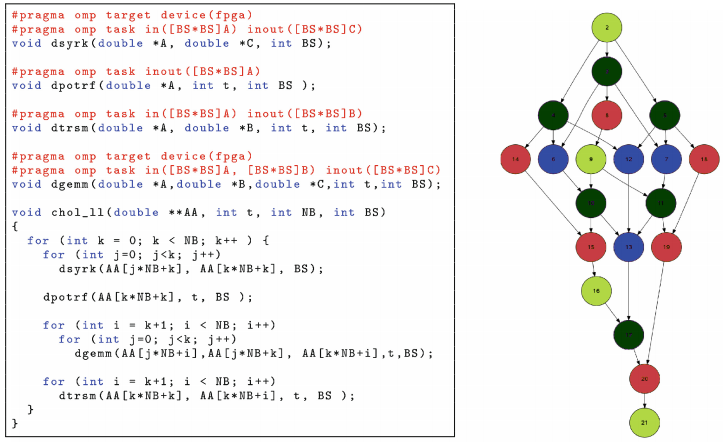
\includegraphics[scale=0.75]{dag011}
\centering
\caption{Exemple d'un code OpenMP parallèle et son DAG équivalent}
\label{fig:FG_3_1_0}
\end{figure} 
La figure \ref{fig:FG_3_1_0} montre un exemple d'un code OpenMP parallèle et son DAG équivalent.
%
Le problème de l'ordonnancement des programmes parallèles décrits par un DAG consiste à trouver l'ordre d'exécution (ressources temporelles) des tâches constituantes le programmes et sa projection sur la plateforme parallèle (ressources spatiales) de façon consistante qui respecte le principe de la causalité.
\textbf{Ullmann et al} ont montré que le \textbf{problème de l'ordonnancement d'un DAG sur une machine multiprocesseur} est un \textbf{problème NP-complet} sous sa forme générale \cite{Ull75}.
%
Les techniques d'ordonnancement les plus populaires ne tentent pas de trouver nécessairement un ordre optimal. 
Au lieu de cela, ils tentent d'en trouver un qui respecte leurs dépendances mutuelles et est en corrélation avec une métrique d'importance spécifiée qui favorise les tâches les plus importantes et les plus critiques pour l'exécution globale de l'application \cite{KA99}. 
La tâche de l'ordonnanceur ne dépend pas seulement de l'application parallèle à ordonnancer mais aussi de l'environnement de l'exécution.
%
Les techniques d'ordonnancement (algorithmes, politiques, stratégies) se caractérisent par la quantité d'informations et les détails à-propos du DAG exploitées pour réaliser son objectif.
Certains algorithmes utilisent peu d'informations sur la structure du programme dans ce processus 
(Certes une connaissance plus complète de la structure du programme, sa prise de décision peut devenir plus raisonnable et plus efficace, 
Mais en réalité beaucoup de ces informations ne sont pas disponibles lors de la conception (désigne-time) mais au moment d'exécution du programme (runtime)),  
Au lieu de cela, ils essaient d'utiliser des modèles qui donnent à un ordonnanceur une connaissance restreinte de la structure du programme lui permettant d'améliorer les performances dans un environnement d'exécution donné ce qui les rend plus rapides (atteindre une meilleure performance en ne connaissant qu'une partie de la structure du programme) \cite{HL14}.

Les propriétés de l'environnement où l'ordonnanceur agit ont une influence majeure sur la structure de l'algorithme d’ordonnancement. 
Selon que les processeurs soient ou non homogènes, quelle est la topologie de la plateforme, les informations sur le programme, etc., l'algorithme peut prendre ses décisions en considérant des informations très différentes. 
L'aspect principal est de savoir comment les propriétés de l'ordonnancement résultant dépendent de l'exhaustivité des informations disponibles pour l'algorithme. Le modèle de système se compose de trois composants : \\
%
- modèle plateforme\\
- modèle interconnexion\\
- modèle ordonnancement 

- \textbf{Le modèle plateforme} : décrit les propriétés des plateformes (processeurs, nœud de calcul,  ..), qui exécutent un programme parallèle et l’ordonnanceur lui-même. 
Les processeurs d'une plateforme peuvent être homogènes ou hétérogènes. 

- \textbf{Le modèle interconnexion} : décrit les propriétés des liens de communication qui connectent les processeurs et leur topologie.
Les liens de communication peuvent être une ressource partagée qui nécessitent une concurrence pour l'utiliser alors il faut gérer le conflit de ce partage dans ce contexte (avec conflit with-contention) ou être sans contention (contention-free). 
%
(Contestation-free, une fois qu'une opération de communication démarre, elle ne subit aucune perturbation par rapport à d'autres opérations de communication,
Cela signifie qu'une opération de communication occupe exclusivement le canal entre les deux processeurs et ne peut pas être interrompue). 

- \textbf{Le modèle ordonnancement} : décrit les informations disponibles pour un ordonnan-ceur et la manière dont son algorithme peut fonctionner avec ces informations disponibles.

Les algorithmes manipulant les graphes de tâche et générant les ordonnancement correspondants à une application décrite par ce modèle peuvent être divisés en deux classes suivantes :

1- \textbf{Algorithmes just-in-time (JIT-algorithmes)} 

Ces algorithmes ont très peu d'informations sur le programme pour lequel ils tentent de trouver un ordre d'exécution. 
Leurs décisions sont prises en runtime. 
Et la minimisation des coûts d'ordonnancement est souvent un objectif important pour eux. 

2- \textbf{Algorithmes complets}

Ces algorithmes connaissent la structure complexe du programme. %
Ils font chaque décision d'ordonnancement en tenant compte des répercussions possibles de l'avenir. 
Tout cela permet de réaliser toutes les actions nécessaires avant l'exécution de l'application, en temps de compilation (design-time). 
%===========================================================================
\section{Modèle DAG} \label{modelDAG}
%
L'exécution de programme parallèle se compose des tâches (code séquentiel), qui ont des dépendances de données entre elles. 
Une telle structure peut être modélisée selon un graphe dirigé acyclique (DAG), où 
les nœuds représentent des tâches (parties séquentielles) et 
des arcs (arêtes) représentent des dépendances de données. 
Divers paramè-tres du programme peuvent être modélisés soit comme attributs des nœuds, des arcs ou du graphe lui-même. 
%
\subsection{Concepts et définitions} 
%
Afin de montrer le processus de la description d'un code parallèle par un DAG, nous allons définir les concepts de base pour cette transformation et les notations utilisées par la suite. 
Nous commençons par la présentation d'un exemple de code séquentiel d'algorithme pour un problème classique du calcule numérique 'résolution d'un système d'équations dont la matrice est triangulaire' qui va servir de modèle.
  
Soit le problème de la résolution d'un système d'équation suivant : $A\cdot x=b$ \\
\begin{itemize}
    \item $A \in MTI_n(\RR)$ Matrice triangulaire inferieure donnée
    \item $b \in\RR^n$ vecteur constant
\end{itemize}

L'algorithme $AL001$ suivant calcule la solution de ce système :
%
\begin{algorithm}
  \caption{Résolution systeme d'équations}
  \DontPrintSemicolon
  \For{$i=1 \forto n$}{
	Task $T_{i,i}: x_i \gets \frac{b_i}{a_{i,i}}$\;
	\For{$j=i+1 \forto n$}{
	  Task $T_{i,j}: b_j \gets b_j - a_{i,j}x_i$
	}
  }
\end{algorithm}
%
Cet algorithme est séquentiel, la totalité du calcule est faite par les blocs de code (Tâche $T_{ij}$) de l'algorithme ou l'exécution de ces blocs suit un ordre total définit par la structure séquentielle du code.
%
\begin{définition}[Calculer Avant $<_{seq}$.]\textit{
%
On définit la relation d'\textbf{ordre total} sur $AL001$ \textbf{calculer avant} $<_{seq}$ :  
$$
T <_{seq} T'   \implies T \text{ est calculée / exécutée avant } T'
$$
%
}\end{définition}
%
On a l'ordre suivant pour les tâches de $AL001$ : $T_{1,1} <_{seq} T_{1,2} <_{seq} T_{1,3} <_{seq} \dots <_{seq} T_{1,n} <_{seq} T_{2,2} <_{seq} \dots <_{seq} T_{n,n}$

La logique de l'exécution des $T_{i,j}$ est la suivante : \\
- $T_{1,1}$ est la première tâche et calcule $x_1$, \\
- $T_{1,2}$ et $T_{1,3}$ utilisent $x_1$, elle doit attendre la fin de $T_{1,1}$ (calcul de $x_1$).\\
- $T_{1,2}$ met à jour $b_2$ et $T_{1;,3}$ met à jour $b_3$. $T_{1,2}$ et $T_{1,3}$ sont indépendantes et peuvent être exécutées dans n'importe quel ordre.

On caractérise la Tâche $T$ par :\\
- $In(T)$    : l'ensemble des variables lues par la tâche $T$.\\
- $Out(T)$  : l'ensemble des variables écrites par la tâche $T$.
%
\begin{définition}[Variables partagées.]\textit{
%
On définit l'ensemble $SV$ des \textbf{variables partagées} entre $T$ et $T'$ l'ensemble des variables qui peuvent être modifiées par les deux tâches ou une des tâches et lues par l'autre au cours de l'exécution. 
$$
SV(T,T') = ((Out(T) \cap Out(T')) \cup (Out(T) \cap In(T')) \cup (Out(T') \cap In(T))
$$
%
}\end{définition}
%
\begin{définition}[\textsc{Bernstein} conditions.]\textit{
%
$T$ et $T'$ sont \textbf{dépendantes}, si et seulement si elles partagent certaines variables à modifier $T \bot T'$.
%
$$
T \bot T' \iff SV(T,T') \neq \emptyset
$$
%
}\end{définition}
%\textbf{\textsc{Bernstein} conditions}
Dans l'exemple donné, on a $Out(T_{1,1}) \cap In(T_{1,2}) = \{x_1\}$ alors $T_{1,1} \bot T_{1,2}$ et $Out(T_{1,3}) \cap Out(T_{2,3}) = \{b_3\}$ alors $T_{1,3} \bot T_{2,3}$.

Si $T \bot T'$ alors elles doivent être ordonnées selon l'ordre de l'exécution séquentielle.
%
\begin{définition}[Relation de Précédence $\prec$.]\textit{
%
$T$ précède $T'$ si et seulement que $T$ et $T'$ partagent certaines variables et $T$ doit être exécuter avant $T'$ $T \prec T'$.
%
$$
T \prec T' \iff (T \bot T') \& T \leq_{seq} T'
$$
%
}\end{définition}
%Alors on a $T \prec T'$ $ \prec:= (<_{seq} \cap \bot)^+$
$\prec$: est un \textbf{ordre partial} (consistant avec $<_{seq}$): $< = (<_{seq} \cap \bot)^+$

Dans l'exemple, on a : 
$T_{2,4}$ et $T_{4,4}$: $T_{2,4}$ modifie $b_4$ et $T_{4,4}$ lit $b_4 \implies T_{2,4} \bot T_{4,4}; T_{2,3} < T_{4,4}$

$T_{4,4}$ et $T_{4,5}$: $T_{4,4}$ modifie $x_4$ et $T_{4,(}$ modifie $x_4 \implies T_{4,4} \bot T_{4,5}; T_{4,4} < T_{4,5}$

$T_{2,4}$ et $T_{4,5}$: $T_{2,4}$ et $T_{4,5}$ sont indépendantes 

\paragraph{Représentation par un graphe dirigé}
$G = (V,E)$\\
$V$ = ensemble de tâches.\\
$e=(T,T') \in E \iff T < T'$ relation de précédence $T$ est prédécesseur de $T'$
%
\begin{figure}  %[h]
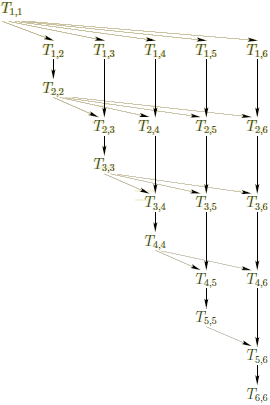
\includegraphics[scale=0.75]{dag006}
\centering
\caption{DAG de l'application résolution d'un système d'équations \cite{Dreb15}}
\label{fig:FG_3_2}
\end{figure} 
%
La figure \ref{fig:FG_3_2} montre le DAG correspondant au programme donné en exemple. 

Cette représentation donne un graphe dirigé et sans cycle appelé \textbf{graphe de précéden-ce} ou de \textbf{tâches  (DAG direct acyclic graph)} dont les nœuds sont des tâches (\textbf{calcul}) et les arcs représentent les dépendances entre les tâches (\textbf{communication}). 
Souvent cette description peut être complétée par les informations d'exécution (la durée de chaque tâche $w$, le volume des données échangées entre deux tâches communicantes $c$ si elles sont disponibles) dans certains cas DAG(T, <, w, c). 
Le coût de ce calcul et de cette communication ne dépend pas seulement de la durée des tâches et du volume échangé entre les tâches communicantes mais aussi des caractéristiques la plateforme sur laquelle elles s'exécutent.
C'est pourquoi il est important de caractériser et modéliser cette plateforme pour quantifier correctement les performances des politiques gérant l'exécution des applica-tions parallèles sur ces plateformes. La modélisation la plus simple est de représenter l'architecture cible par l'ensemble de ressources d'exécution (processeurs, cœurs, nœuds, ou autre) $\mathbb{P} = \{P_i\}_{i \in I}$ en donnant leurs caractéristiques.

Par la suite on va utiliser les fonctions suivantes :\\
- $\delta_\triangleleft(v_i)$ : \textbf{fonction prédécesseur} renvoie une liste des tâches qui précèdent la tâche $v_i$ (les tâches mères (nœuds parents prédécesseurs)).\\
- $\delta_\triangleright(v_i)$  : \textbf{fonction successeur} renvoie une liste des tâches dont l'exécution dépend de la tâche (du nœud) $v_i$ (tâches filles (successeurs)).\\
- $w(v_i)$ : \textbf{coût de calcul du travail} $v_i$.\\
- $c(e_{ij})$ : \textbf{coût de communication} $e_{ij}$ le volume des données échangées entre deux tâches.

Si les tâches $v_i$ et $v_j$ sont programmées pour le même processeur, alors $c(e_{ij}) = 0$. 
Sans perte de généralité, supposons qu'un DAG ait un seul nœud d'entrée et qu'un seul nœud de sortie. 
Tous les nœuds, à l'exception des nœuds d'entrée et de sortie, (initiaux et terminaux) ont des poids positifs $w(v_i) > 0$. 

Le \textbf{niveau statique sl} d'un nœud $v_i$ est la longueur du chemin le plus long du nœud $v_i$ au nœud de sortie, y compris le poids de $v_i$. 
S-level ne considère pas les coûts de communication, donc il ne dépend pas d'un ordonnancement particulier. 
%
$$
sl(v_i) = if(\delta_\triangleright(v_i) = \varnothing , 0 , \max_{ v_j \in \delta_\triangleright(v_i)}\{ sl(v_j) \} + w(v_i)
$$
%
Le \textbf{niveau statique supérieur (top) stl} d'un nœud $v_i$ est la longueur du chemin le plus long du nœud d'entrée vers un nœud $v_i$, à l'exclusion du poids de $v_i$. 
Le niveau statique supérieur inclut tous les coûts de communication et calculé avant l'établissement de l'ordonnancement. 
Ainsi, le calcul à un niveau ne considère pas la possibilité d'annuler les coûts de communication, lorsque des tâches dépendantes s'exécutent sur le même processeur. 
%
$$
stl(v_i) = if(\delta_\triangleleft(v_i) = \varnothing , 0 , \max_{ v_j \in \delta_\triangleleft(v_i)}\{ stl(v_j) + w(e_{ji})  + w(v_j) \}
$$
%
Le \textbf{niveau statique inférieur (bottom) sbl} d'un nœud $v_i$ est la longueur du chemin le plus long du nœud $v_i$ au nœud de sortie, y compris le poids de $v_i$. 
Le calcul du niveau b statique inclut les coûts de communication de la même manière qu'avec le niveau t. 
%
$$
sbl(v_i) = if(\delta_\triangleright(v_i) = \varnothing , 0 , \max_{ v_j \in \delta_\triangleright(v_i)}\{ sbl(v_j) + w(e_{ij}) \} + w(v_i)
$$
%
Le \textbf{travail total (W)} est la poids totale de toutes les tâches dans le DAG. 
Si toutes les tâches sont programmées sur le même processeur, la durée de l'ordonnancement résultant est égale au travail total. 
La formule pour calculer le travail total est la suivante :
%
$$
W = \sum_{ v_i \in V} w(v_i)
$$
%
Le \textbf{chemin critique (CP)} désigne la longueur du chemin le plus long du nœud d'entrée au nœud de sortie. 
Un DAG peut avoir plusieurs chemins critiques de même longueur. 
La longueur de chemin critique équivaut au niveau s d'un nœud d'entrée. 
Le chemin critique est un paramètre important d'un DAG, car il montre la limite inférieure de toute longueur de programme possible : 
Même avec une quantité illimitée d'exécution de processeurs ne peut pas prendre moins que l'exécution du chemin critique requiert. 
Le chemin critique peut également inclure les coûts de communication existant entre les nœuds dans le chemin critique. 

Les paramètres mentionnés ci-dessus ne dépendent pas d'un ordonnancement particulier qui peut affecter des tâches aux processeurs de manière différente. 
Ces paramèt-res sont appelés statiques. 
%
\subsection{Exécution  d'un DAG}  %3.1
%
Soit le DAG $G(V,E,w,c)$ qui décrit la structure d'une application parallèle que nous allons l'exécuter sur la plateforme de $m$ processeurs  $\mathbb{P} = \{P_i\}_{i \in [1..m]}$
%
\begin{définition}[Principe de causalité.]\textit{
%
L'ordonnancement d'un DAG $G(V,E,w,c)$ est la fonction $\theta$ qui associe à  chaque tâche sa \textbf{date début} : 
\begin{align*}
  \theta \colon V & \to \mathbb{R}\\
  v_i                    & \mapsto s_i = \theta(v_i).
\end{align*}
%
Vérifiant la relation (\textbf{principe de causalité}) :  
$$\forall (v_i, v_j) \in E, \theta(v_i) + w(v_i) < \theta(v_j)$$
%
}\end{définition}
%
Apres avoir déterminé un ordre chronologique de l'exécution des tâches d'un DAG, nous allons définir une fonction qui assure la projection des tâches sur les processeurs de la plateforme cible.
%
\begin{définition}[Principe de non chevauchement]\textit{
%
L'allocation d'un processeur à une tâche d'un DAG est la fonction $\pi$ qui associe à  chaque tâche un processeur sur lequel elle va être exécuté (renvoie un \textbf{processeur alloué} à la tâche $v_i$) : 
\begin{align*}
  \pi \colon V & \to \mathbb{P}\\
  v_i                    & \mapsto p_j = \pi(v_i).
\end{align*}
%
Vérifiant la relation (\textbf{principe de non chevauchement}) : 
$$\forall (v_i, v_j) \in V^2, \pi(v_i) = \pi(v_j) \equiv (\theta(v_i)+ w(v_i) < \theta(v_j)) or (\theta(v_j)+ w(v_j) < \theta(v_i))$$
%
}\end{définition}
%
Un \textbf{algorithme d'ordonnancement} détermine le début d'exécution et le processeur alloué d'une tâche. 

En donnant un ordonnancement particulier $\theta_k$, on peut déterminer les paramètres dynamiques suivants :

Le \textbf{temps de début} d'une tâche dans un ordonnancement particulier est désigné par $ ST(v_i) =  s_i $.

Le \textbf{temps de la fin} d'une tâche dans un ordonnancement particulier est désignée comme $ ET (v_i) = e_i $. 
Entre le début et la fin d'une tâche, on la relation suivante :  
%
$$
ET(v_i) = ST(v_i) + w(v_i)
$$
%
Le \textbf{temps total d'exécution (completion time, Makespan)} indique le temps de fin de la tâche de sortie. Aussi appelée durée de l'ordonnancement. note $C_{max}(\mathcal{O}_k)$

Le \textbf{niveau dynamique supérieur top} d'une tâche $v_i$ sur un processeur $P_j$ est la longueur du chemin le plus long de la tâche d'entrée vers la tâche $v_i$, à l'exclusion du poids de $v_i$. 
Ce niveau indique le temps de début le plus tôt possible d'une tâche $v_i$, lorsque les tâches antécédentes de $v_i$ est déjà ordonnancées.
%
$$
tl(v_i) = if(\delta_\triangleleft(v_i) = \varnothing , 0 , \max_{ v_j \in \delta_\triangleleft(v_i)}\{ FT(v_j) + w(e_{ji}) \}
$$
%
Le niveau t dynamique ne considère pas la disponibilité d'un processeur prêt pour exécution du nœud vi, donc le temps réel le plus tôt possible peut être plus grand.

Le \textbf{niveau dynamique inférieur bottom} d'une tâche $v_i$ sur un processeur $p_j$ est la longueur du chemin le plus long de $v_i$ à la sortie, y compris le poids de $v_i$. Ce niveau est calculé comme suit.
%
$$
bl(v_i) = if(\delta_\triangleright(v_i) = \varnothing , 0 , \max_{ v_j \in \delta_\triangleright(v_i)}\{ bl(v_j) + w(e_{ij}) \} + w(v_i)
$$
%
Le \textbf{temps prêt $RT(v_i, p_j)$} est le temps le plus tôt possible lorsque le processeur $p_j$ peut exécuter la tâche $v_i$. 

Le \textbf{temps début au plus tôt $EST(v_i,p_j)$} fait référence au temps d'exécution le plus tôt possible de la tâche $v_i$ sur un processeur $p_j$. 
%
$$
EST(v_i, p_j) = max \{ tl(v_i) , R(v_i, p_j) \}
$$
%
Le \textbf{premier temps de finition $EFT (v_i; p_j)$} se rapporte au temps de finition le plus tôt possible d'un nœud $v_i$ sur un processeur $p_j$. Entre EST et EFT suivant relation tient.
%
$$
EFT(v_i, p_j) = EST(v_i , p_j) + w(v_i)
$$
%
Le \textbf{temps de la fin réelle (AFT)} est le moment où la tâche achève son travail dans un ordonnancement particulier. 

Le \textbf{Temps début au plus tard (ALAP)} est une métrique qui indique combien le début d'une tâche peut être retardé sans augmenter le makespan. L'ALAP des tâches du chemin critique est égal à leur niveau t.

En donnant un $DAG$ et un environnement d'exécution $ENV$ et $\mathbb{O}$ soit l'ensemble de tous les ordonnancements possible de DAG sur $ENV$.

Un \textbf{problème d'ordonnancement $\Pi_{( \mathcal{O} | DAG, ENV)}$} consiste à déterminer l'\textbf{ordon-nancement optimal $\mathcal{O}^*$} de l'exécution de DAG sur ENV dont $C_{max}$ est le minimum.
%
$$
\mathcal{O}^* = arg \min_{ \mathcal{O}_i \in \mathbb{O}} \{  C_{max}(\mathcal{O}_i())   \} 
$$
%
Comme nous avons cité dans la section \ref{ullmanNP}, que \textbf{Ullmann et al} ont montré que le \textbf{problème de l'ordonnancement d'un DAG sur une machine multiprocesseur} est un \textbf{problème NP-complet} sous sa forme générale \cite{Ull75}. Trouver $\mathcal{O}^*$ généralement n'est assez facile. C'est pourquoi on cherche une bonne solution qui proche à la solution optimale avec un coût acceptable.
%---------------------------------------------------------------------------
Le listing suivant donne le contenu du ficher random000.stg selon le format StandardTaskGraph (STG) d'un DAG générique de 50 tâches et les figures suivantes \ref{fig:FG_3_1002} montre son ordonnancement sur les plateformes UMA de 4 cœurs et 8 cœurs respectivement.
%
\begin{Verbatim}[formatcom=\color{blue}]
#StandardTaskGraphSetProject
#RandomTaskGraph50//tmp/50/rand0000.stg
   50
   0   0   0
   1   9   1   0
   2   4   1   0
   3   3   1   0
   4   6   1   0
   5   4   1   1
   6   3   1   5
   7   3   1   0
   8   8   1   6
   9   9   1   0
   10    2   3   2   6   8
   11    1   1   9
   .............
   48   2   5   23   28   29   40   41
   49   9   4   30   39   46   47
   50   10   3    20   32   46
   51   0   11   3   17   31   34   38   42   43   45   48   49   50
\end{Verbatim}
%
\begin{figure}
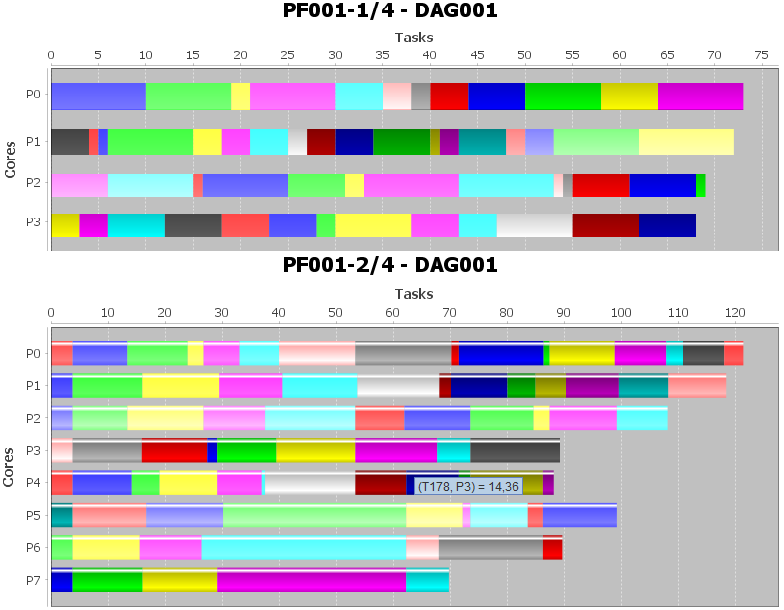
\includegraphics[scale=0.75]{dag10021}
\centering
\caption{Ordonnancement du DAG rand0000.stg sur des plateformes UMAs}
\label{fig:FG_3_1002}
\end{figure}
%===============================================================================
\newpage
\section{Modèle d'ordonnancement} \label{modelSched} 
%
Le modèle du système détermine la variété des algorithmes qui peuvent être utilisés. 
L'applicabilité du modèle est déterminée par les propriétés requises de l'environne-ment d'exécution. 
Des facteurs tels que les garanties de performance, la robustesse, la fiabilité et d'autres déterminent un modèle de système optimal et un algorithme d'ordonnancement optimal. 
Cette section présente des principes généraux d'ordonnancem-ent et des paradig-mes dans les modèles de système.
%
\subsection{Modèle Just-in-Time JIT}  
%
Le modèle Just-in-Time (JIT) ne prend pas en compte la structure du programme. 
Les ordonnanceur de ce modèle ne peuvent se permettre aucun ordre statique. 
On suppose qu'à chaque moment, un ordonnanceur connaît des informations très restreintes, mais cette information est à jour. 
Pour cette raison, les décisions de l'ordonnanceur doivent être prises immédiatement avant leur mise en œuvre, 

Dans le modèle just-in-time, les algorithmes d'ordonnancement des tâches DAG apparai-ssent pour l'ordonnanceur uniquement lorsqu’elles sont prêtes, i. e. toutes leurs dépendances sont satisfaites. 
Une tâche qui est en cours d'exécution sur un processeur est dite active. 
Si l'exécution d'une tâche dépend d'une autre tâche, alors la premiere est appelée une tâche-fille de la deuxième la tâche mère. 

Une queue globale et unique qui représente la file d'attente de tâches prêtes (dont l'état est prêt) est utilisée dans ce modèle. La tâche prête qui est en  entête de cette queue est affectée au processeur qui devient libre. 

Dans ce contexte, la contention pour le bus système peut diminuer drastiquement la latence et le débit du système \cite{ALL89} d'une part. 
D'autre part, L'influence de la localité des données sur le nombre de pertes de mémoire cache CPU \cite{HL14} et les défauts de page \cite{BLU96} participent à aggraver la situation. 
Cela augmente le trafic et la contenance du bus mémoire partagé et entraîne des pénalités de performance significatives. 

Si les tâches filles restent sur le même processeur que les tâches-mères, les pénalités de performance se développent plus lentement avec un nombre accru de processeurs \cite{SL93}.

\subsection{Horizon d'exécution pour les multicoeurs \cite{Pla15}}
L'ordonnancement est effectué en planifiant les tâches sur les processeurs disponib-les dans un ordre qui respecte les dépendances de données du DAG. 
%
Puisque initialement juste une information partielle sur l'application est disponible au support d'exécution, alors La prise de décision  se fait seulement au moment d'exécution de façon dynamique. 
Lorsqu'une application démarre, l'ordonnanceur découvre un certain nombre de tâches, à une certaine profondeur en fonction des tâches déjà traitées (soit complète, en exécution ou prête) ce qui constitue l'horizon d'exécution vu par l'ordonnanceur à ce moment. 
Certaines tâches sont prêtes à être exécutées juste après la fin de certaines tâches en exécution. Une fois qu'une tâche finit, l'ordonnanceur découvre ses descendants à une certaine profondeur et mis à jour l'horizon courant. Dans cet aspect, le modèle d'horizon est similaire au modèle JIT. Mais contrairement à ce dernier, l'ordonnanceur dans le modèle de l'horizon découvre plus d'informations après chaque étape d'exécution. Plus d'informations sur la structure de programme parallèle permettent à l’ordonnanceur qui permet de prendre une meilleure décision d'ordonnancement à chaque étape de l'exécution. 

Pour rendre cette information disponible, l'ordonnanceur peut utiliser les outils d'analy-se de code statique initialement pour extraction de certain aspect statique de l'application (sa structure, nombre des tâches,...) comme il peut utiliser les outils d'instru-mentation de l'exécution pour collecter les statistiques et les valeurs de certains paramètres après chaque événement d'exécution (la fin/début d'exécution d'une tâche, communication).

Les outils d'analyse de code statique devraient pouvoir reconnaître la structure de l'application (les parties séquentielles du programme et les dépendances entre eux). 
Le programmeur peut fournir certaines indications à ces outils en annotant le code source avec des directives dont l'interprétation par le compilateur permet de renseigner le support exécutif de certaines détails. 
En outre, l'outil d'analyse de code statique devrait pouvoir annoter l'image binaire du programme avec les informations sur ces parties séquentielles. 
Ces annotations devraient être reconnues par une partie dynamique d'un système parallèle, qui fournit un ordonnanceur avec une connaissance de l'horizon.
%
L'ordon-nanceur devrait pouvoir récupérer ces informations et l'utiliser pour prendre des décisions d'ordonnancement.
%
\subsection{Ordonnancement par liste}
%
Cette section décrit les détails de mise en œuvre qui sont souvent communs à tous ces modèles. 
Les algorithmes basés sur les heuristiques ne donnent pas une solution optimale, mais une solution proche de l'optimale. 
L'heuristique typique de l'algorithme de l'ordonnancement est appelée list scheduling \cite{KA99}. 
Le but des algorithmes de l'ordon-nancement de liste est de minimiser (ou maximiser) certains paramètres d'un programme résultant: makespan, équité, efficacité énergétique, 
il construit une liste de priorité de toutes les tâches dans le DAG en fonction de certaines métriques. 
Ensuite, l'ordonnanceur effectue une affectation des tâches aux processeurs dans l'ordre des priorités des tâches. 
Lorsqu'une tâche est affectée à un processeur, elle est supprimée de la liste des priorités. 
L'affectation peut avoir lieu 
soit de manière statique (avant l'exécution de l'exécution du programme), 
soit dynamiquement (pendant que le programme est en cours d'exécution). 
Si l'affectation a lieu pendant l'exécution, il peut se produire la situation suivante. 
Suppo-sons qu'un processeur est disponible pour l'exécution et que certaines tâches de la liste des priorités sont prêtes, 
mais la tâche la plus prioritaire n'est pas prête, car certaines dépendan-ces ne sont pas encore satisfaites. 
Cela peut se produire si la tâche supérieure de la file d'attente prioritaire dépend d'une tâche en cours d'exécution sur un processeur. 
Il y a deux solutions pour cette situation. 
Dans le premier, l'ordonnanceur attend que la tâche supérieure soit prête. 
Dans l'autre, l'ordonnanceur prend les tâches les plus prioritaires parmi les tâches prêtes. 
%
\subsubsection{Statique}
%
Les algorithmes de l'ordonnancement de listes statiques sont souvent combinés avec d'autres heuristiques de l'ordonnancement. 
L'algorithme de l'ordonnancement organise d'abord les tâches dans la liste des tâches. 
Cette liste a des tâches classées selon une certaine priorité. 
Le choix de la priorité dépend de l'algorithme et sa complexité de calcul varie, mais il est important de choisir la priorité de façon à ce que les tâches de la liste soient typologiquement triées. 
Si cette condition est remplie et si la file d'attente des tâches qui doivent encore être ordonnancées contient au moins une tâche prête, 
la tâche prête la plus prioritaire sera au sommet. 
Après la création d'une file d'attente de priorité des tâches, l'algorithme de l'ordonnancement se compose de deux étapes \cite{KA99}: 

1. Supprimer la tâche supérieure de la file d'attente de l'ordonnancement; 

2. Allouer la tâche à un processeur qui permet de l'exécuter le plus tôt possible. 

L'hypothèse initiale est que les tâches sont ordonnancées de manière à ce que chaque nouvelle tâche apparaisse à la fin de l’ordonnancement local d'un processeur. 
Il est simple à implémenter, mais peut être amélioré par insertion d’autres heuristiques \cite {KRU87}. 
%-----------------------------------
\IncMargin{1em}
\begin{algorithm}

\SetKwData{Left}{left}\SetKwData{This}{this}\SetKwData{Up}{up}
\SetKwFunction{Union}{Union}\SetKwFunction{FindCompress}{FindCompress}
\SetKwInOut{Input}{input}\SetKwInOut{Output}{output}
%
\Input{DAG G(Tasks,Edges); TopologyGraph TG(Nodes,Processors,Links)}
\Output{A schedule of G on TG}

\BlankLine   %\emph{special treatment of the first line}\;

$TasksList \gets sortTasksByPriority(Tasks)$ \;

\For{$each \text{ }  task \in TasksList$}{                               %	\emph{special treatment of the first element of line $i$}\;
	$processor \gets selectAvailableProcessor(task,Processors)$ \;
	$schedule(task, processor)$\;
}
%
\caption{Ordonnancement par liste statique}
\label{algo_static_scheduling}
\end{algorithm}
\DecMargin{1em}
%----------------------------------
\subsubsection{Dynamique}
%
Les algorithmes de l'ordonnancement de liste dynamique sont l'extension des algorith-mes de l'ordonnancement de listes statiques. 
Ils peuvent modifier la file d'attente prioritaire des travaux lors de sa construction. 
Cela se produit parce qu'après l'ajout d'une nouvelle tâche, la métrique utilisée pour affecter les priorités doit être recalculée pour toutes les tâches qui sont déjà dans la file d'attente prioritaire. 
Ainsi, un algorithme de l'ordonnance-ment de liste statique obtient une étape supplémentaire dans une construction de file d'attente prioritaire \cite{KA99}: \\
1. Déterminer les nouvelles priorités de toutes les tâches non ordonnancées\\
2. Sélectionner la tâche la priorité la plus élevée pour l’ordonnancement\\ 
3. Allouez la tâche au processeur qui autorise le plus tôt possible le début. 

L’ordonnancement dynamique a le potentiel de générer un meilleur ordonnancement que celui statique, mais comme inconvénient, il nécessite de recalculer en continu des priorités pour la file d'attente des tâches, augmentant ainsi la complexité temporelle de l'algorithme. 
%
\subsection{Par clustering}
%
Les heuristiques de clustering \cite{SIN08} supposent que le nombre de processeurs est effectivement illimité. Ainsi, l'objectif de minimiser le makespan est réduit au problème de l'optimisation des coûts de communication. Au début, Ces algorithmes attribuent à chaque tâche un processeur distinct. Dans le processus de recherche du meilleur ordonnan-cement un algorithme regroupe les clusters. La fusion des clusters signifie l'affectation des tâches de différents clusters au même processeur. Lorsque deux tâches, qui dépendent directement l'une de l'autre, sont mises sur le même cluster, les coûts de communication entre ces travaux deviennent nuls. Lorsqu'il y a un nombre de processeurs physiques supérieur au nombre de clusters, l'attribution de processeurs au cluster ne constitue pas un problème. Mais lorsque le nombre de clusters est supérieur au nombre de processeurs, une étape supplémentaire appelée mappage est nécessaire pour accomplir le processus de l'ordonnancement. Au cours de cette étape, un ordonnanceur doit mapper les clusters en processeurs physiques \cite{KA99}.
%
\subsection{Duplication des tâches}
%
L'heuristique de duplication a été présentée par Kruatrachue \cite{KRU87}. La duplication de tâches tente à réduire les frais de communication en clonant la tâche qui introduit une grande partie des coûts de communication. Ces tâches sont réparties entre plusieurs processeurs, de sorte que plus de communication se produit localement. Ainsi, l'heuristique de duplication de tâches tire parti du parallélisme et réduit les délais de communication en même temps.
%
\subsection{Basés les Metaheuristiques}
%
Les algorithmes déterministes ont un déséquilibre d'efficacité pour différentes configura-tions de workflow d'application parallèle. Avec très peu de chance, la dégradation des performances peut être significative. 

Les algorithmes basés sur les metaheuristiques tentent d'améliorer le processus de la recherche d'une solution au problème d'ordonnancement en introduisant la randomisation en écartant les solutions les moins efficaces. Différents types de ces algorithmes incluent :\\
- Algorithmes génétiques \cite{GRA99}\\ 
- Recherche Tabu\\
- Recuit simulé\\
- Colonie de fourmis

L'idée de ces algorithmes réside dans la génération de nombreuses solutions possibles et la sélection ultérieure des meilleures. Le processus de génération et de sélection est itératif. Typiquement, Cet algorithme commence par générer une solution aléatoire. Le nombre d'itérations de l'algorithme peut être volatile: l'algorithme s'exécute aussi longtemps qu'il est possible d'apporter une amélioration sensible. Ou il peut être fixé à un certain nombre constant. Comme pour les algorithmes déterministes, les algorithmes stochastiques dépen-dent fortement de la qualité des métriques utilisées pour comparer les solutions intermédiai-res et le processus de génération pour la prochaine génération. Parfois, un grand nombre d'itérations est nécessaire pour obtenir une solution de qualité acceptable.
%------------------------------------------------------------------------------------------
\newpage
\section{Conclusion}\label{concDAG}
%
Dans ce chapitre, nous avons parlé du deuxième aspect concernant cette thèse à savoir l'ordonnancement d'une application parallèle à base de tâches décrite par un graphe de tâches. 
%
Nous avons décrit tout d’abord les applications à base de tâches ainsi que le graphe de tâches comme outils pour cette description. Apres avoir partitionné la version séquentielle d'une application, nous obtenons un ensemble de tâche dont la granularité (la taille des tâches) dépend du niveau du processus de la parallélisation. L'étape suivante consiste à déterminer les dépendances entre les tâches qui une relation de causalité définit la précédence.
%
Le graphe résultant de ce processus est un DAG qui représente la structure de l'application avec les dépendances fonctionnelles et le partage de données/ressources. Les propriétés du DAG caractérisent la façon d'exécution sur une plateforme parallèle choisie en déterminant l'ordre temporel et spatial de cette dynamique. 
%

Pour cette fin, des modèles d'ordonnancement sont utilisés pour trouver l'ordre qui optimise cette exécution. Des algorithmes et des heuristiques spécifiques à chaque contexte sont conçus pour aider et faciliter la prise de décision.
%

Dans le chapitre suivant, Nous allons présenter l'état de l'art des problèmes d'ordonnan-cement des tâches et placement des données sur NUMA.
            
	\chapter{Etat de l'art de l'ordonnancement et le  placement sur MC-NUMA} \label{chapter:opdag} 
%
Dans ce chapitre, Nous allons présenter l'état de l'art des problèmes d'ordonnance-ment des tâches et placement des données dans le contexte de NUMA en exposant les différentes approches proposées durant cette décennie. Comme nous l'avons montré, la plateforme NUMA donne une solution au problème de la scalabilité de la plateforme UMA mais en contre partie elle introduit la pénalité NUMA due aux accès distants générés par le placement des données d'une tâche sur un nœud différent du nœud sur lequel elle s'exécute. Ce facteur a un impact important sur le processus d'ordonnancement et il contribue à rendre le temps total d'exécution assez important pour un DAG par rapport  %celui d'
une exécution sur une plateforme UMA.
La figure suivante \ref{fig:FG_2_dag1006} montre un ordonnancement du mème DAG sur les plateformes UMA (un noeud de 8 coeurs N1C8) et NUMA (avec 4 noueds de 2 coeurs chacun N4C2) respectivement.
%
\begin{figure}
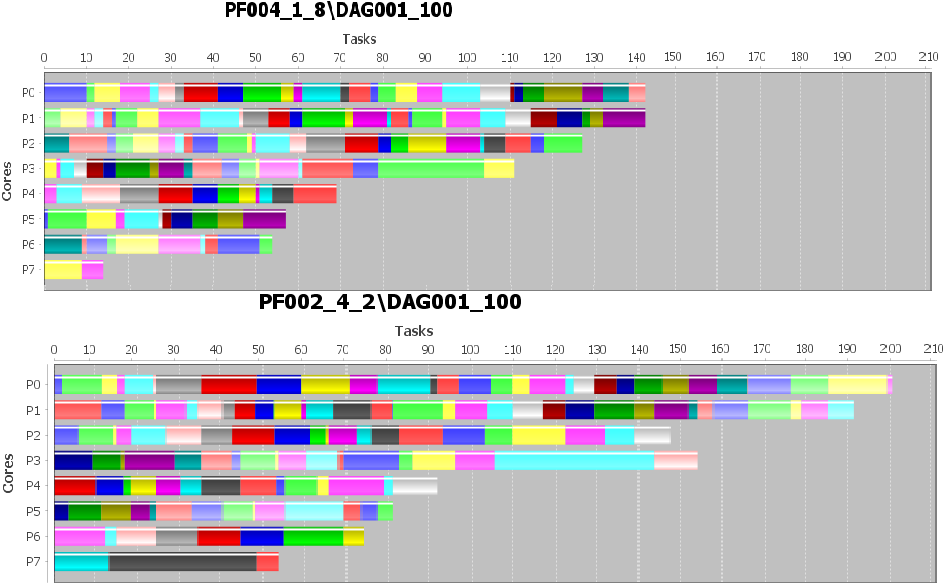
\includegraphics[scale=0.65]{dag1006}
\centering
\caption{Ordonnancement d'un DAG sur des plateformes UMA/NUMA}
\label{fig:FG_2_dag1006}
\end{figure}
%
Afin de réaliser l'objectif principal de l'ordonnancement et placement des données dans le contexte NUMA, les approches conçues ont été basé sur les idées qui exploitent certaines caractéristiques des architectures cibles \cite{Dreb15},
dont les principales caractéristiques sont les suivantes: \\  
- Les caractéristiques des applications ciblées par l'approche (parallélisation des boucles ou application régulière, irrégulière). \\
- L'ensemble des heuristiques (ordonnancement uniquement, placement uniquement ou les deux combinés). \\
- Le support logiciel d'implémentation (Système d'exploitation, Système d'exécution, Compilateur, Bibliothèque, Application ou une combinaison). \\
- Les informations utilisées et comment elles sont obtenues (indications de placement, affinités de données obtenues par profilage, Annotation du code source, ..).\\
- Le modèle de programmation cible (processus indépendants, fork-join \cite{FJ11} ,  OpenMP \cite{Omp00} \cite{Omp01} \cite{Omp02} ou Cilk \cite{Cil00} \cite{Cil01}).

La programmation parallèle des tâches est une approche de plus en plus populaire pour répondre aux attentes en matière d'évolutivité, et de productivité pour les applications destinées à fonctionner sur des systèmes à plusieurs cœurs. 
Les performances de l'exécution d'un tel type de programme dépendent fortement d'un système d'exécution optimisé capable d'exploiter efficacement le matériel sous-jacent. 
L'optimisation pour la hiérarchie de la mémoire, (caches et l'accès à la mémoire non uniforme), est un facteur clé dans ce contexte 
qui peut être réalisée grâce à un ordonnance-ment optimisé des tâches sur les cœurs et à un placement optimisé des données sur les contrôleurs de mémoire.   
Elle doit s'adapter à l'évolution rapide des architectures (nombre croissant des unités de calcul, réseaux d'interconnexion compliqué) et réagir aux changements dynamiques du comportement de l'application au moment de l'exécution pour équilibrer la charge.
Les approches peuvent être divisées en trois groupes \cite{Dreb15}\\
1- Aides à la prise de décision dont les informations sur les données pertinentes doivent être fournies par le programmeur.\\
2- Automatisant la prise de décision dont les informations fournies par le programmeur.\\
3- Automatisant la prise de décision et le recueil des informations sur les données pertinentes.

Les récents modèles de programmation parallèle à base de tâche tel que Cilk \cite{Cil00} \cite{Cil01}, OPENMP \cite{Omp00} \cite{Omp01} \cite{Omp02}, STARTS \cite{Sta00} et OPEN-STREAM \cite{Ost00} offrent de nouvelles opportunités au système d'exécution pour obtenir des informa-tions détaillées sur les données auxquelles accède une tâche ainsi que sur les dépendances inter-tâches. Ces modèles permettent de spécifier les dépendances inter-tâches en tant que dépendances de données et 
ainsi fournir au système d'exécution des informations précises sur les accès aux données par chaque tâche et le partage de données entre les tâches.

Dans la section \ref{caracAppro}, Nous présentons les grandes lignes des approches proposées en donnant les aspects qui caractérisent chaque classe. 
Ensuite la section \ref{ordoTKs} expose la première classe dont l'objectif principal est d'ordonnancer les tâches.
La deuxième classe qui focalise sur le placement est présentée dans la section \ref{placeDT}.
La section \ref{ordoPlaceComb} donne les approches qui combinent les deux aspects.
Comme l'équilibrage de charge est important pour préserver les performances, la section \ref{straECNUMA} est consacrée à détailler les stratégies utilisées pour cette fin.
Enfin la section \ref{concEdA} conclue le chapitre.\\
%=====================================================================================
\section{Caractéristiques des approches} \label{caracAppro}
L'étude des travaux connexes montre qu'il existe de nombreuses approches pour :\\ %différentes pour: \\
1- Améliorer la localisation des données par rapport à NUMA.\\
2- Réduire les conflits sur les contrôleurs de mémoire et sur les réseaux d’interconnexion.\\
3- Améliorer l'exploitation des caches grâce à un ordonnancement et un placement des données optimisées.

Le but de cette section est de donner une synthèse des approches avant de les exposer et de mettre en évidence les différences entre elles. 
Cette synthèse est divisée en trois parties. \\
\textbf{La première} : fournit un aperçu des caractéristiques générales. \\
\textbf{La deuxième} : se concentre sur les fonctionnalités liées au placement de données optimisé\\
\textbf{La troisième} : résume les caractéristiques des approches basée sur l'ordonnancement
%
\subsection{Caractéristiques principales}
Les caractéristiques générales des approches peuvent être résumées comme suit: \\
- La \textbf{partie de la hiérarchie de mémoire} optimisée par l'approche, c'est-à-dire si elle vise à améliorer les accès à la mémoire principale ou aux caches.\\ 
- La \textbf{couche de mise en œuvre} de l'approche (\textbf{IMP}) (par exemple, une bibliothèque (\textbf{LB}), le système d'exploitation (\textbf{OS}) ou le compilateur (\textbf{CP})).\\ 
- L'\textbf{infrastructure prise en charge} pour le parallélisme (par exemple, OpenMP, threads POSIX ou Cilk). \\
- La \textbf{technique} (\textbf{TCH}) sur laquelle est basée l'approche(sur un ordonnancement optimisée (\textbf{S}), un placement de données optimisé (\textbf{P}) ou si elle combine les deux techniques (\textbf{C})). 
%
\subsection{Caractéristiques du placement de données}
Les approches qui prennent en charge le placement de données diffèrent en ce qui concerne: \\
- \textbf{Source des données pertinentes SDP} : comment elles déterminent quelles données sont pertinentes pour améliorer le placement de données, en particulier si cela est fait automatiquement \textbf{A} ou si le programmeur \textbf{P} doit spécifier des structures de données pertinentes. \\
- \textbf{Les types de structures de données TSD} : quels types de structures de données sont supportés (par exemple, des tableaux ou toute région mémoire contiguë). \\
- \textbf{La granularité GRN} pour le placement de données (des éléments de données uniques, des pages ou des blocs représentant de grandes régions de mémoire). \\
- \textbf{Le moment de décision ToP} de placement est prise (par exemple, dynamiquement au moment de l'exécution, de manière statique au moment de la compilation ou pendant le profilage hors ligne). \\
%
\subsection{Caractéristiques des mécanismes d'ordonnancement}
Pour distinguer les approches de l'ordonnancement, nous avons identifié les caracté-ristiques suivantes: \\
- \textbf{Le type TYP} (par exemple, verrouillage de thread simple \textbf{THD}, ordonnancement de boucle \textbf{LOOP}). \\
- \textbf{La source des informations SID} sur lesquelles reposent les décisions (par exemple, les unités de surveillance des performances \textbf{SP}, les informations sur la distribution des données \textbf{DD} établies par l'approche elle-même ou le partage des données \textbf{SD} entre les threads).\\ 
- \textbf{Le type d'entités d'ordonnancement ENT} traitées par l'approche (par exemple, les threads du système d'exploitation, les itérations de boucle, les threads ou les tâches OpenMP). \\
- \textbf{Le moment de décision ToS} (par exemple, dynamiquement pendant l'exécution \textbf{EXE}, au début de l'exécution du programme \textbf{BEX} ou avant une boucle parallèle \textbf{BLP}).  
%=====================================================================================
\section{Ordonnancement des tâches}\label{ordoTKs}  %Scheduling and Mapping in MC-NUMA
%
Les approches suivantes reposent sur l'ordonnancement en tant que mécanisme princi-pal pour améliorer les performances des accès mémoire. 
\subsection{Principe de la réutilisation de l'ordonnancement}  
%
\textbf{1- Auteur}

Nikolopoulos et al. \cite{Nik01}.

\textbf{2- Idée}

Cette approche concerne la parallélisation des boucles. Elle prend en charge l'ordonnan-cement NUMA des itérations de boucle dans les applications OpenMP avec accès irrégulier à la mémoire principale. %Le premier exemple d'irrégularité géré par 
L'approche gère l'irrégularité des boucles imbriquées, où le bloc de l'itération de la boucle parallèle interne dépend de l'indice d'une boucle externe, de sorte que l'affectation des itérations de la boucle interne aux processeurs change entre itérations de la boucle externe. 
%
L'idée principale de l'approche est de distribuer d'abord les pages mémoires d'une structure de données accédée par une tâche (une boucle) sur des nœuds utilisant une description spécifique à l'application fournie par le programmeur par des annotations de code et de programmer des itérations des données sur les mêmes nœuds.
 
Le placement des pages est assuré par la politique first-touch qui place les pages de manière appropriée (sur le nœud de la première itération accédant à la structure de données). La localité de données est adressée en affectant des itérations suivantes accédant aux données aux processeurs associés aux nœuds contenant les données.

\textbf{3- Expérimentions}

La plateforme de l'expérimentation : c'est un système SGI Origin 2000 avec 64 proces-seurs regroupés en 32 nœuds.\\
Applications  :\\ 
1- \textbf{Décomposition de LU} (Application régulière), trois versions ont été comparé : \\
- une version OpenMP non modifiée. \\
- une version OpenMP modifiée avec des directives de distribution de données supportées par le compilateur SGI.\\
- l'approche SCHEDULE REUSE des auteurs.\\
\\
2- \textbf{Prévisions météorologiques} (Application irrégulière) deux variantes :\\
- Implémentés en utilisant OpenMP, avec l'approche SCHEDULE REUSE\\
- Avec le partitionnement de données explicite et le passage de message en utilisant MPI. 

\textbf{4-Evaluation}

L'approche de réutilisation de l'ordonnancement surpasse les deux versions d'Open-MP pour la décomposition de LU  
qu'elle surpasse les versions OpenMP non modifiées de l'Application de prévisions météorologiques et 
qu'elle offre des performances comparables aux Versions MPI.

\textbf{5- Commentaires}

La réutilisation de l'ordonnancement illustre que des informations statiques détail-lées sur les accès aux données, tirées du code source de l'application, peuvent être combinées avec une description d'une distribution de données spécifique à l'architecture pour une meilleure exploitation de la plateforme cible. 
%
\begin{center}%[htbp]
\begin{tabular}{l *{13}{l}} 		\hline
{TCH} & {IMP} 	& {SDP} 	&  {TSD} 	& {GRN} 	& {ToP} 	& {TYP} 	& {SPD}	& {ENT} 	& {ToS} \\     		\hline
C     	& CP+RT	& PRG		& ARY 	& ELT		& EXE		& LOOP	& DD 	  	& ITR 		& EXE    \\     		          \hline
\end{tabular}
 \captionof{table}{Caractéristiques de l'approche réutilisation de l'ordonnancement}% Add 'table' caption
\end{center} 
%
\subsection{Ordonnancement du parallélisme non structuré}\label{ordoPNS}
%
\textbf{1- Auteur}

Yoo et al. dans \cite{Yoo86}.

\textbf{2- Idée}

Le but de cette approche est d'optimiser les applications avec un parallélisme non structuré (c'est-à-dire des sections parallèles avec des tâches indépendantes qui peuvent être ordonnancées dans n'importe quel ordre avec une possibilité de partage des données). 
Les auteurs se sont concentrés sur les performances du cache en exécutant des tâches qui partagent des données sur des cœurs proches dans la hiérarchie de la mémoire. 

L'approche comprend trois parties principales. \\
- La première partie, la \textbf{charge de travail est profilée} afin de dériver des informations sur le partage de données entre les tâches. \\
- La deuxième partie consiste à \textbf{grouper des tâches}, à classer des groupes et à affecter les groupes à des files d'attente de travail associées aux composants de la hiérarchie de mémoire. \\
- La troisième partie traite de l'\textbf{équilibrage dynamique de la charge} grâce à un détournement de tâche sensible à la localité. 

Le résultat de l'exécution du profilage est un graphe de partage de tâches dont les sommets représentent des tâches et dont les arcs non dirigés capturent les relations de partage de données entre les tâches. 
Le poids associé à une arête indique le nombre de lignes de cache accessibles par les deux tâches connectées par un arc. 
Le graphe est ensuite partitionné de manière heuristique et récursive en groupes pour chaque niveau de la hiérarchie de mémoire, en commençant par le cache de dernier niveau. 
Chaque groupe de tâches est choisi de sorte que l'ensemble de travail des tâches s'insère dans un cache du niveau ciblé dans la hiérarchie de mémoire et de sorte que le partage de données intra-groupe soit maximisé. 
Le résultat est une hiérarchie de groupes de tâches qui peuvent être ordonnancées sur les files d'attente associées à chaque composant de la hiérarchie de mémoire, 
%
Au moment de l'exécution, les tâches sont exécutées par des \textbf{threads de travail (worker)} avec un thread par cœur. 
Lorsqu'un thread (worker) a fini d'exécuter une tâche, il essaie d'abord d'obtenir une tâche de sa file d'attente locale associée à son cache de premier niveau.
Si cette file d'attente est vide, le worker tente de prendre des tâches de l'une des files d'attente associées au cache de premier niveau de ses cœurs voisins par rapport au niveau suivant dans la hiérarchie de mémoire. 
Si ces files d'attente sont également vides, le worker tente d'obtenir un groupe de tâches à partir de la file d'attente associée à son cache de deuxième niveau. 

\textbf{3- Expérimentation}

Cette approche a été appliquée sur les charges de travail générales (base de données, reconstruction d'image 3D, détection de collision, traitement d'image, multiplica-tion matricielle et solveur pour équations aux dérivées partielles).

\textbf{4- Evaluation}  

Le groupement de tâches, le classement et l'assignation aux files d'attente, mais sans vol de travail sensible à la localité, peuvent accélérer l'exécution de 2:39 sur 32 cœurs pour les tests de mémoire intensifs et jusqu'à 3:57 sur 1024 cœurs. 
Le vol de travail sensible à la localisation sur 32 cœurs peut accélérer l'exécution de 1:9 par rapport à un vol de travail aléatoire avec un déséquilibre de charge créé par un nombre de workers inférieur au nombre de cœurs. 

\textbf{5- Commentaires}

L'approche montre que l'exploitation du partage de données dans l'ordonnanceur peut conduire à des améliorations de performances significatives. 
Elle illustre également que l'affectation initiale des tâches peut être combinée avec une technique de vols de travail tenant compte de la localité pour l'équilibrage de charge qui réagit aux circonstances au moment de l'exécution. L’approche du parallélisme non structuré ne fournit aucune forme de placement de données explicite. 
%
\begin{center}%[htbp]
\begin{tabular}{l *{13}{l}} 		\hline
{TCH} & {IMP} 	& {SDP} 	&  {TSD} 	& {GRN} 	& {ToP} 	& {TYP} 	& {SPD}	& {ENT} 	& {ToS} \\     		\hline
S     	& RT		& -		& - 		& -		& EXE		& TASK	& DS 	  	& TASK 	& SoX    \\     		          \hline
\end{tabular}
 \captionof{table}{Caractéristiques de l'Ordonnancement du parallélisme non structuré}% Add 'table' caption
\end{center} 
%=====================================================================================
\section{Placement des données} \label{placeDT}
%
Dans cette section nous allons donner les différentes approches pour le placement des données.
%
\subsection{Affinity on touch AoT}
%
\textbf{1- Auteur}

L. Henrik et al. \cite{HEN000}, \cite{AffOnNextTouch}.

\textbf{2- Idée}

De nombreux systèmes d'exploitation utilisent le placement \textbf{AFFINITY-ON-FIRST -TOUCH (AoFT)} comme stratégie de placement par défaut, dans laquelle une \textit{page de mémoire physique est allouée sur le nœud associé à la tâche qui écrit en premier sur la page ou lit la page}. 
Si les cœurs qui initialisent les structures de données et ceux qui y accèdent se trouvent sur le même nœud, l'AoFT génère une forte densité d'accès mémoire local. 
Cependant, si les nœuds d'initialisation et les nœuds d'accès ne correspondent pas, cette stratégie peut entraîner un conflit élevé et une forte proportion d'accès à la mémoire distante.
 Une stratégie courante pour contourner ce problème consiste à \textit{migrer dynamiquement les pages après l'initialisation vers les nœuds qui effectuent les accès en écriture suivants}. 
Cette stratégie, appelée \textbf{AFFINITY-ON-NEXT-TOUCH (AoNT) ou MIGRATE-ON-NEXT-TOUCH}, peut être entièrement implémentée dans l'espace utilisateur en utilisant des appels système pour la protection mémoire et la migration de page synchrone ou dans l'espace noyau pour la migration transparente et asynchrone. 

\textbf{3- Expérimentation}

Löf et Holmgren \cite{HEN000} ont évalué une implémentation d'espace utilisateur de AoNT sur un domaine isolé de 8 nœuds d'un système Sun Fire 15000 exécutant une application calculant la diffusion d'ondes électromagnétiques dans un espace tridimensionnel principa-lement pour résoudre un ensemble d'équations en utilisant la méthode du gradient conjugué. Goglin et Furmento \cite{GF50} ont implémenté AoNT pour le noyau Linux sur un système AMD Opteron 8347HE à quatre nœuds.

\textbf{4- Evaluation}

En utilisant AoNT, la performance est améliorée jusqu'à 166\%, ce qui montre que le placement de données peut avoir un impact énorme sur les performances de l'application. 
Pour Goglin et Furmento \cite{GF50} ont comparé les performances à une implémentation d'espace utilisateur. 
L'implémentation basée sur le noyau est environ 30\% plus rapide et affiche un sur débit significativement moins important que l'implémentation de l'espace utilisateur pour les petites régions de mémoire. 

\textbf{5- Commentaires}

Les auteurs concluent qu'une implémentation de l'espace utilisateur est plus performan-te dans les cas où de plus grandes zones de mémoire connues par l'application doivent être migrées. 
L'implémentation d'espace noyau migre ces zones page par page, tandis qu'une implémentation d'espace utilisateur peut migrer chacune de ces zones en une seule opération avec une surcharge plus faible.
Cependant, il appartient au programmeur ou à un composant logiciel de niveau supérieur de déclencher la migration de la page. 
%
\begin{center}%[htbp]
\begin{tabular}{l *{13}{l}} 		\hline
{TCH} & {IMP} 	& {SDP} 	&  {TSD} 	& {GRN} 	& {ToP} 	& {TYP} 	& {SPD}	& {ENT} 	& {ToS} \\     		\hline
P     	& OS-LB	& PRG-PFL	& - 		& PG		& EXE		& - 	  	& - 		& -    		& -\\     		          \hline
\end{tabular}
 \captionof{table}{Caractéristiques de l'Affinity on Touch}
\end{center}
%
\subsection{CARREFOUR} 

\textbf{1- Auteur}

Dashti et. al \cite{Das44}.

\textbf{2- Idée}

C'est un mécanisme de placement de données compatible NUMA pour le noyau Linux.  
CARREFOUR essaie d'éviter la congestion sur les contrôleurs de mémoire et les liens d'interconnexion et 
considère la réduction de la latence des accès mémoire en améliorant la localisation des données uniquement comme objectif secondaire. 
L'approche est basée sur quatre techniques: \\
1- La \textbf{co-localisation de pages} : il place une page sur le même nœud que le cœur accédant\\
2- L'\textbf{entrelacement de pages} : il place les pages sur des nœuds de manière circulaire\\
3- La \textbf{réplication de page} : il réplique des pages sur plusieurs nœuds\\
4- Le \textbf{clustering co-programme} : il place les threads en fonction de leur intensité de partage de données. 

La combinaison de ces techniques et l'application de chaque technique dépendent du comportement des applications exécutées sur la machine. 
Cela implique \\
- des décisions globales qui activent ou désactivent des techniques individuelles globalement\\
- des décisions page-locales qui activent ou désactivent des techniques par page. \\
Les statistiques qui servent de base pour caractériser le comportement du programme sont dérivées des valeurs fournies par un composant de mesure qui utilise \textbf{INSTRUCTION-BASED SAMPLING (IBS)} \cite{IBS48}.

Les décisions globales sont prises en quatre étapes. Dans :

1- La première étape, le système décide si le placement de données est nécessaire ou non. 
À cette fin, CARREFOUR compare le nombre d'accès mémoire par unité de temps du système entier à un seuil déterminé expérimentalement de 50 accès par microseconde. 
Si la valeur réelle de l'application est inférieure au seuil, CARREFOUR est désactivé et aucune autre action n'est entreprise. 

2- La deuxième étape consiste à décider si la réplication de page doit être activée ou désactivée. 
Pour éviter une charge de synchronisation élevée en raison des mises à jour fréquentes du contenu des pages, la réplication de page est uniquement utilisée pour les applications dont la fraction d'accès en lecture à la mémoire DRAM est supérieure à 95\%. 

3- La troisième étape, CARREFOUR vérifie si l'entrelacement doit être utilisé pour distribuer les demandes à la mémoire principale à tous les contrôleurs de mémoire. 
Cette décision est basée sur le déséquilibre du contrôleur de mémoire, qui est défini comme l'écart-type de la fréquence des accès mémoire entre les nœuds. 
L'entrelacement n'est appliqué que si la valeur est supérieure à un seuil de 35\%. 

4- La co-localisation est activée pour les applications dont le taux d'accès local est inférieur à 80\%, c'est-à-dire que la fraction des accès mémoire qui cible un nœud local est inférieure à 80\%. 
Les décisions locales-locales sont prises individuellement pour chaque page en analysant les statistiques dérivées des échantillons IBS qui appartiennent aux instructions d'accès à la page. 
Une page est migrée vers un nœud si la migration de page est activée globalement et si la page n'est accessible que par les cœurs d'un seul nœud. 
La réplication de page se déclenche si le mécanisme est autorisé globalement et si la page n'a été consultée qu'en lisant les instructions.
Une page accessible par des cœurs de plusieurs nœuds en mode lecture et écriture est placée en utilisant le mécanisme d'entrelacement qui déplace la page sur le nœud avec le plus petit nombre d'accès mémoire par unité de temps afin de réduire les conflits. 

\textbf{3- Expérimentation}

L'évaluation expérimentale de CARREFOUR a été réalisée sur deux machines systèmes AMD Opteron à 16 et 24 cœurs respectivement, regroupées en quatre nœuds. 
Les applications utilisées pour cette évaluation sont la suite PARSEC BENCHMARK (version 2.1), le moteur de reconnaissance faciale FACEREC (version 5.0).
Les performances de CARREFOUR ont été comparées à la stratégie par défaut de mise en page de First-touch du noyau Linux, entrelacement sur tous les nœuds.

\textbf{5- Evaluation} 

CARREFOUR fonctionne nettement mieux que le placement de pages par défaut (jusqu'à 3:63 plus rapide). 
Comparé à l'entrelacement sur tous les nœuds, CARREFOUR améliore significativement la performance dans la plupart des cas et 
limite la dégradation des performances dans les cas où l'entrelacement entre tous les nœuds dégrade les perform-ances par rapport au positionnement par défaut du système d'exploitation. 

\textbf{5- Commentaires}

CARREFOUR ne parvient pas à améliorer les performances des applications avec des changements de comportement rapides en raison de la précision d'échantillonnage limitée nécessaire pour un échantillonnage à faible débit. 
CARREFOUR montre que la contention est un problème important sur les systèmes NUMA car les optimisations qui diminuent les contentions entraînent une amélioration significative du temps d'exécution. 
%
\begin{center}%[htbp]
\begin{tabular}{l *{13}{l}} 		\hline
{TCH} & {IMP} 	& {SDP} 	&  {TSD} 	& {GRN} 	& {ToP} 	& {TYP} 	& {SPD}	& {ENT} 	& {ToS} \\     		\hline
C     	& OS		& PFL		&  - 		& PG		& EXE		& THD CLS	& OS 		& OS THD  & EXE  \\     		          \hline
\end{tabular}
 \captionof{table}{Caractéristiques de l'approche CARREFOUR}% Add 'table' caption
\end{center}
%
\subsection{Interface memory affinity MAI}    %Thread pinning    	& -      		& PThreads    	& Start of execution      & -\\\lipsum 

\textbf{1- Auteur}

C. Pousa RibeiroDashti et. al \cite{MAI77}.

\textbf{2- Idée}

C' est une interface de placement de données dont l'implémentation fournit un certain nombre de politiques pour la distribution des pages d'un tableau:\\
1- \textbf{bind\_all} : place toutes les pages sur un seul nœud et ne passe pas à d'autres nœuds que si toute la mémoire du nœud actuel est en cours d'utilisation.\\
2- \textbf{bind\_block} : divise d'abord le tableau en blocs, puis place chaque bloc sur un nœud différent.\\ 
3- \textbf{cyclique} : distribue les pages d'un tableau de manière circulaire sur tous les nœuds de la machine, de telle sorte que la i$^{ième}$ page est placée sur le nœud dont l'identifiant est \textbf{i mod M}, \textbf{M} étant le nombre de nœuds. \\
4- \textbf{cyclic\_block} : distribue des blocs de pages suivantes sur des nœuds de manière circulaire.\\
5- \textbf{\_mapp} : combine deux politiques: d'abord, il associe des pages à $P$ blocs de données virtuels en utilisant la politique cyclique. La deuxième étape consiste à redistribuer les blocs virtuels aux nœuds en utilisant à nouveau la politique cyclique. \\
6- \textbf{random} : elle place les pages de manière aléatoire entre les nœuds. 

\textbf{3- Expérimentation}.

L'évaluation de MAI a été réalisée sur des systèmes à quatre et huit nœuds NUMA pour les applications FFT et CG de la version OpenMP du NAS PARALLEL BENCHMA-RKS ainsi que pour une implémentation OpenMP d'une application géophysique.

\textbf{4- Evaluation}. 

Les stratégies proposées par MAI peuvent améliorer les performances de jusqu'à 31\% par rapport à la stratégie d’AoFT par défaut du système d'exploitation, mais doivent être choisies manuellement. 

\textbf{5- Commentaires}

Les auteurs ont conclu que la meilleure stratégie pour le placement de données dépend de l'architecture cible ainsi que de la structure des accès mémoire. 
Les machines avec une grande différence entre la latence des accès locaux et distants bénéficient d'un placement de données optimisé pour la localité, comme bind\_block, 
tandis que l'exécution sur des machines avec une faible différence entre ces latences peut être améliorée avec un placement qui améliore la répartition cyclique, aléatoire. 
Les applications avec une affinité claire des calculs et des données donnent des performances plus élevées avec bind\_block et 
les applications avec des accès irréguliers bénéficient de la distribution des données sur les nœuds. 

Les résultats présentés dans l'évaluation expérimentale de MAI montrent que le compo-rtement d'une application nécessite différents types de distributions de données aux nœuds et souligne que l'architecture joue également un rôle important dans la sélection d'une stratégie de placement.
%
\begin{center}%[htbp]
\begin{tabular}{l *{13}{l}} 		\hline
{TCH} & {IMP} 	& {SDP} 	&  {TSD} 	& {GRN} 	& {ToP} 	& {TYP} 	& {SPD}	& {ENT} 	& {ToS} \\     		\hline
P     	& LB		& PRG		&  ARY 	& BL/PG	& EXE		& THD PIN	& - 		& PTH   	& SOX  \\     		          \hline
\end{tabular}
 \captionof{table}{Caractéristiques de l'approche MAI}% Add 'table' caption
\end{center}
%
\subsection{MINAS}

\textbf{1- Auteur}

C. Pousa RibeiroDashti et. al \cite{MINAS76}.

\textbf{2- Idée}

MINAS combine les capacités de placement de données de MAI avec un préproces-seur appelé MAPP et NUMARCH, un module qui fournit des informations sur l'architecture cible. 
MAPP traite le code source d'une application, trouve des tableaux statiques partagés et remplace leurs déclarations par des appels appropriés aux fonctions d'allocation et de distribution de mémoire de MAI. 
La politique réelle pour la distribution de données choisie par MAPP dépend des caractéristiques de la plate-forme NUMA signalée par NUMARCH. 
Pour les systèmes ayant une latence d'accès distant élevée par rapport à la latence des accès locaux, la politique bind\_block est choisie afin d'optimiser la latence. 
Sur les systèmes avec une latence d'accès à distance inférieure, le framework optimise la bande passante et utilise la politique cyclique. 

L'approche utilise deux métriques pour caractériser la communication : \\
1- la première est basée sur la quantité de mémoire accessible par deux threads \\
2- la seconde mesure le nombre d'accès aux blocs de mémoire partagée. 

\textbf{3- Expérimentation}.

L'évaluation expérimentale a été réalisée sur un système AMD Opteron 875 avec 8 nœuds NUMA et 16 cœurs au total, ainsi que sur un système Intel Xeon X7560 avec 4 nœuds NUMA et 32 cœurs au total. 
Les performances de l'optimisation automatique avec MINAS sont comparées à la politique de placement de pages par défaut du système d'exploitation ainsi qu'aux versions des applications réglées manuellement en utilisant des combinaisons de stratégies de distribution correspondant le mieux aux modèles d'accès aux données. 
Les applications utilisées pour l'évalua-tion sont les mêmes que pour l'évaluation de MAI avec un benchmark supplémentaire qui simule la propagation des ondes en trois dimensions. 
%Une autre évaluation où l'application est exécutée dans un simulateur de système complet ses accès mémoire sont enregistrés dans un fichier de trace qui sera analysé afin de générer des matrices de partage qui indiquent pour chaque paire de threads comment intensément ces threads communiquent.

\textbf{4- Evaluation}. 

La solution automatique améliore les performances par rapport à la stratégie de positionnement de page par défaut du système d'exploitation, mais reste derrière les performances des codes réglés manuellement. 
La différence entre les versions automatique et manuelle varie de 0\% à 25\%. 

Les auteurs ont montré que pour les mappages de threads et de données basés sur la matrice de partage, des améliorations significatives du temps d'exécution allant jusqu'à 75\% peuvent être réalisées par rapport au mappage de thread et de données par défaut du système d'exploitation. 

\textbf{5- Commentaires}

%Les résultats montrent que, 
Bien que l'approche automatique ne puisse pas correspondre aux performances du code réglé manuellement dans certain cas.
L'approche montre que le profilage peut être utilisé pour obtenir des informations détaillées sur les échanges de données entre threads, ce qui peut être exploité pour améliorer le positionnement des applications avec des modèles distincts pour les accès mémoire.
%
\begin{figure}[h]
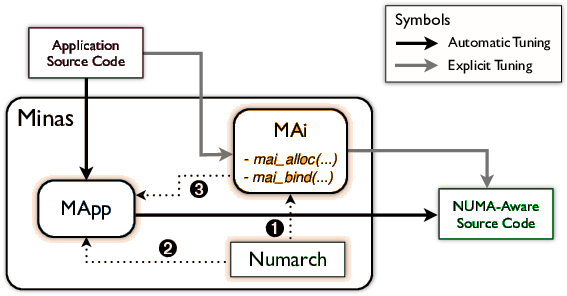
\includegraphics[scale=0.75]{Minas001}
\centering
\caption{MINAS Framework}
\label{fig:mci7}
\end{figure}   %\lipsum 
%
\begin{center}%[htbp]
\begin{tabular}{l *{13}{l}} 		\hline
{TCH} & {IMP} 	& {SDP} 	&  {TSD} 	& {GRN} 	& {ToP} 	& {TYP} 	& {SPD}	& {ENT} 	& {ToS} \\     		\hline
C     	& PP+LB	& PPR		&  ARY		& BL/PG	& EXE		& CoSCH	& DS 		& PTHD 	& SOX  \\     		          \hline
\end{tabular}
 \captionof{table}{Caractéristiques de l'approche MINAS}
\end{center}
%
\subsection{Placement de pages orienté feedback FBoPP}  % pour OpenMP FdP 
%
\textbf{1- Auteur}

Marathe et al \cite{Mar62}.

\textbf{2- Idée}

C'est un placement guidé par la trace de pages pour les programmes OpenMP. 
L'appro-che est divisée en trois phases:

a- \textbf{La génération de traces}\\
Pendant la génération de trace, le framework exécute une version tronquée du programme dont le placement de données doit être amélioré. 
il présente des informations détaillées sur les accès mémoire et les allocations de mémoire en utilisant les outils pour enregistrer les performances des processeurs et 
en interceptant les appels à l'allocateur de mémoire de la bibliothèque d'exécution C / FORTRAN. 

b- \textbf{La décision d'affinité}\\
Les décisions d'affinité consistent à déterminer sur quel nœud chaque page doit être placée, en fonction des accès de la trace. 
Le framework fournit un modèle simple, dans lequel la latence d'un accès à distance est supposée être indépendante de la distance entre le cœur demandeur et le nœud qui satisfait la demande. Dans ce modèle, une page est associée au nœud ayant le plus grand nombre d'accès à la page. Ainsi qu'un modèle plus sophistiqué qui prend en compte des latences variables. 

c- \textbf{Le placement de pages guidées par trace}\\
Le placement de page réel est effectué lors de l'exécution du programme entier en intercep-tant les appels à l'allocateur de mémoire et en initialisant des pages sur le nœud approprié avant de transmettre les régions de mémoire à l'application. 

\textbf{3- Expérimentation}\\
Les auteurs ont testé cette approche sur les applications de la version C du NAS PARALLEL BENCHMARKS et des applications des benchmarks SPEC OMPM2001 sur un système NUMA avec quatre nœuds.

\textbf{4- Evaluation}\\
le nombre d'accès mémoire distants et le temps d'exécution peut être diminué de manière significative . 

\textbf{5- Commentaires}\\
Le placement de pages orienté feedback est une approche qui exploite les informations obtenues par le biais du profilage pour améliorer le placement des données. 
%
\begin{center}%[htbp]
\begin{tabular}{l *{13}{l}} 		\hline
{TCH} & {IMP} 	& {SDP} 	&  {TSD} 	& {GRN} 	& {ToP} 	& {TYP} 	& {SPD}	& {ENT} 	& {ToS} \\     		\hline
C     	& OS		& PFL		&  - 		& PG		& EXE		& THD CLS	& OS 		& OS THD  & EXE  \\     		          \hline
\end{tabular}
 \captionof{table}{Caractéristiques de l'approche FBoPP}% Add 'table' caption
\end{center}
%==================================================================================
\section{Ordonnancement et placement combinés}\label{ordoPlaceComb}
%
Dans les sections suivantes, nous présentons les approches combinant l'ordonnan-cement et le placement dans le contexte NUMA.  
%
\subsection{FORESTGOMP} %Thread placement& Data distribution 	& OpenMP threads 	& Execution 	& x\\\lipsum

\textbf{1- Auteur}

Broquedis et al \cite{Bro29}.

\textbf{2- Idée}

FORESTGOMP est un runtime OpenMP avec un ordonnanceur ressource-aware basé sur l'ordonnanceur BUBBLESCHED \cite{BUB83} et un allocateur NUMA-aware basé sur l'interface mémoire MAMI \cite{MAM32}. 
il repose sur des indications précises sur les affinités entre les threads OpenMP et les données fournies par le programmeur. Il est basé sur trois concepts clés :

1- \textit{Le regroupement des threads OpenMP en bulles}.\\
a- Extraction automatiquement les informations sur la hiérarchie de la mémoire de la plateforme cible à l'aide de HWLOC \cite{HWL30} \\
b- Création d'une hiérarchie de files d'attente reflétant cette topologie.
le système d'exécu-tion peut créer une file d'attente pour l'ensemble de la machine, une file d'attente pour chaque nœud NUMA, une file d'attente pour chaque cache partagé et une file d'attente pour chaque cœur. 
Chacune des files d'attente d'exécution forme un domaine d'ordonnan-cement qui limite l'exécution des entités d'ordonnancement dans la file d'attente à la partie de la hiérarchie de mémoire à laquelle la file d'attente est associée. \\
c- Les entités utilisées par l'ordonnanceur BUBBLESCHED sont des threads et des bulles OpenMP. 
Les bulles sont des groupes de threads ou des groupes imbriqués de bulles et expriment le partage de données entre les threads ou l'accès d'un groupe de threads à des données sur le même nœud.
Les threads qui forment une bulle sont conservés ensemble le plus longtemps possible pour éviter que les threads accédant aux mêmes données soient dispersés sur l'ensemble de la machine. 
La création de bulles est effectuée par le système d'exécution et a lieu chaque fois qu'une section parallèle est rencontrée. 
L'ensemble de threads qui forme une bulle est identique à l'ensemble de threads d'une section parallèle. 
Des sections parallèles imbriquées conduisent à la création de bulles imbriquées agrégeant d'autres bulles. 

2- \textit{L'ordonnancement des threads et des bulles en utilisant une hiérarchie de files d'attente}.\\
L'ordonnancement basé sur les ressources est implémenté en utilisant deux algorithmes : \\
a- L'ordonnanceur de bulle de mémoire.\\
a- L'ordonnanceur de bulle de cache. \\

L'ordonnanceur NUMA-aware s'appuie sur ce que l'on appelle des \textbf{indicateurs mémoi-re} qui résument quelles régions de données seront accessibles par un seul thread ou un groupe de threads. Ces derniers sont fournis par le programmeur en appelant les fonctions appropriées du système d'exécution avant de créer une section parallèle ou à partir d'un thread dans une section parallèle.

L'exécution associe les informations dérivées de ces indicateurs aux threads et aux bulles, ce qui permet à l'ordonnanceur de distribuer les threads en conséquence. 

Dans un premier temps, chaque thread est associé au nœud qui contient la fraction la plus élevée des données du thread parmi tous les nœuds. 
Les bulles qui contiennent des threads associés à différents nœuds explosent et leurs threads sont répartis en conséquence. 

3- \textit{La migration dynamique des données lors de l'équilibrage de charge}.\\
Si la distribution résultant de la première étape conduit à un déséquilibre entre les cœurs, 
l'algorithme choisit les threads ayant le moins de données attachées pour la redistribution. 
Une fois la distribution des threads terminée, le système migre les données des threads déplacés vers les bons nœuds. 

Afin de pouvoir réagir aux changements de comportement du programme, l'exécu-tion permet à l'application de mettre à jour les indications de mémoire lors de l'exécution d'une région parallèle. 
Chaque fois qu'un indice est mis à jour, l'ordonnanceur est appelé pour vérifier la distribution actuelle des threads et pour redistribuer les threads de manière appropriée si nécessaire. 
Pour détecter les changements d'affinités non indiqués par le programmeur, FORESTGOMP surveille également les compteurs de performance matérielle et appelle l'ordonnanceur automatiquement si la fraction des accès mémoire distants dépasse un certain seuil.

\textbf{3- Expérimentation}

L'évaluation a été réalisée sur une version modifiée du STREAM BENCHMARK (deux version TWISTED-STREAM 100 et 66) et une application effectuant une \textbf{décompo-sition LU} s'exécutant sur une plate-forme AMD Opteron avec quatre nœuds NUMA. 
Les performances de FORESTGOMP sur le banc d'essai TWISTED-STREAM sont comparées à l'exécution OpenMP du compilateur GNU C nommé LIBGOMP et à la migration de page en utilisant AFFINITY-ON-NEXT-TOUCH. 

\textbf{4- Evaluation}

Pour TWISTED-100, FORESTGOMP a réduit de 25\% le temps d'exécution par rapport à LIBGOMP. 
Le gain sur la migration de page dépend du nombre d'itérations effectuées par le test de performances après le changement d'affinités, à mesure que le surcoût relatif de la migration de page diminue à chaque itération. 
%La vitesse d'accélération sur la page va de 7:9 pour une seule itération à 1:3  pour 128 itérations. 

Pour TWISTED-66, FORESTGOMP doit migrer un tiers des données. Pour moins de trois itérations, FOREST-GOMP est donc plus lent que LIBGOMP, mais toujours plus rapide que AFFINITY-ON-NEXT-TOUCH. 
Pour plus de trois itérations, FORESTGOMP surpasse à la fois LIBGOMP et AFFINITY-ON-NEXT-TOUCH. 
Les affinités de données dans l'application effectuant la décomposition LU sont plus complexes et changent plus fréquemment que pour le benchmark STREAM.

\textbf{5- Commentaires}

FORESTGOMP fonctionne le mieux avec des affinités claires entre les threads et les données et si la localité pour changer les affinités peut être restaurée grâce à la programmation sans migration. 
L'approche montre que les informations qui manquent dans une couche logicielle plus abstraite, c'est-à-dire le temps d'exécution, peuvent être compensées en propageant des informations plus détaillées à partir de l'application.
%
\begin{figure}[h]
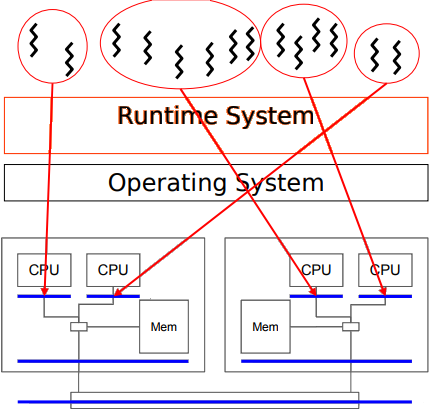
\includegraphics[scale=0.5]{bubbles001}
\centering
\caption{Principe de FORESTGOMP Framework}
\label{fig:mci7}
\end{figure}
%
\begin{center}%[htbp]
\begin{tabular}{l *{13}{l}} 		\hline
{TCH} & {IMP} 	& {SDP} 	&  {TSD} 	& {GRN} 	& {ToP} 	& {TYP} 	& {SPD}	& {ENT} 	& {ToS} \\     		\hline
C     	& OS		& PFL		&  - 		& PG		& EXE		& THD CLS	& OS 		& OS THD  & EXE  \\     		          \hline
\end{tabular}
 \captionof{table}{Caractéristiques de l'approche FORESTGOMP}% Add 'table' caption
\end{center}
%
\subsection{LAWS} %Task placement 	& Data distribution 	& Cilk tasks 	& Execution 	& x\\\lipsum 
%
\textbf{1- Auteurs}

Chen et al. \cite{Che38}

\textbf{2- Idée}

L'approche associe l'allocation et l'ordonnancement compatibles avec NUMA avec la programmation des tâches CILK. 
Elle cible les \textbf{algorithmes diviser pour régner} avec les caractéristiques suivantes: \\
a- les étapes récursives de l'algorithme sont représentées par un arbre de tâches dans lequel chaque nœud représente une étape.\\
b- les accès aux données ne se produisent que dans les tâches feuilles et le partage de données entre les tâches du même niveau dans l'arbre. 

LAWS a trois composants principaux: \\
i- un \textbf{allocateur de mémoire} compatible NUMA, \\
ii- un \textbf{packer DAG adaptatif}\\
iii- un \textbf{mécanisme de vol de travail} compatible avec NUMA et le cache. 

Son placement de données est effectué au cours de la première itération de l'algori-thme en affectant les ensembles de données des tâches crées de manière récursive de l'arbre de tâches aux nœuds NUMA.

\textbf{3- Expérimentation}

LAWS a été testé sur un système AMD Opteron 8380 à quatre nœuds exécutant un ensemble d'applications qui effectuent des \textbf{calculs de stencil} et des algorithmes pour l'\textbf{élimination gaussienne}. 
Chaque benchmark est disponible en deux versions. 
La première version a une exécution \textbf{DAG régulièrement structurée}, tandis que les calculs de la seconde version forment un \textbf{DAG de structure irrégulière}. 

\textbf{4- Evaluation}

La performance de LAWS a été comparée à CILK simple sans aucune modification et à un autre algorithme nommé CATS \cite{Che39}, qui n'adapte pas le placement après la première itération. 
L'amélioration de LAWS par rapport à CILK varie de 23:5\% à 54:2\%. 
LAWS surpasse systématiquement CATS, ce qui améliore les performances par rapport à CILK jusqu'à 19:6\%. 

\textbf{5- Commentaires}

LAWS montre que les informations implicites sur la structure des calculs ainsi que les structures de données impliquées dans les calculs peuvent être exploitées à la fois pour le placement de données et l'ordonnancement afin d'augmenter la localisation des accès mémoire automatiquement par le système d'exécution. 
%
\begin{center}%[htbp]
\begin{tabular}{l *{13}{l}} 		\hline
{TCH} & {IMP} 	& {SDP} 	&  {TSD} 	& {GRN} 	& {ToP} 	& {TYP} 	& {SPD}	& {ENT} 	& {ToS} \\     		\hline
C     	& RT		& DAG		&  ARY 	& BL		& EXE		& TSK		& DD 		& Cilk TSK 	& EXE  \\     		          \hline
\end{tabular}
 \captionof{table}{Caractéristiques de l'approche LAWS}% Add 'table' caption
\end{center}
%
Les tableaux 1.10 et 1.11 donnent un récapitulatif des caractéristiques principales pour toutes les approches présentées précédemment. 
%
\afterpage{
\clearpage% Flush earlier floats (otherwise order might not be correct)
\thispagestyle{empty}% empty page style (?)
\begin{landscape}
	\begin{center}%[htbp]

	\begin{tabular}{l *{13}{l}}
		\hline
	    	{Num} &     {Scheduling/Mapping Policy} &     {ONU} &     {OCH} &     {DPL} &     {SCH} &     {Impl layer} &     {DoRD} &  {Sup-DT} &     {Granularity} &     {ToD} &     {ADA} &    {Ref} \\
    		\hline
1		& Affinity on touch(OS)	& X 	& -		& X 	& - 	& LIB/OS		& PROGr 	& Any 			& PGs 			& EXE		& x 	& [61,50] \\
2         & CARREFOUR           		& X    	& -      & X     	& X     	& OS 			& PRFLg	& Any 			& PGs			& EXE		& x 	& [44] \\
3         & MAI                             & X    	& -      & X    	& -      	& LIB 			& PROGr 	& Arrays 		& BLs/PGs 		& EXE		& x 	& [77]\\
4         & MINAS + profiling         & X    	& X     	& X    	& (X)  	& PPg + LIB 	& PPr 		& Static Arrays & BLs/PGs 		& EXE		& x 	& [66,76] \\
5         & FBoPP 					& X    	& -      & X     	& -      	& LIB			& PRFLg 	& Any 			& PGs 			& EXE		& x 	& [62] \\
6         & SCHEDULE REUSE        & X    	& -      &(X)   	& X     	& CMPL+ RT	& PROGr 	& Arrays 		& ELTs			& EXE		& x 	& [68]\\
7         & Unstructured parallelism& - 		& X 	& - 	& X 	& RT			& - 		& - 			& - 			& EXE		& x 	& [86]\\
8       	& FORESTGOMP 			& X 	& X 	& X 	& X 	& RT			& PROGr 	& Not Specified& N/Specified	& EXE		& x 	& [29, 31]\\
9       	& LAWS 					& X 	& X 	& X 	& X 	& RT			& DAG 		& Arrays 		& BLs 			& EXE		& x 	& [38]\\
  		\hline
	\end{tabular}
	\label{table:TB_4_1_20}
	 \captionof{table}{Caractéristiques des approches et du placement de données associes}% Add 'table' caption

	\begin{tabular}{l *{8}{l}}
		\hline
		{Num} &     {Scheduling/Mapping Policy} &     {Type of placement} &     {Source for PLC decision} &     {Scheduling entity} &     {Time of decision} &     {Auto.dyn.adjustment}\\
		\hline
		1 		& Affinity on touch(OS)		& -    					& -      				& -     				& -      					& -\\
		2         & CARREFOUR                 	& Thread clustring   	& OS/PMU     		& OS threads     	& Execution     		& x\\
		3         & MAI                             	& Thread pinning    	& -      				& PThreads    		& Start of execution   	& -\\
		4         & MINAS + profiling              	& Co-scheduling    	& Data sharing     	& PThreads    		& Start of execution  	& -\\
		5         & Feedback-directed PLC 		& Thread pinning    	& -      				& PThreads     		& Start of execution    	& -\\
		6         & SCHEDULE REUSE            	& Loop scheduling   	& Data distribution & Loop iteration   	& Execution     		& -\\
		7         & Unstructured parallelism  	& Task placement 		& Data sharing 	& Tasks 			& Start of execution 	& x\\
		8        	& FORESTGOMP 			     & Thread placement	& Data distribution	& OpenMP threads	& Execution 			& x\\
		9         & LAWS 				     		& Task placement 		& Data distribution	& Cilk tasks 		& Execution 			& x\\
		\hline 
	\end{tabular}
	\label{table:TB_4_1_1}
	\captionof{table}{Caractéristiques de l'ordonnancement des approches vues}% Add 'table' caption
\end{center} 
\end{landscape}
\clearpage% Flush page
}
%===================================================================================
\newpage
\section{Stratégies d'équilibrage de charge dans NUMA}\label{straECNUMA}
%
L’algorithme d’ordonnancement dynamique doit être générique, évolutif et flexible sur la prise de décision. 
Cette flexibilité provient de la possibilité de choisir n’importe quelle tâche prête tout en conservant la borne sur le temps d’exécution.
Dans beaucoup d'algorithmes d'ordonnancement, l’objectif principal est de minimiser les temps d’inactivités et surtout cela lors de la communication. Pour aider à atteindre cet objectif, Les algorithmes de l'équilibrage de charge permettent de réduire cette inactivité en préservant une charge équitable entre les processeurs.

Chaque processeur maintient sa propre liste locale des tâches prêtes.
Cette commu-nication pourrait impliquer les transferts de données nécessaires pour compléter le travail, 
mais aussi les processeurs sont capables de communiquer pour échanger les tâches dans leurs files d'attente fonctionnelles. 
Le processus d'échange de tâches entre files d'attente est l'essence même de l'ordonnancement des algorithmes dynamiques. \cite{quint11}
Il existe deux grands paradigmes d'équilibrage de charge dynamique dans les plateformes parallèles NUMA inclus : \\
- Le partage de travail \cite{BL99}\\
- Le vol de travail \cite{BLU95}\\
%
\subsection{Partage du travail} 
%%Les processeurs partagent des tâches de leur liste prête aux listes prêtes d'autres processeurs. 
Dans la stratégie du partage de travail, chaque processeur a un ensemble de tâches à exécuter. 
Ce travail est enregistré dans la mémoire du processeur qui doit exécuter la tâche. 
Le risque est qu’un processeur ait plus de travail que les autres. 
Pour rééquilibrer la charge entre les processeurs, chaque processeur surveille sa quantité de travail . 
Si un processeur est surchargé, des tâches sont migrées vers les autres processeurs. 
Ainsi, les tâches sont échangées entre les processeurs pour équilibrer la charge.
Le choix de migration nécessite une méthode pour mesurer la quantité de travail totale et locale à un processeur, mais aussi le coût de la redistribution du travail. 
Au fur et à mesure de l’exécution, la quantité de travail diminue. 
Il est donc nécessaire de faire transiter des messages pour avoir les informations. 
Lorsque celles-ci sont connues, l’algorithme doit migrer les tâches afin d’obtenir un système dans lequel aucun processeur ne détectera de surcharge. \cite{quint11}

Pour les tâches homogènes et indépendantes, l’algorithme peut calculer la quantité de travail
sur toute la plate-forme et en local et il fonctionne bien dans ces conditions. 
En revanche, dans le cas général, cela implique des erreurs sur les temps d’exécution qui pourront être compensées par des migrations de tâches.
La prise en compte des relations de précédences et des coûts de communications entre les tâches compliquent sa tâche et demande d’importants changements dans l’algorithme. 
Dans ce cas, les migrations de tâches risquent d’être fréquentes pour compenser le manque d’informations.
Les performan-ces obtenues risquent d’être mauvaises. \cite{quint11}
%
\subsection{Vol de travail (Work stealing)}
%
Les processeurs tente de voler des tâches à partir de listes prêtes d'autres processeurs qui sont appelés \textbf{victimes (VICTIM)} lorsque sa propre file d'attente devient vide. 
Dans ce cas, ce processeur est appelé \textbf{voleur (THIEF)}, et la tâche volée migre vers la file d'attente de ce processeur en quittant celle du processeur volé \cite{SPO09}. 
Cet algorithme est implémenté dans certains langages comme Cilk \cite{BLU95}. 

L'objectif du vol de travail est de s’abstraire de toutes les données fournies par l’utilisateur tout en ordonnançant efficacement l’application sur un nombre de machines non défini. 
Ce mécanisme a été proposé initialement par Blumofe \cite{BLU95}.
Sa popularité provient de ses nombreux atouts, en voici  quelques un :\\
– algorithme distribué\\
– passage à l’échelle\\
– réactivité aux perturbations\\
– temps d’exécution et nombre de tâches transférées analysés théoriquement

%Une des principales propriétés du vol de travail est que l’algorithme est distribué.
Dans cet algorithme, les décisions sont généralement prises avec les informations locales à chaque processeur participant à l’exécution. 
Durant l’exécution, chaque processeur a une liste de tâches qui représente le travail à effectuer. 
Lors de l’exécution d’une tâche, le processeur exécute les instructions associées qui peuvent générer d’autres tâches. 
Ces tâches sont stockées pour la suite de l’exécution dans sa liste. 
L’ensemble des tâches et leurs données décrivent l’application qui est représentée par un DAG.
En fonction de la quantité de travail présente dans la liste, deux états sont distinguables pour les processeurs :
\\
- \textbf{Travailleur} ($NORMAL$) : un processeur qui exécute du travail (une tâche). Sa liste de tâches peut être vide ou non.\\
- \textbf{Victime} ($VICTIM$): un processeur qui exécute du travail (une tâche) et sa liste de tâches contient plus de tâches qu'un seuil fixé ($MAX\_TK$).\\
- \textbf{Voleur} ($THIEF$) : un processeur qui n’a plus de travail à exécuter. Sa liste de tâches est vide ou contient moins de tâches d'un seuil fixé ($MIN\_TK$).. 

Il tente de trouver du travail auprès des autres processeurs. 
Tous les processeurs évoluent entre ces trois états. 
Le passage de $THIEF$ à $NORMAL$ s’opère en demandant du travail aux autres processeurs. 
Si un processeur reçoit une demande de travail et s’il a des tâches dans sa pile, il envoie du travail au $THIEF$. 
Le passage de $NORMAL$ à $THIEF$ s’effectue en fonction des requêtes de vol et de l’exécution des tâches.
Dans ce mécanisme, l’ordre d’exécution des tâches est influencé par plusieurs décisions qui influencent énormément les performances du système : \\
1- la prochaine tâche à exécuter, \\
2- le processeur volé et la ou les tâches volées. \\
%
\subsubsection{Ordre d’exécution local}
%
L’ordre d’exécution est un des choix qui est le plus rarement modifié, car l’analyse théorique initialement réalisée par Blumofe et Leiserson \cite{BLU95},  montre que la décision de suivre le parcours initial du programme sans création de tâches (l’ordre séquentiel) est efficace. 
Le respect de l’ordre séquentiel permet de conserver les optimisations réalisées par le programmeur. 
De plus, ce choix permet de borner l’espace mémoire utilisé par chaque processeur. 
Cet espace mémoire est dans ce cas inférieur ou égal à l’espace mémoire utilisé par le programme séquentiel. 
Cet ordre d’exécution est équivalent à un parcours en profondeur du DAG de l’application. 
Au niveau de la liste, ce parcours peut être réalisé en sélectionnant la dernière tâche ajoutée ('Last In First Out (LIFO)').
%
\subsubsection{Requête de vol}
%
Lorsqu’un processeur devient $THIEF$, il choisit le processeur $VICTIM$ duquel il va prendre une partie du travail. 
Il existe un grand nombre de stratégies différentes. 
Une des stratégies pour le choix est simplement de réaliser un tirage aléatoire uniforme parmi les processeurs participant à l’exécution. 
Cette stratégie reste la plus simple, ne nécessitant aucune information avec un nombre de requêtes de vol borné.
Les analyses théoriques montrent qu’avec une telle sélection de la victime, la probabilité de sélectionner un processeur ayant une
quantité importante de travail est grande même avec un nombre limité de vols \cite{BLU95}.

Une autre stratégie qui choisit le processeur ayant la tâche la moins profonde dans sa pile.  
Cette solution minimise le temps d’exécution, mais elle nécessite de conserver une information du processeur possédant cette tâche sur toute la plateforme.
Pour prendre en compte l’influence des accès mémoires sur des plates-formes hiérarchiques ou non, des travaux ont montré qu’il est intéressant d’orienter les vols vers des tâches ayant des données qui pourront être accédées rapidement par $THIEF$. \cite{quint11}
%
\subsubsection{Réponse de vol}
%
Sur réception d’une requête de vol, un processeur doit sélectionner le travail à fournir.
L’algorithme réalisant la sélection du travail à transférer vers $THIEF$ s’exécute en concurrence du travail effectué par le processeur $VICTIM$. 
Classiquement dans le vol de travail, la dernière tâche ajoutée à la pile est la tâche sélectionnée pour être exécutée.
Ainsi, les processeurs accèdent à leur pile par le bas (ordre 'LIFO'). 
Pour ne pas perturber le travail de la victime, les tâches volées sont choisies prioritairement en haut de la pile (ordre 'FIFO'). 
Les conflits d’accès risquent d’apparaître uniquement quand le nombre de tâches est faible. 
Il reste à définir le nombre de tâches prises dans la pile. 
Lors d’un vol, l’objectif est d’équilibrer le travail entre les deux processeurs ($VICTIM$ et $THIEF$). 
Puisque $THIEF$ n’a pas assez de travail, la quantité de travail prise doit être proche de la moitié de celle présente sur la victime. 
%------------------------------------------------------------------------------------------
\newpage
\section{Conclusion}\label{concEdA}
%
Dans ce chapitre, nous avons exposé les différentes approches concernant l'ordon-nancement et le placement des tâches avec les données dans le contexte NUMA. 
Au début, nous avons caractérisé de façon générique les approches qui tentent d'assurer un de ces rôles de point de vue prise décision. Ces approches sont basées sur  certaines caractéristiques des architectures cibles et certaines informations à exploiter lors de son fonctionnement. En se basant sur ces caractéristiques, nous pouvons regrouper les approches en trois classes. la première qui focalise sur l'ordonnancement seulement, la deuxième sur le placement et la troisième combine les deux aspects.

Par la suite, nous avons présenté l'idée derrière chaque approche ainsi que son implémen-tation et son évaluation. A la fin de chaque section, nous avons commenté les avantages et les limites de l’approche étudiée. Cette démarche nous permet de comparer l'impact de l'intégration  de chaque approche sur les performances des systèmes NUMA. 

Comme l'équilibrage de charge est important pour préserver les performances, la dernière section a détaillé les stratégies utilisées pour cette fin en particulier celle du vol de travail qui nous intéresse par la suite.

Le chapitre suivant est dédié à présenter notre approche dont le principe est d'exploiter l'horizon d'exécution pour guider les processus d'ordonnancement et exposer une variante de vol de travail basé sur la distance NUMA.
	\chapter{Horizon d'exécution étendu et Vol de travail adaptatif}\label{chapter:HX}
%
Dans ce chapitre nous allons présenter les heuristiques proposées pour ordonnancer et placer les threads d'une application décrite par un DAG sur la plateforme NUMA multicoeur. L'\textbf{horizon d'exécution étendu X-VHFU (eXtended Visible, in Horizon, Far and Unseen)} et le \textbf{vol de travail adaptatif basé sur la distance (distance based Work Stealing)} sont les deux idées de base proposées dans cette thèse. 

La première section \ref{schSOP} va exposer l'étude de la combinaison des politiques d'ordo-nnancement et les placements existants appliqués sur des applications constituées d'une séquence de tâches indépendantes. 
Ensuite, nous présentons nos approches dans la deuxième section \ref{OPGT}.
Dans la troisième section \ref{EC}, l'algorithme de l'équilibrage de charge est exposé dont l'heuristique de base est le vol de travail basé sur la distance.
Enfin, la section \ref{conc} conclue le chapitre.
%au premier temps, nous allons les appliquer sur une classe particulière de DAG qui représente les applications parallèles décrites par le modèle de programmation parallèle  fork-join. Ensuite, nous donnons la version généralisée.
%====================================================================================
\section{Schémas des stratégies d'ordonnancement et placement }\label{schSOP}
%
Les algorithmes O/M suivent le même motif structurel, ils diffèrent seulement par la stratégie de la sélection de l'entité courante à être servie. Les schémas algorithmiques suivants explicitent cette idée :

Le schéma pour l'\textbf{ordonnancement des tâches} : il fonctionne selon la stratégie client / serveur en attendant la soumission des tâches à exécuter, il attend la disponibilité d'une ressource d'exécution et puis il choisit la tâche qui optimise une heuristique donnée, enfin il programme l'exécution de celle-ci sur la ressource libérée. Ce schéma est de nature distribuée événementielle selon le motif \textbf{observateur/observable}. L'algorithme \textbf{scheduleTasks} associé avec les évènements \textbf{Event\_OnTaskSubmission} et  \textbf{Event\_-OnTaskExecutionEnd} illustre le principe de ce dernier.

Le schéma pour le \textbf{placement des données} des tâches : il fonctionne selon la stratégie client / serveur en attendant les requêtes des tâches pour charger des données en mémoire ou vers le processeur (deux types de requêtes allocation et libération de la mémoire lecture/écriture des pages/blocs mémoire), il attend la disponibilité d'une ressource de stockage (mémoire) et puis il choisit la requête qui optimise une heuristique donnée, enfin il alloue un espace mémoire dans la mémoire cible pour les données choisies . Ce schéma est aussi de nature distribué évènementiel selon le motif \textbf{observateur/observable}. L'algorithme \textbf{mapTaskData} associé avec les évènements \textbf{Event\_OnTaskAllocateMe-mory}, \textbf{Event\_OnTaskFreeMemory}, \textbf{Event\_OnTaskExecutionStart} et \textbf{Event\_-OnTaskExecutionEnd} illustre le principe de ce dernier.
%-----------------------------------
%\IncMargin{1em}
\begin{algorithm}
\DontPrintSemicolon
\SetNoFillComment % <---------------------------
\SetKwInOut{Input}{input}\SetKwInOut{Output}{output}

%\& $A^* \neq \emptyset$
\Input{A DAG G=(V,E) and a toplogy graph TG=(N,P,L)}
\Output{A schedule of G on TG}

\BlankLine 
\textbf{Function } initialize()\\ 
\Begin{
     \tcc{Q : ready tasks queue , A : available cpus}
	$Q^* \longleftarrow \{T_0\}$ \\
	$A^* \longleftarrow P^*$ \\
	processNotyetScheduledTasks()
}

\BlankLine 

\textbf{Function } processNotyetScheduledTasks()\\ 
\Begin{
	\While { $Q^* \neq \emptyset$} {  
		//ready tasks not executed yet\\
	     \tcc{$T_s$ : selected task to be scheduled now}
		$T_s = $ argMax$_{t \in Q^*}$  TaskSelectionHeuristic($t$)\\
		\If { $T_s \neq \textbf{null}$} { 
			$P_s = $argMax$_{p \in \mathbb{A^*}}$  ProcesseurAllocationHeuristic($p$, $T_s$)\\
			\If { $P_s \neq \textbf{null}$  } {
	     		\tcc{$P_s$ : processor to be allocated now} %				$Q^* = Q^* - \{T_s\}$\\%	$A^* =A^* - \{P_s\}$ 
				Trigger OnTaskExecutionStart($T_s$, $P_s$)\\
				scheduleOn($T_s$, $P_s$).
			}
		}
	}
}

\BlankLine 

\tcc{On task start event}
\textbf{Event }  OnTaskExecutionStart($T$, $P$) \\
\Begin{
	$Q^* = Q^* - \{T_s\}$\\
	$A^* =A^* - \{P\}$ 
}

\tcc{On task end event}
\textbf{Event }  OnTaskExecutionEnd($T$) \\
\Begin{
	$R^*$ = getReadyNeighboursAfterEndOf($T$)\\
	$P$ = getAllocatedProcessorTo($T$)\\
	$Q^* = Q^* \cup R^*$ \\
	$A^* = A^* \cup \{P\}$\\
	processNotyetScheduledTasks()\\
}

\caption{Algorithme générique d'ordonnancement des taches}
\end{algorithm}
%\DecMargin{1em}
%----------------------------------

%-----------------------------------
%\IncMargin{1em}
\begin{algorithm}
\DontPrintSemicolon
\SetNoFillComment % <---------------------------
\SetKwInOut{Input}{input}\SetKwInOut{Output}{output}

%\& $M^* \neq \emptyset$
\Input{A DAG G=(V*,E*) and a toplogy graph TG=(N*[P*,M],L*)}
\Output{A schedule of G on TG}

\BlankLine 

\textbf{Function } initialize()\\ 
\Begin{
     \tcc{$D^*$ : tasks load request data , $M^*$ : available memory pages}
	$D^* \longleftarrow \{T_0.data\}$ \\
	$M^* = getFreeMemoryPages()$ \\
	processnotyetMappedTasksData()
}

\BlankLine 

\textbf{Function } processnotyetMappedTasksData()\\ 
\Begin{
	\While { $D^* \neq \emptyset$} {
	     \tcc{$D^*$ : selected tasks data to be mapped now}
		$S^* = $argMax$_{d \in S^*}$  TaskDataSelectionHeuristic($d$)\\
		\If { $S^* \neq \emptyset$  } {
		     \tcc{$P^*$ : memory pages to be allocated now}
			$D^* = D^* - \{S^*\}$\\
			$P^*_s = $argMax$_{m \in \mathbb{M^*}}$  MemoryMappingHeuristic($m$ , $S^*$)\\
			$M^* =M^* - P^*_s$
		}
	}
}

\BlankLine 

\tcc{On task data load request event}
\textbf{Event }  OnTaskDataLoadRequest($T$,$L^*$) \\
\Begin{
	$D^* = D^* \cup \{L^*\}$\\
	Trigger OnTaskAllocateMemory()
}

\tcc{On task allocate memory event}
\textbf{Event }  OnTaskAllocateMemory() \\
\Begin{
	processnotyetMappedTasksData()
}

\tcc{On task free memory event}
\textbf{Event }  OnTaskFreeMemory($P^*$) \\
\Begin{
	$M^* = M^* \cup \{P^*\}$\\
	processnotyetMappedTasksData()
}

\caption{Algorithme générique de placement des données des taches}
\end{algorithm}
%\DecMargin{1em}
%====================================================================================
\newpage
\section{Ordonnancement et placement des tâches  indépendantes}\label{OPTI}
%
Dans cette section nous allons présenter le cas ou les tâches de l'application sont indépendantes et partagent des données. Dans ce contexte, nous essayons de voir l'impact de la combinaison des différentes politiques d'ordonnancement et de placement sur les performances des applications parallèles. Cela va nous aider à évaluer la  corrélation entre l'ordonnancement et le placement dans le contexte NUMA sans avoir une structure particulière de l'application exécutée. Cette première stratégie nous permet de voir les facteurs influents sur le calcul (exécution) indépendamment de la communication et l'échange des données et d'inspecter le comportement de la plateforme et sa réaction lorsque nous exécutons la même suite de tâches parallèles indépendantes mais en changeant la paire (politique ordonnancement / politique placement) et l'influence de ce fait sur les performances du support exécutif et en particulier le temps total d'exécution, le facteur NUMA et l'équilibrage de charge.
%
\subsection{Combinaison des politiques d'ordonnancement/placement classiques}
Par la suite, nous utilisons certaines politiques implémentées sur les plateformes actuelles pour l'ordonnancement on a :
%
\subsection{Politiques d’ordonnancement classique}
%
\subsubsection{Politique à tour de rôle (Round Robin RRS)} 
%
C'est la politique la plus simple à implémenter elle consiste à allouer les nœuds de calcul aux tâches arrivantes à tour de rôle. Si \textbf{m} est le nombre de nœuds disponibles pour exécution des tâches, et \textbf{(k+1)} est l'ordre d'arrivée de la tâche $T_{k+1}$ (k est le nombre des tâches déjà ordonnancées, cette tâche sera l'entête de la queue \textbf{Q} utilisée pour mettre en file d'attente les tâches reçues. L'heuristique de la sélection des tâches appelle \textbf{Q.pop()} alors cette tâche sera affectée au nœud \textbf{k=n mod m} si ce dernier est libre.
\[
N^*[(k+1) mod |N^*|]
\]
%
\subsubsection{Politique le moins utilisé (LessUsed)}
%
Elle consiste à affecter les tâches arrivantes au nœud le moins utilisé parmi les ressources libres.
\[
		\text{argMin}_{a \in A^*} \text{getProcessorNumberOfUses}(a)
\]
%
\subsubsection{Politique le moins chargé (Less Loaded LLS)}
%
Cette stratégie consiste à surveiller la charge courante de la plateforme en mainte-nant une structure de donnée qui représente sa charge et d'affecter la tâche courante au nœud le moins chargé. L'heuristique de l'allocation détermine argMin des processeurs en fonction de leurs charges obtenues par une fonction getProcessorLoad(p) : 
\[
		\text{argMin}_{a \in A^*} \text{getProcessorsLoad}(a)
\]
%
\subsection{Politiques de placement classique}
%
Nous utilisons des politiques similaires implémentées sur les plateformes actuelles pour le placement et ainsi que d'autre spécifiques au contexte NUMA, on a  :
%
\subsubsection{Placement à tour de rôle (Round Robin RRM)}
%
C'est la politique la plus simple à implémenter elle consiste à allouer les mémoires des nœuds aux tâches à tour de rôle afin de stocker leurs données.
\[
M^*[(k+1) mod |M^*|]
\]
%
\subsubsection{Politique le moins utilisé (LessUsed)}
%
Elle consiste à affecter les tâches arrivantes au nœud le moins utilisé parmi les ressources libres.
\[
		\text{argMin}_{m \in M^*} \text{getMemoryNumberOfUses}(m)
\]
%
\subsubsection{Placement First Touch}
%
Les données d'une tâche seront stockées sur la mémoire du nœud responsable de l'exécution de la tâche associée. Lorsqu’une tâche demande le chargement d'une donnée, le mapper vérifie si elle est déjà chargée dans la mémoire d'un nœud sinon elle sera chargée dans la mémoire du nœud sur lequel la tâche est ordonnancée.%\begin{verbatim}  This is a verbatim block.\end{verbatim}
\[
{\footnotesize
\text{if (T}_i\text{.Load(Data}_j\text{) and Data}_j\text{.State == 'UNLOAD') M[getAllocatedNodeFor(T}_i\text{)].Load(Data}_j\text{)}
}
\]
%
\subsubsection{Placement Next Touch}
%
Les données d'une tâche seront stockées sur la mémoire du nœud responsable de l'exécution de la tâche associée. Lorsqu’une tâche demande le chargement d'une donnée, le mapper verifie si elle est déjà chargée dans la mémoire d'un nœud, alors il va faire migrer cette tâche sinon elle sera chargé dans sa mémoire.%
\[
{\footnotesize
\text{if (T}_i\text{.Load(Data}_j\text{) and Data}_j\text{.State == 'LOAD') M[getAllocatedNodeFor(T}_i\text{)].Migrate(Data}_j\text{)}
}
\]

Les politiques combinées sont round robin RRS, moins utilisé LUS et less loaded LLS pour la stratégie de l'ordonnancement et round robin RRM, moins utilisé LUM, first touch FTM et next-touch NTM pour les stratégies de placement. nous obtenons douze combinaisons.
%====================================================================================
\newpage
\section{Ordonnancement et placement d'un graphe de tâches}\label{OPGT}
%
Dans cette section, nous présentons les idées derrières les heuristiques proposées  ainsi que les algorithmes associés.
%
\subsection{Heuristique Horizon d'exécution Etendu X-VHFU}
%
L'heuristique proposée est constituée de quatre phases. 
Au début de l'exécution, on extrait la \textbf{topologie du DAG} ainsi que les \textbf{informations de communication} (les références et la taille des données utilisées et partagées par les tâches). Cette phase préliminaire est basée sur les annotations faites par le programmeur dans le code source et qui seront convertit à une information utilisée par le support d'exécution. En se basant sur cette topologie on \textbf{partitionne le DAG en sous DAGs} de tailles presque similaire initialement,  
ensuite elle les \textbf{attache aux nœuds} de la plateforme (Fixer les préférences des tâches). 
Lors de l'ordonnancement d'une tâche, en fonction de son horizon d'exécution courant, elle est sélectionnée pour être exécutée soit sur le nœud du sous DAG à lequel cette tâche appartienne ou un autre selon son état courant. Si un autre nœud est choisi alors la configuration des sous DAGs est actualisée en recalculant les nouveaux sous DAG et en appliquant globalement une stratégie dite \textbf{horizon d'exécution X-VHFU} sur le DAG apres ce changement. 
Enfin, elle \textbf{équilibre la charge} en utilisant une stratégie de vol des travaux adapté et basé sur la distance au contexte NUMA.
%
\subsubsection{Partitionner le DAG}
%
Dans cette phase, le DAG $G(V^*,E^*)$ donné est partitionné en $K$ sous DAGs  $(G_i)_{i:1..K}$ en utilisant un algorithme du partitionement des graphes adapté à ce contexte. Dans ce cas , notre graphe sera pondéré avec le volume des donnés échangés entre les tâches (qui peut être obtenu au début l'analyse de notre DAG cible) et non par le temps de la communication entre les tâches (inconnu dans ce contexte). 
Le résultat de cette phase est une partition $G$.   %trouvés dans littérature [@1,@2,@3] 
%
$$
\Phi(G) = (\{ G_1, G_2, \cdots , G_K\}, Mx_{K \times K}) 
$$
$$
G_i = (V^*_i, E^*_i) \text{ vérifiant la relation } \bigcup_{1 \le i \le K} V^*_i = V^* \&  V^*_i \cap V^*_j = \emptyset \text{ , } \forall i \neq j
$$
%
Où $Mx_{K \times K}$ est la matrice de flux inter sous-graphes (volume de données échanger entre les tâches des sous graphes connectés) et $G_i$ le sous graphe numéro $i$. 
Dans un premier temps, notre algorithme doit déterminer les différents niveaux des sommets sur le DAG donné, ensuite il parcourt chaque niveau en essayant d'affecter le sommet courant à un sous graphe qui minimise le flux des données échangées avec le reste des sous graphes déjà calculer.
%----------------------------------%\IncMargin{1em}
\begin{algorithm}
\DontPrintSemicolon
\SetNoFillComment % <---------------------------
\SetKwInOut{Input}{input}\SetKwInOut{Output}{output}

%
\Input{un graphe de tâche DAG G=(V*,E*), La matrice du flux données échangées entre les sommets Md, le nombre des partitions K}
\Output{une partition PAR P = [G*, Mx*], G* l'ensemble des sous DAGs et Mx* : matrice du flux entre les sous DAGs}

\BlankLine 
%\textbf{Function } initialize()\\ 
\Begin{
	L =  getGraphLevels(G)  //Levels\\
	\ForEach{$l \in L$}{
		\ForEach{$v \in l$}{
	$\text{                                                                  }$           j = argMin$_{1 \le i \le K }$ computeEgdeCutWeight(v,G,Md,G*[i],Mx)\\
	$\text{                                                                  }$           G*[j].addVertex(v)\\
	$\text{                                                                  }$           updateEgdeCutWeightMatrix(v,G,Md,G*[j],G,Mx)\\
		}
	}
}

\textbf{Function } getGraphLevels(G(V*,E*))\\ 
\Begin{
	$U = V*$
	$i = 0$\\
	$Levels[i] = $ getVertexWithoutPredecessorsIn(G,U)\\
	\While { $U \neq \emptyset$} {
		$U = U - Levels[i]$\\
		$i++$\\
		$Levels[i] = $ getVertexWithoutPredecessorsIn(G,U)\\
	}
	Return $Levels$
}
\caption{Partitionnement d'un DAG en sous DAGs}
\end{algorithm}              %\DecMargin{1em}
%----------------------------------
Cet algorithme utilise les fonctions helper suivantes :

- \textbf{getGraphLevels(G)} : cette fonction détermine l'ensemble des niveaux des sommets de notre DAG donnée. Comme vu dans le chapitre 2 graphe de tâches, un niveau de rang $l$ dans un DAG est un ensemble de sommets dont les sommets parents sont tous dans le niveau de rang strictement inferieur ou égale à $l-1$ et au moins un sommet parent dans le niveau $l-1$.  le niveau du rang 1 est constitué de l'ensemble des sommets qui n'ont pas de prédécesseurs. La figure \ref{fig:FG_4_1} illustre un DAG avec plusieurs niveaux. 

- \textbf{getVertexWithoutPredecessorsIn(U)} : Cette fonction détermine l'ensemble des sommets qui n'ont pas des sommets prédécesseurs dans l'ensemble $U$. Elle permet de trouver les sommets du niveau courant.

- \textbf{computeEgdeCutWeight(v,G,Md,G*[i],G,Mx)} : cette fonction permet de calculer le flux des données échangés résultant de considérer le sommet $v$ dans le sous graphe $G^*[i]$ en utilisant la matrice des flux trouvée $Mx$. 

- \textbf{updateEgdeCutWeightMatrix(v,G,Md,G*[j],G,Mx)} : cette fonction met à jour la matrice des flux après avoir ajouté $v$ au sous graphe $G^*[j]$.

La figure \ref{fig:FG_4_2} donne un exemple de l'application du processus du partitionnement du DAG donné dans la figure \ref{fig:FG_4_1}. Les sous DAGs résultants sont montrés avec différentes couleurs. 
%
\begin{figure}
\includegraphics[scale=0.6]{dag050}
\centering
\caption{DAG avec plusieurs niveaux}
\label{fig:FG_4_1}
\end{figure}
%
\begin{figure}
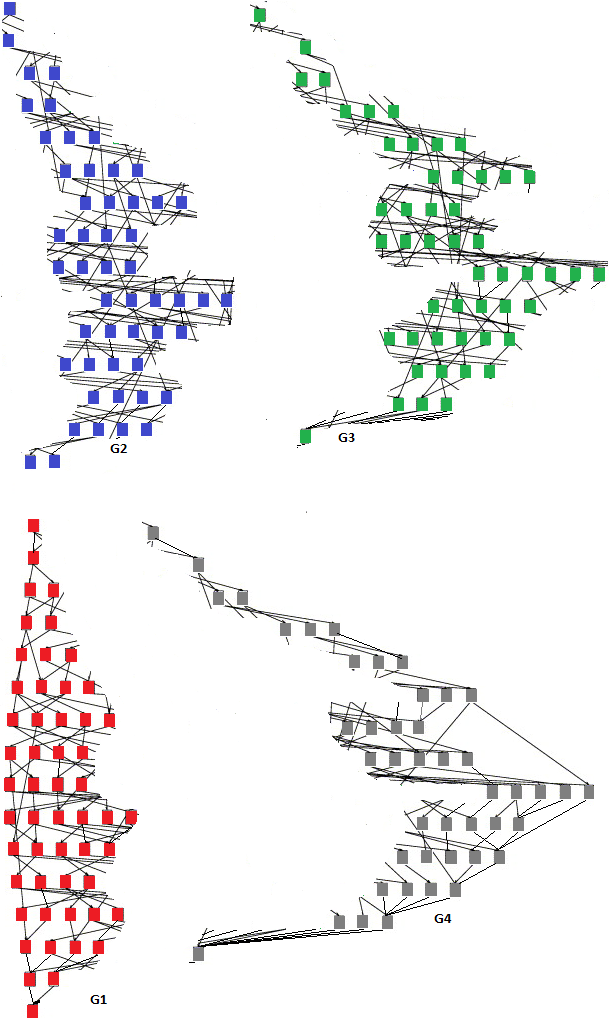
\includegraphics[scale=0.5]{dag053}
\centering
\caption{Resultat de la partition d'un DAG}
\label{fig:FG_4_2}
\end{figure}
%
\subsubsection{Fixer les préférences de tâches en fonction des sous DAGs}
%
Cette deuxième phase consiste à attacher (bind) chaque sous-DAG $G_i$ à un nœud particulier $N_j$ qui sera le nœud espéré d'exécution  des tâches de $G_i$. Cette préférence peut être changée en fonction de l'état actuel du processus généré par l'exécution du DAG $G$.
Cette affectation peut être considérée comme un ordonnancement initial qui  sera actualisé au fur et à mesure qu'on avance dans le processus.
%
$$
\Phi(\{ G_1, G_2, \cdots , G_n\}*, \{N_j\}) = \{(G_{i_1},N_{j_1}), (G_{i_1},N_{j_1}), \cdots, (G_{i_n},N_{j_n}) \}
$$
%----------------------------------%\IncMargin{1em}
\begin{algorithm}
\DontPrintSemicolon
\SetNoFillComment % <---------------------------
\SetKwInOut{Input}{input}\SetKwInOut{Output}{output}

%
\Input{une partition PAR P = [G*, Mx*], matrice des distances NUMA Dx}
\Output{une liste de paires [(G$_i$, N$_j$) i $\in$ I, j $\in$ J] }

\BlankLine 
%\textbf{Function } initialize()\\ 
\Begin{
	Nd* = getAllNode(Dx)\\
	L = $\varnothing$\\
	\ForEach{G$_i$ $\in$ G*}{
%	$\textbf{foreach}$ G$_i$ $\in$ G*\{\\
	$\text{                                                                  }$           N$_j$ = getPreferenceNode(Nd*, G*, G$_i$)\\
	$\text{                                                                  }$           Nd* = Nd* /{N$_i$}\\
	$\text{                                                                  }$           L.addItem((G$_i$,N$_j$))\\
%	$\textbf{endfor}$\\
	}
}

\caption{Préférence d'exécution des sous DAGs}
\end{algorithm}              %\DecMargin{1em}
%----------------------------------
La fonction \textbf{getPreferenceNode(Nd*, G*, G$_i$)} permet de faire une correspondance (bijection, matching) entre les nœuds de la plateforme et les sous DAGs trouvés. Comme le nombre de nœuds $K$ est égal au nombre des sous DAGs alors ce matching revient à trouver une permutation des nœuds dont le nombre est $K!$ qui préserve la relation du voisinage existante entre les sous DAGs en affectant deux sous DAGs voisins sur des nœuds voisin. On peut choisir une métrique qui quantifie une permutation donnée (distance euclidienne ou autre) et ensuite prend le minimum. 
%
\subsubsection{Appliquer la stratégie horizon d'exécution étendu X-VHFU}
%
Lors de l'ordonnancement, la prise de décision de quelle tâche à sélectionner et sur quel nœud doit être exécutée est faite en fonction de l'état actuel du processus correspondant au DAG exécuté. 
%
Apres avoir décidé la tâche à exécuter $T_c$ et le nœud exécutant alors on maintient un partitionnement basé sur la visibilité des tâches au support exécutif. 
Traditionnellement, à un moment donné pendant l'exécution de l'application parallèle décrite par un DAG, l'ensemble des tâches $\mathbb{T}$ est partitionné en quatre catégories :\\
1- Tâches complètes ($C$),  $ T_C$ : Les tâches finies (completed tasks)\\
2- Tâches en exécution $X$, $ T_X$ :  Les tâches en exécution (running tasks)\\
3- Tâches prêtes $R$ (ready task) \\
4- Tâches non prêtes $Q$ (not ready yet task).
%
$$ 
T_R = \{ T \in \mathbb{T} |\forall \text{Parent}(T) \in T_C \}
$$
$$
T_Q = \{ T \in \mathbb{T} | \exists \text{Parent}(T) \notin T_C \}
$$
$$
\mathbb{T} = T_C \cup T_X \cup T_R \cup T_Q
$$
%
Afin de contrôler mieux cette exécution, on partitionne davantage la dernière catégorie $Q$ pour prévoir les tâches visibles à l'instant courant en se basant sur l'information disponible au support exécutif à ce moment (les tâches complètes $C$, les tâche en exécution $X$, tâches prêtes $R$). Cette vision est une extension de la visibilité immédiate à un niveau avancé qui permet d'aller au delà des tâches prêtes $R$. Les nouvelles catégories sont :
%
$$
T_Q = T_V \cup T_H \cup T_F \cup T_U
$$
%
\textbf{Les tâches visibles  $V$ (visible task)}:\\
Les tâches à l'horizon 0, ce sont les tâches qui ont au moins une tâche prédécesseur en exécution et tous autre prédécesseurs sont des tâches  complètes ou en exécution. Apres la terminaison des prédécesseurs qui sont en exécution, Cette tâche change d'état et devient prête. Cette classe de tâche a une forte probabilité d'être exécuté prochainement. 
%
$$
T_V  = \{ T \in \mathbb{T} | \forall \text{Parent}(T) \in T_C \cup T_X \text{ et } \exists \text{Parent}(T) \in T_X \}
$$
% 
\textbf{Les tâches dans l'horizon $H$ (horizon task)} : \\
Les tâches à l'horizon 1, ce sont les tâches qui ont au moins une tâche prédécesseur prête et tous autre prédécesseurs sont des tâches  complètes, en exécution ou prête. On attend que leurs tâches prédécesseurs se terminent avant qu'elles deviennent prêtes. Cette classe de tâche a une probabilité moyenne d'être exécuté prochainement. 
%
$$
T_H  = \{ T \in \mathbb{T} | \forall \text{Parent}(T) \in T_C \cup T_X  \cup T_R  \text{ et } \exists \text{Parent}(T) \in T_R \}
$$
%
\textbf{Les tâches au-delà de l'horizon $F$ (beyond the horizon task)} :\\  %$T_U$ : Les tâches non visibles   \\
Les tâches au-delà de l'horizon non visibles immédiatement qui ont au moins une tâche prédécesseur visible et tous autres prédécesseurs sont des tâches  complètes, en exécution ou visibles. 
%
$$
T_F  = \{ T \in \mathbb{T} | \exists \text{Parent}(T) \notin T_C \cup T_X  \cup T_V  \text{ et } \exists \text{Parent}(T) \in T_V \}\}
$$
%
\textbf{Les tâches non visible $U$ (unseen task)} :\\  %$T_U$ : Les tâches non visibles   \\
Les tâches non visibles sont les tâches qui ont au moins une tâche prédécesseur qui est ni complète, ni en exécutons, ni prête et ni visible. Elles peuvent être loin du niveau actuel de l'exécution. Nous n'avons aucune information qui permet d'évaluer à quel point cette tâche est loin d'être exécutée prochainement. 
%
$$
T_U  = \{ T \in \mathbb{T} | \exists \text{Parent}(T) \notin T_C \cup T_X  \cup T_R  \cup T_V \}
$$
%
Ce partitionnement va nous permettre d'anticiper certaines décisions et de se projeter dans le future prochain de l'exécution de l'application courante. Un nouveau critère de sélection de la tâche courante vient d'être intégré dans le processus de la décision. La prise de décision $D_c$ que l'ordonnanceur doit assurer à chaque libération d'une ressource d'exécution est maintenant une combinaison de trois facteur :
%décision = \Phi(préférence , affinité, horizon) \\
$$
D_c = \Phi(P_f , A_f, H_z) 
$$
%
\textbf{Préférence} $P_f$ : le nœud à lequel le sous DAG qui contient la tâche concernée est attaché.\\
\textbf{Affinité} $A_f$ : le nœud sur lequel une bonne partie des données utilisé par la tâche concernée y résident.\\
\textbf{Horizon} $H_z$ : A quel point si on sélectionne la tâche concernée, on va avancer dans l'horizon d'exécution (on va voir plus de tâches et on s'approche plus de la fin). 

Donc, on partitionne l'ensemble des tâches en fonction de l'horizon d'exécution actuelle (est ce que elle est déjà exécutée ou en court d'exécution, prête, dans l'horizon ou loin d'être exécutés dans le future prochain).
%
\begin{figure}
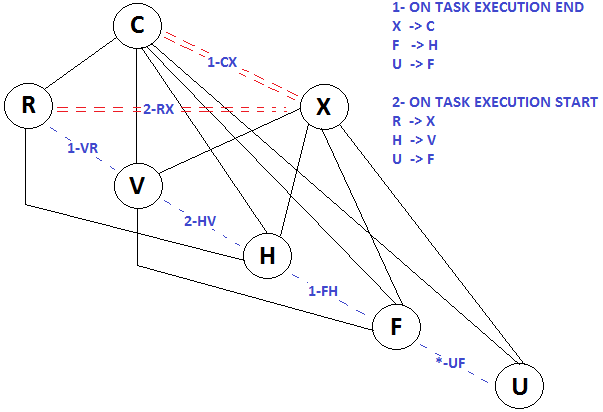
\includegraphics[scale=0.75]{vhfu001}
\centering
\caption{Graphe de transformation des niveaux de visibilité}
\label{fig:FG_4_10}
\end{figure}
%----------------------------------%\IncMargin{1em}
\begin{algorithm}
\DontPrintSemicolon
\SetNoFillComment % <---------------------------
\SetKwInOut{Input}{input}\SetKwInOut{Output}{output}

%
\Input{la tâche récemment terminée ou commencée $T_f$ }
\Output{L'horizon d'exécution courant VHFU}

\BlankLine 
\tcc{On task end event}
\textbf{Event }  OnTaskExecutionEnd($T_e$) \\
\Begin{
	$T_X = T_X - T_e$\\	
	$T_C = T_C \cup {T_e}$\\

     \tcc{update the ready tasks}
	$T_R = T_R \cup $ updateSpecifiedHorizon($T_V$, $T_C$)\\

     \tcc{update the visible tasks}
	$T_H = T_H \cup $  updateSpecifiedHorizon($T_F$, $T_R$)\\

     \tcc{update the visible tasks}
	$T_F = T_F \cup $ updateSpecifiedHorizon($T_U$, $T_V$)\\
}

\BlankLine 
\tcc{On task start event}
\textbf{Event }  OnTaskExecutionStart($T_s$) \\
\Begin{
	$T_R = T_R - T_s$\\	
	$T_X = T_X \cup {T_s}$\\

     \tcc{update the ready tasks}
	$T_V = T_V \cup $ updateSpecifiedHorizon($T_H$, $T_X$)\\

     \tcc{update the visible tasks}
	$T_F = T_F \cup $ updateSpecifiedHorizon($T_U$, $T_V$)\\
}

\tcc{update the specified horizon}
\textbf{Function} updateSpecifiedHorizon($T_A$, $T_B$ )\\
\Begin{
	$V^* = \varnothing$\\
	\ForEach{A$_i$ $\in$ $T_A$}{   %	$\textbf{foreach}$ Q$_i$ $\in$ $Q^*$\\
		\If { $A_i$.getParents() $\subset  T_C \cup T_X  \cup T_B$ and $A_i$.getParents() $\cap T_B \neq \varnothing$  } {
			$V^* = V^* \cup \{ A_i \}$\\
		}
	}
	Return $V^*$
}

\caption{Algorithme Horizon d'exécution étendu XH-VHFU}
\end{algorithm}              %\DecMargin{1em}
%----------------------------------
\begin{figure}
\includegraphics[scale=1]{dag054}
\centering
\caption{DAG avec plusieurs niveaux}
\label{fig:FG_4_1}
\end{figure}

\begin{figure}  %[h]
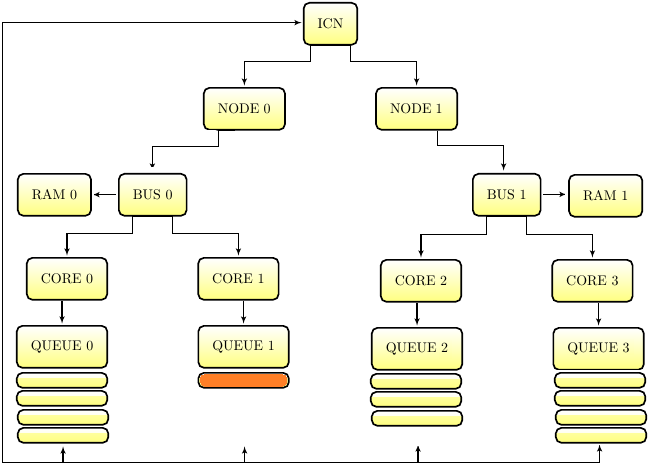
\includegraphics[scale=0.5]{adag003}
\centering
\caption{Plateforme NUMA et stratégie de vol de travail}
\label{fig:hm001}
\end{figure}
%
Le principe de la sélection de la tâche prête à exécuter $T_s$ à un moment donné par l'ordonnanceur est basé sur l'idée de choisir celle qui va élargir l'horizon d'exécution après le changement de son état vers l'exécution pour une meilleure visibilité afin d'avoir plus d'informations qui aident à mieux ordonnancer les tâches suivantes et mieux placer les données associées. Pour déterminer cette tâche $T_s$, l'algorithme parcourt l'ensemble des tâches prêtes $T_R$ et pour chacune d'elle $T_r$ nous allons évaluer la mise à jours de l'horizon de l'exécution $\Delta H(T_r)$ causée par son changement d'état. Cette quantification est une combinaison pondérée du changement de chaque classe de visibilité. De façon intuitive, nous cherchons combien de tâche devient prête $\Delta V(T_r)$, visible $\Delta H(T_r)$, dans horizon $\Delta F(T_r)$ ou au-delà de l'horizon $\Delta U(T_r)$ après avoir choisi d'exécuter la tâche $T_r$. Les classes de visibilité n'ont pas le même degré d'influence ou d'importance sur le processus d'ordonnancement ou placement. La classe visible renseigne ce processus mieux que celle de l'horizon et cette dernière apporte plus d'informations que celle de l'au-delà de l'horizon et en dernier celle l'invisible qui est loin d'être intégrée dans le processus de la prise de décision. Donc, nous allons associer à chaque classe un coefficient ($\alpha, \beta, \gamma, \theta$) comme paramètre de l'importance et l'influence de la mise à jour de la classe courante. Alors la mise à jour globale de l'horizon est fonction linéaire des mises à jour des classes de visibilité pondérées par leurs coefficients.
%
$$
\Delta H^*(T_r) = \alpha \Delta V(T_r) + \beta \Delta H(T_r) + \gamma \Delta F(T_r)  + \theta \Delta U(T_r) 
$$
%
En se basant sur cette formule, nous allons définir nos heuristiques du modèle d'algorithme de l'ordonnancement et placement cités au début de ce chapitre. La première étape consiste définir l'heuristique responsable de la sélection de la tâche à exécuter, ensuite celle qui détermine le nœud à allouer à cette tâche et enfin la stratégie du placement des données.

1- La \textit{tâche prête à choisir} est celle qui va \textbf{élargir au maximum l'horizon d'exécution} $\Delta H(T_r)$.
%
$$
T_s =  \text{argMax}_{T_r \in T_R} \Delta H^*(T_r) 
$$
%
2- Le \textit{nœud à choisir} est celui qui va \textbf{préserver la localité données} ou à \textbf{déjà exécuter les prédécesseurs} de la tâche sélectionnée. Si le nœud du sous DAG contenant cette tâche contient une quantité de donnée utilisée par $T_s$ dont le pourcentage dépasse un seuil prédéfini alors on ne change pas la préférence de $T_s$ et on reste sur le même nœud. Sinon on cherche le nœud qui maximise la localité donnée pour $T_s$.
%
$$
N_s^(T) =
\begin{cases}
SDN(T), & \text{si } getLDx(SDN(T),T) > DL\_THRESHOLD\\
\text{argMax}_{N \in N^*} getLDx(N, T), & \text{sinon}\\
\end{cases}
$$
%
- La fonction \textbf{getLocalityDistance} : permet de calculer pour une tâche $T$ sa distance de localité si elle est affecté au noeud $N$.  \\
- La fonction \textbf{SDN} : subDAGNode permet de déterminer le nœud sur lequel le sous DAG contenant $T_s$ est affecté (préférence).\\
- Le seuil \textbf{DL\_THRESHOLD} : pour décider si on reste sur le nœud de préférence ou on cherche une autre allocation\\
%La fonction \textbf{getDataLocality} : quantifier la localité des données pour la tâche $T_s$ sur le nœud choisi.\\
- La fonction \textbf{getLocalityDistance} : quantifier la localité des données pour la tâche $T_s$ sur le nœud choisi qui est une fonction de la matrice des distances et le placement courant des données de $T_s$ sur la plateforme.\\
3- La mémoire sur laquelle on place les données pendant l'exécution. Pour cette fin, on utilise la stratégie \textbf{Affinity\_on\_first\_Touch} dans sa forme la plus simple sans migration ni modification. c.-à-d. l'allocation de la mémoire pour une requête d'allocation faite par $T_s$ pendant son exécution sera demandée de la mémoire de son nœud. %sur lequel elle s'exécute.
%====================================================================================
\section{Equilibrage de charge}\label{EC}
%
Dans cette phase, un mécanisme classique du vol de travail adapté au contexte NUM qui sera responsable d'équilibrer la charge des entités du support exécutif.
%
\subsection{Vol de travail basé sur distance et adaptatif}
%----------------------------------%\IncMargin{1em}
\begin{algorithm}
\DontPrintSemicolon
\SetNoFillComment % <---------------------------
\SetKwInOut{Input}{input}\SetKwInOut{Output}{output}

%
\Input{\textbf{ICNdx} : Matrix-distance des nœuds NUMA, Paramètres \textbf{Step} : incrément de distance, \textbf{Try} : Nombre de tentative de vols }
\Output{system load balancing state}

\BlankLine 
\Begin{
	\tcc{change the state of the current worker}
	\If {  localTaskQueue.size == THRESHOLD\_MAX\_SIZE } {
		currentWorker.status = VICTIM
	}
	\If {  isEmpty(localTaskQueue) } {
		currentWorker.status = THIEF
	}
	\Else{
	\textbf{run}:    popAtFront(localTaskQueue, task)\\
			execute(task)\\
	\If { localTaskQueue.size == THRESHOLD\_MIN\_SIZE } {
		currentWorker.status = THIEF
	}%          	$\textbf{if}$(localTaskQueue.size == THRESHOLD\_MIN\_SIZE) currentWorker.status = THIEF\\
	}
%	$\textbf{if}$ (localTaskQueue.size == THRESHOLD\_MAX\_SIZE) currentWorker.status = VICTIM\\
%	$\textbf{if}$ (isEmpty(localTaskQueue)) \{\\
%		currentWorker.status = THIEF\\
%	\}\{\\
%	run:    popAtFront(localTaskQueue, task)\\
%			execute(task)\\
%          	$\textbf{if}$(localTaskQueue.size == THRESHOLD\_MIN\_SIZE) currentWorker.status = THIEF\\
%	\} \\
	\If { currentWorker.status == THIEF } {
	dx = Step\\
	theftSuccess = false\\
	count = Try\\
	\While { !theftSuccess and dx < DX\_LIMIT} {%	$\text{while}$ (!theftSuccess and dx < DX\_LIMIT)\{\\
		\For{i =0 to count-1}{                                                         %		$\text{for}$ i =0 to count\{\\
			taskQueue = searchForVictimQueueLessFar(dx, ICNdx) \\
			task = taskQueue.popAtRear()\\
			\If {  !isNull(task) } {
				theftSuccess = true \\
				localTaskQueue.pushAtRear(task)\\
				goto run\\
			}
			\Else{
				\textbf{if } count > 1 \textbf{ then } wait()
			}   %			$\text{if}$( task )\{ \\			\}\{\\							\}\\  %		\}\\
		}
		dx = dx + Step\\   %	\}\\   %		\If { count > 1 } { count = count - 1 }
		\textbf{if } count > 1 \textbf{ then } count = count - 1
	}
}
}
\label{alg:AL_4_3}
\caption{Vol de travail adaptatif basé sur la distance}
\end{algorithm}              %\DecMargin{1em}
%----------------------------------
Algorithme \ref{alg:AL_4_3} vol de travail adaptatif basé sur la distance NUMA a comme entrée les paramètres suivants : \\
\textbf{ICNdx} : La matrice des distances entre les nœuds NUMA. Elle représente les poids associes aux liens du réseau d'interconnexion connectant les nœuds de la plateforme.\\
\textbf{Step} :  C'est un paramètre qui représente l'écart entre les distances successivement  parcourues.\\
\textbf{Try} : Le nombre de tentatives pour passer à une distance supérieure.

Cet algorithme suit la stratégie du vol de travail classique où chaque thread (worker) qui représente un cœur à lequel est associé un ensemble de tâches à exécuter. Chaque worker a une queue associe.\\ 
Les étapes :\\
1- Chaque worker inspecte la taille de sa queue 
si elle est supérieure à $MAX$ alors il change son état à $VICTIM$ en donnant la possibilité aux autres workers de voler des tâches de sa propre queue.
par contre si sa queue est vide alors il passe à état $THIEF$ ou il essaye de voler des tâches des autres workers qui sont dans un état $VICTIM$.
sinon sa queue contient déjà des tâches à exécuter alors il dépile sa queue de l'avant et commence à exécuter la tâche courante et puis il met à jour son état en inspectant la taille de sa queue si elle est passé au dessous de $MIN$ alors il change son état à $THIEF$.

Lors du changement de son état à $THIEF$, le worker lance le processus du vol de travail 
Dans le contexte de $NUMA$ et dans cette variante du vol de travail, l'heuristique conçue est basée sur la matrice distance de NUMA et une distance limite à ne pas dépasser $LIMITE$ car la pénalité de la recherche au-delà de cette distance devient assez importante. 
%et elle pénalise le système fortement
Cette stratégie commence par les nœuds voisins loin par une distance $dx$ spécifiée comme paramètre et si la tentative de vol réussit alors il continue ce processus pour sortir de son état $THIEF$ et revenir à l'état $NORMAL$. Par contre si à un moment donné aucun voisin n'est dans un état de $VICTIM$ alors le worker courant doit voir des nœuds qui sont loin par distance 2dx et il recommence de nouveau la tentative de vol à ce niveau et il continue comme ça jusqu' à ce qu'il revient à son état $NORMAL$ ou il reste sur son état $THIEF$ après avoir fait une tentative de vol et ne trouver aucun $VICTIM$.   

Le code suivant représente le résultat de l'exécution de la commande NUMA sur le système linux  \textbf{numactl --hardware} qui donne la topologie et en particulier la matrice des distances NUMA.
%
\begin{Verbatim}[formatcom=\color{blue}]
// command on NUMA enabled Linux to find out SLIT values provided by BIOS
numactl --hardware

//NUMA SLIT Matrix on 16 Nodes system used for testing - 
node distances:
node   0   1   2   3   4   5   6   7   8   9  10  11  12  13  14  15
  0:  10  13  40  40  62  62  55  55  62  62  55  55  62  62  55  55
  1:  13  10  40  40  62  62  55  55  62  62  55  55  62  62  55  55
  2:  40  40  10  13  55  55  48  48  55  55  48  48  55  55  48  48
  3:  40  40  13  10  55  55  48  48  55  55  48  48  55  55  48  48
  4:  62  62  55  55  10  13  40  40  62  62  55  55  62  62  55  55
  5:  62  62  55  55  13  10  40  40  62  62  55  55  62  62  55  55
  6:  55  55  48  48  40  40  10  13  55  55  48  48  55  55  48  48
  7:  55  55  48  48  40  40  13  10  55  55  48  48  55  55  48  48
  8:  62  62  55  55  62  62  55  55  10  13  40  40  62  62  55  55
  9:  62  62  55  55  62  62  55  55  13  10  40  40  62  62  55  55
 10:  55  55  48  48  55  55  48  48  40  40  10  13  55  55  48  48
 11:  55  55  48  48  55  55  48  48  40  40  13  10  55  55  48  48
 12:  62  62  55  55  62  62  55  55  62  62  55  55  10  13  40  40
 13:  62  62  55  55  62  62  55  55  62  62  55  55  13  10  40  40
 14:  55  55  48  48  55  55  48  48  55  55  48  48  40  40  10  13
 15:  55  55  48  48  55  55  48  48  55  55  48  48  40  40  13  10
\end{Verbatim}

%====================================================================================
\newpage
\section{Conclusion}\label{conc}
%
Dans ce chapitre, nous avons présenté les heuristiques proposées dans cette thèse pour le problème étudié. Alors après une première tentative pour améliorer l'exécution des séquences de tâches indépendantes sur NUMA en combinant les paires des politiques ordonnancement/placement juste pour voir l'impact de cette combinaison sur les perfor-mances de deux processus. Dans un premier temps, nous avons exposé les idées de base de l'heuristique de l'horizon d'exécution étendu pour exécuter les tâches d'un DAG et donné l'algorithme de cette approche. Cette stratégie vise à collecter plus d'informations au processus d'ordonnancement en élargissant l'horizon d'exécution pour avoir une idée des prochaines tâches à exécuter. La décision de l'ordonnancement est basée sur cette métrique en choisissant la tâche qui va élargir le champ de visibilité de notre processus en aidant à mieux explorer le DAG à ordonnancer. 

Ensuite, nous avons présenté la deuxième approche le vol de travail basé sur la distance qui est une adaptation de la stratégie du vol de travail conçu pour les multicores et variante pour la plateforme NUMA dont le but d'équilibrer la charge des nœuds. Cette stratégie tient en compte l'information collectée au début sur la plateforme (extraction de la topologie de l'environnement d'exécution et sa matrice de distance). Elle vise à limiter le champ du vol à une certaine distance, un certain nombre de fois si cela ne réussit pas alors elle va augmenter cette distance et voir. Par ce principe, elle favorise les nœuds qui sont proches et elle évite les nœuds ou la pénalité NUMA est importante (en fonction de la distance entre les deux nœuds concernés).
 
Le chapitre suivant constitue le cadre général pour expérimenter (en simulant), évaluer et tester l'apport des ces heuristiques dans le contexte de NUMA pour le problème étudié.
	\chapter{Simulation et Analyse des résultats}\label{simulation}
%----------------------------------------------------------------------------------------------------------------------------------------------------------
Dans la première partie de ce chapitre, 
nous allons présenter en détail le simulateur conçu pour jouer les diverses politiques concernant les deux fonctions importantes pour une plateforme NUMA, ordonnancer les threads et placer les données. 
Ensuite, plusieurs scenarios d'évaluation des diverses métriques des politiques intégrant les heuristiques proposées sont simulés pour voir l'impact et l'efficacité de cette modification (approches proposées) sur l'exécution des applications parallèles à base de tâches soit indépendantes ou dépendantes (décrites par un DAG). Ensuite une partie complémentaire pour tester l'approche proposée pour équilibrer la charge en utilisant une variante du vol de travail adapté à NUMA.

Dans la section \ref{simHLSM}, nous présentons le simulateur utilisé par la suite et son architec-ture. 
Ensuite, l'expérimentation en combinant les politiques des deux processus ordonnan-cement et placement sur les tâches indépendantes est détaillée dans la section \ref{etiar} suivie par analyse des résultats obtenus pour les scénarios joués.
Dans la section \ref{etdar}, l'expérimentation des heuristiques proposées dans le chapitre précédent sur tâches dépendantes représentés par  DAG au format STG. Les résultats de ces scénarios seront analysés et commentés dans cette même section.   
La dernière idée proposée concernant équilibrage de charge par le vol de travail basé sur la distance et adapté à NUMA est testé dans cette section \ref{eecar} suivie par l'analyse de ces résultats.
Enfin dans la section \ref{conc}, nous concluons ce chapitre.
%====================================================================================
\section{Simulateur NUMA (HLSMN)} \label{simHLSM}
%
La simulation devient un outil important pour l'informatique scientifique pour construi-re et concevoir un modèle avant la phase de production. Les systèmes embarqués et l'architecture informatique deviennent le domaine où cette approche est utilisée de manière intensive pour éviter les problèmes de conception ou pour l'améliorer. 
Les plateformes NUMA sont assez compliquées et diversifiées (architecture, configuration) alors pour concevoir une politique spécifique à cette plateforme et générique à ses variantes et la tester sur plusieurs architectures cible, la simulation est une bonne solution avec un coût acceptable.% \cite{Hager2010}.
%
\subsection{Etat de l'art des simulateurs Multicoeurs NUMA}
%
Plusieurs simulateurs génériques adaptés au système multiprocesseurs et multicoeurs ont été développés. Comme exemple, on peut citer 
Simics, \cite{sim11}, 
GEMS, \cite{GEM12} et 
M5, \cite{M5S13} 
permettant de concevoir et tester ces systèmes avant leur conception concrète et leur production. Des simulateurs dédiés à des architectures spécifiques ont également été développés. Par exemple, des outils pour la mémoire partagée, multicoeurs, manycore et NUMA architecture qui incluent un composant spécifique qui expose les principales fonctionnalités de ces sous systèmes.% \cite{GogFur09OLS}. 

\textbf{RSIM (Rice Simulator for ILP Multiprocessors)}\\  
C'est un simulateur de bas niveau piloté par exécution pour les systèmes multiprocesseurs avec cc-NUMA basé sur un répertoire. 
Il met l'accent sur la précision et il simule un mécanisme de cohérence du cache réseau et un cache basé sur les répertoires. \cite{RSI14, RSI15}.

\textbf{SIMT }\\ %
C'est un outil de simulation pour les machines NUMA qui repose sur un autre outil Augmint \cite{Aug17} 
pour fournir des données de référence de mémoire et se concentre principalement sur la hiérarchie de la mémoire, telles que les erreurs de cache et les invalidations de cache. Il ignore les réseaux d'interconnexion utilisant des constantes comme latences de communication et un temps estimé pour modéliser le temps d'exécution des instructions
\cite{SIM16}.

\textbf{Graphite}\\  %\cite{graphite}
C'est un simulateur parallèle Open Source, distribué pour le laboratoire des architectures multidimensionnelles du MIT, il est conçu de manière à explorer les futurs processeurs multicœurs contenant des dizaines, de centaines, voire des milliers de noyaux. Il est capable d'accélérer les simulations en les distribuant sur plusieurs machines Linux de commodité.
\cite{Gra18}  %\textbf{MCoreSim}\\ Il est conçu pour les manycore et réaliser avec Omnet++.

\textbf{SimNUMA }\\ %17
C'est un simulateur de système complet piloté par exécution dédié aux systèmes d'architec-ture NUMA. Ses principales caractéristiques comprennent: l'utilisation du même type de processeur avec la machine cible dans le système hôte et une nouvelle méthode pour capturer et simuler des accès à la mémoire distante. Il modélise les  différents types de réseaux d'interconnexion. \cite{Sim20}

\textbf{Autres}\\
Il existe des simulateurs plus spécifiques dédiés à un module, une fonctionnalité ou une modélisation de certains aspects de la plate-forme NUMA tel que la simulation de protocole de cohérence de cache ou modélisation de performance. 
SICOSYS \cite{SIC21}
qui est un framework intégré pour évaluer les performances du réseau d'interconnexion. C'est un simulateur de réseau d'interconnexion à usage général. Memphis \cite{Mem22}
est un outil pour trouver et améliorer les problèmes de performance liés à NUMA sur les plateformes multicœur.
  
%
\subsection{Architecture et Conception du simulateur HLSMN}
La plupart des simulateurs cités sont de bas niveau modélisent les éléments de base de ces systèmes et se concentrent sur la structure interne et le processus d'exécution d'instructions en plus de détails (architecture matérielle). 
Cet aspect rend le processus de simulation plus complexe et difficile à manipuler des politiques de haut niveau telles que l'ordonnancement des threads et le placement de données. 
%
\begin{figure}[h]
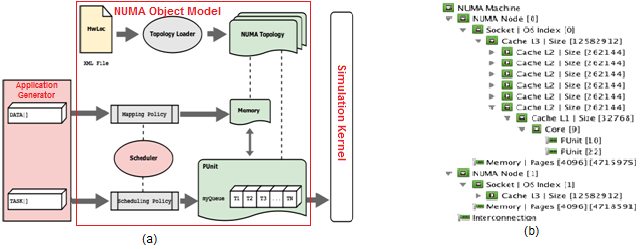
\includegraphics[scale=0.9]{model_sim_numa}
\centering
\caption{NUMA object model structure a- interne b- Arborescence de la topologie}
\label{fig:NUMAMOSIAT}
\end{figure}
%
Un simulateur de haut niveau pour les plateformes multicoeur NUMA (Hihg Level Simulator of Multicore NUMA HLSMN) a été conçu. Sa conception est faite de telle façon qu'elle expose les fonctionnalités de base de la machine MC-NUMA. Sa structure interne est constituée de plusieurs composants interconnectés en fonction de la topologie de la machine cible. Le schéma donné par la figure \ref{fig:NUMAMOSIAT} représente cette conception. 
%\begin{sidewaysfigure}[h]
\begin{figure}[h]
    \centering
    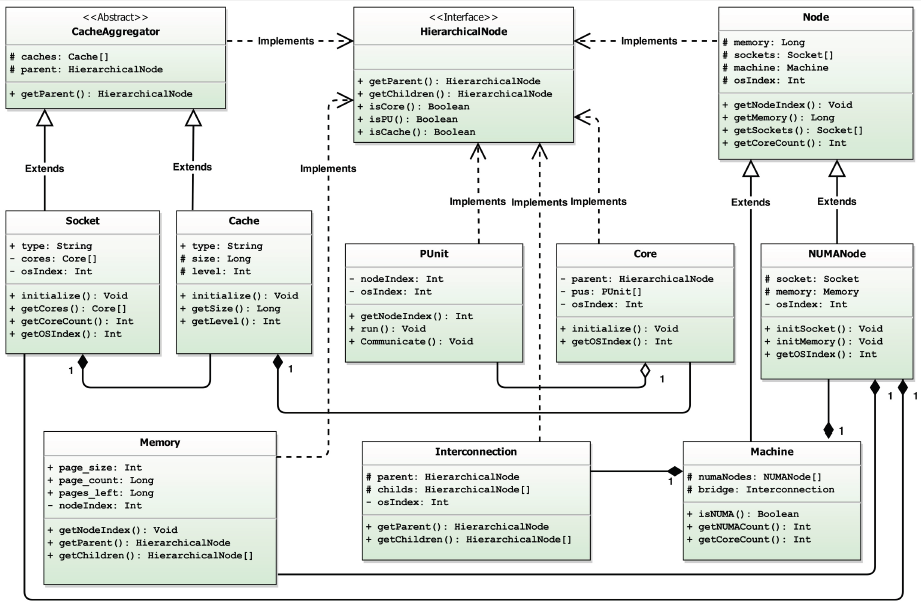
\includegraphics[ scale = 0.65]{om_numa}
    \caption{Architecture du simulateur HLSMN}
    \label{fig:archHLSMN}
\end{figure}
%\end{sidewaysfigure}
\subsubsection{Modèle objet NUMA}
Ce modèle est inspiré de l'outil Xml DTD de Hwloc. Nous effectuons le processus inverse de Hwloc, ces outils génèrent la description basée sur XML d'une plateforme cible réelle à utiliser par l'ordonnanceur. Dans notre cas, nous allons prendre une telle description et construire un modèle d'objet qui correspond à la plateforme cible. La figure \ref{fig:archHLSMN} donne une représentation globale de l'architecture interne de ce simulateur.  Le modèle d'objet se compose de plusieurs modules, y compris:

- \textbf{Machine} : est le module principal à activer pour utiliser le modèle. Il connecte tous les autres modules de manière appropriée en fonction de la description de la topologie.

- \textbf{HierarchicalNode} : est une interface qui résume la structure hiérarchique de cette plateforme. Comme la hiérarchie de la mémoire est structurée comme une arborescence et elle est plus complexe dans NUMA, chaque élément de cette architecture est considéré comme un nœud dans cet arbre (bancs de mémoire, caches, noyau, ...) puis ils partagent les mêmes fonctionnalités d'entités connectées en arbre (accès root ou parent, énumérer la liste de nœuds-fils, notifier la racine ou le parent, ...).

- \textbf{NumaNode} : c'est l'entité la plus importante dans la machine qui modélise l'élément NUMA. Il sera connecté au réseau d'interconnexion et il se comportera seul comme entité SMP.

- \textbf{Socket} : le package processeur contient les unités de calculs (cœurs) et le reste de la hiérarchie mémoire de différents niveaux.

- \textbf{Core} : l'unité de calcul de base qui exécute les threads associés aux tâches d'application.

- \textbf{Interconnexion} : un réseau spécial pour connecter NumaNodes et router les messages entre les différentes entités.

- \textbf{Mémoire} : unités de stockage associées à NumaNode. C'est le stockage local pour ce nœud associé avec une faible latence et une bande passante élevée, contrairement à d'autres nœuds non directement connectés (nœud distant) où la latence est élevée et la bande passante basse.

La figure \ref{fig:archHLSMN} (a) montre les principaux composants de cette partie et expose l'architecture de l'objet NUMA Modèle de HLSMN avec ses composants principaux montrant la relation entre les classes dans le package NUMA. Chaque classe implémente l'interface HierarchicalNode ou étend une autre classe qui l'implémente, de sorte qu'elles héritent des mêmes propriétés et comportements. Sur la base de cette interface, nous pouvons identifier les nœuds-parents et les nœuds-fils dans la hiérarchie en appelant les fonctions getParent() et getChildren() et en récupérant les objets de type HierarchicalNode.
%
\subsubsection{Gestionnaire des topologies}
%
Il est responsable du chargement de la topologie à simuler. Après avoir chargé correctement le fichier associé, il affiche la structure dans la visionneuse de topologie (\ref{fig:archHLSMN} (b)). Ensuite, en fonction de cette structure, il crée le modèle d'objet en instanciant un objet de type Machine et en fait la racine de la hiérarchie. Chaque composant de la topologie possède sa propre classe de représentation qui est initialisée et qui invoque une autre méthode pour créer des sous-éléments ou des enfants dans cet ordre:
%
\subsubsection{Générateur de l'application}
%
Pour exécuter différents scénarios de simulation, nous avons conçu un générateur des applications modèles (Template). Sa tâche consiste à générer des tâches aléatoires en fonction du modèle donné. Le modèle d'application se compose de tâches définies avec des caractéristiques de calcul et la communication doit représenter une classe d'applications parallèles réelles qui partagent un certain profil (application avec plus de calcul et moins de communication ou communication intense) et spécifie les données et le volume nécessaire pendant l'exécution. Selon ce modèle, ce module générera une instance d'application à transmettre comme paramètre au modèle d'objet.
%
\subsubsection{Noyau de simulation}  %\textbf{Exécuteur des politiques}
%
Ce module est le cœur du simulateur. C'est le noyau qui est responsable de la gestion des processus de simulation, de la synchronisation des événements et de la communication entre les entités de simulation. Lors du démarrage du simulateur et après le chargement de la topologie et de la génération de tâches / données (instance), le module de configuration obtient divers types de paramètres sur la machine cible à partir du modèle d'objet, tel que le nombre de processeurs, la taille de la mémoire, les paramètres d'interconnexion tels que le type, la topologie, la bande passante, la politique de routage, etc. et la structure et les détails de l'instance d'application. Ce module essaie de jouer une politique d'ordonnancement choisie sur l'instance donnée de l'application pour prendre les décisions concernant le temps début d'exécution et les nœuds alloués. Ensuite, il mappe les données associées sur les mémoires de nœud en utilisant une autre politique de placement de données choisie. Enfin et lorsque les tâches sont prêtes à être exécutées sur la ressource disponible, l'exécution est lancée sur le nœud alloué et en affectant les données à la mémoire choisie. Il est basé sur la capture des événements survenus sur chaque objet du modèle d'objet, le renvoi et la notification des parties intéressées aux événements survenus. À mesure que les modules fonctionnent simultanément dans ses threads de travail (cœurs, mémoires, interconnexions), il assure la synchronisation et la communication entre eux pour accéder aux ressources partagées (événements de file d'attente, ...).

Comme il est important et critique dans le processus de simulation de garder l'historique, nous avons conçu avec le simulateur, un outil pour enregistrer la trace de la simulation et en collectant les statistiques. 
%====================================================================================
\newpage
\section{Expérimentation tâches indépendantes} \label{etiar}
%
Le scénario de simulation spécifique consiste à configurer les paramètres de l'enviro-nnement de simulation en spécifiant la topologie cible, le modèle d'application pour créer une instance, en choisissant les stratégies d'ordonnancement et de placement à appliquer sur les tâches et les données. Ensuite, nous lançons l'expérimentation en utilisant les paramètres spécifiés. Enfin, nous recueillons les résultats de cette simulation en enregistrant les événements. La dernière étape consiste à analyser les résultats obtenus.
%
\subsection{Configuration de la simulation}
%
Cette étape consiste à définir les informations de configuration utilisées lors du processus de simulation. En combinant les différentes valeurs des paramètres, la configuration obtenue correspond à un scénario d'expérimentation par la suite. Les paramètres les plus importants sont:

- \textbf{Topologie cible}: est définie via le chargeur de topologie en fournissant le fichier de configuration XML de cette topologie.

- \textbf{Modèle d'application}: il est spécifié dans le générateur d'application en donnant le profil de l'application soumise. Ce générateur crée une instance avec le nombre spécifié de tâches avec des données privées prédéfinies et selon le profil spécifié.

- \textbf{Politique ordonnancement/placement}: spécifier quelle stratégie à utiliser pour l'exécution en fonction des politiques/heuristiques implémentées (à évaluer et à tester).
%
\subsection{Expérimentation des scénarios}
%
Dans cette section, nous aborderons le processus d'expérimentation et d'évaluation de certains scénarios de simulation. Le scénario de simulation avec la topologie cible, le modèle d'application des tâches indépendantes de grains de taille moyenne avec moins de communication (opérations de données Read / Write faibles) et l'ordonnancement de type X avec Y comme stratégie de placement représente une expérience qui va mesurer l'impact de combiner ces deux stratégies sur la classe de l'application choisie. Aux fins de cette expérimentation, nous avons mis en œuvre :\\
- \textbf{Politiques d'ordonnancement} : \textit{Round Robin (SRR)} et \textit{Load Balanced (SLL)}\\
- \textbf{Stratégies de placement}: \textit{First Touch (PFT)} et \textit{Round Robin Allocation (PRR)}

Notre expérience consiste à tester toutes les politiques possibles d'ordonnancement et placement combinées avec deux modèles d'application \textbf{T50} et \textbf{T250} (la première contient 50 tâches indépendantes avec ses 50 données associées et la seconde avec 250) cela nous donnera 8 différents scénarios \textbf{[SRR, SLB] $\times$ [PRR, PFT] $\times$ [T50, T250]}. Et, par conséquent, nous sommes intéressés par le temps d'exécution total et le nombre d'accès distant dans chaque scénario.
%
\subsection{Analyse des Résultats}
%
Nous présentons ici la moyenne des résultats après la répétition des expériences qui correspondent à chaque scénario. D’abord une première expérimentation concernant la métrique temps total d'exécution et puis nous montrerons une deuxième mesurant la pénalité NUMA. 
%Lorsque l’on lance les programmes de test, nous obtenons la courbe et le schéma donnés dans les figures 4.5, 4.6 et 4.7.

Le tableau \ref{table:TotalExeTimeSCAB00} donne le temps total d'exécution pour chaque scenario qui est graphique-ment représenté par La figure \ref{fig:TotalExeTimeSCAB}.

Dans les scenarios de 50 tâches, les scenarios configurés avec le placement PFT (6.18, 7.213) donnent un temps total d'exécution meilleur que celui du PRR (7.854, 11.372). Dans les scenarios de 250 tâches, toujours le placement PFT (21.877, 39.084) présente des meilleurs résultats par rapport à l'autre stratégie PRR (25.799, 40.107). En comparant cette fois par rapport à la stratégie d'ordonnancement, nous observons que la politique SRR n'a pas pu dépasser sa concurrente en donnant un temps total d'exécution (25.799, 40.107) nettement supérieur à celui de SLL (21.877, 39.084). 

Le fait de mapper les données d'une tâche selon la stratégie PFT (sur la mémoire du nœud sur lequel elle tourne), cette décision a influencé son temps total d'exécution par rapport PRR (de distribuer les données à tour de rôle sur les mémoires des nœuds de la plateforme). Cela est peut-être dû à un nombre d'accès moins important que celui de PRR puisque chaque tâche charge ses données dans sa mémoire locale si elle est la première à y accéder. Alors ce facteur a réduit la communication distante donc il a permis de terminer tôt la tâche et en conséquence  de donner un temps total d'exécution inférieur par rapport la distribution RR qui ne tient pas en compte la source de la requête d'allocation mémoire (quelle tâche a demandé cette donnée\?). C'est pourquoi il va générer plus de communication distante donc retarder la terminaison de la tâche et donner un $C_{max}$ important.
%
\begin{table}[h!]
\centering
\begin{tabular}{| c | c | c | c | c |} 
\hline
Tasks/Policy	& PRR-SRR 	& PRR-SLL 	& PFT-SRR 	& PFT-SLL 	\\ [0.5ex] \hline
50 Tasks 		& 7.854 		& 11.372 		& 6.18			& 7.213 		\\ [0.5ex] \hline
250 Tasks		& 25.799 		& 40.107 		& 21.877 		& 39.084 		\\ [0.5ex] \hline
\hline
\end{tabular}
\caption{Temps total d'exécution de chaque scénario 50/250 tâches}
\label{table:TotalExeTimeSCAB00}
\end{table}

La figure \ref{fig:RemoteAccessMemTraceAB} montre graphiquement les accès distants aux données effectués par les tâches résidants sur les nœuds de la plateforme. Comme prévu, Les 50 tâches ont un nombre d'accès distants moins important que les 250 tâches. En comparant maintenant entre les stratégies testées, le nombre des accès distant pour PRR-SRR et PFT-SRR est nettement inferieurs (moins de lignes colorées) à celui de PRR-SLL et PFT-SLL pour les deux scénarios. (La densité des lignes en vert et rouge est faible par rapport la densité des lignes en bleu et jaune). 

Ce scénario a donné un résultat qui n'était pas prévu puisque la politique PFT s'est comportée comme l'autre politique PRR en générant un nombre similaire d'accès distant malgré qu'elle charge les données dans la mémoire locale de la tâche demandeuse. Une interprétation possible est qu'il y a assez de tâches qui partagent la même donnée et puisque il n'y a pas de  migration de tâche alors la première qui demande la donnée elle l'obtient en local mais le reste doit faire une communication distante pour l'utiliser (en lecture ou écriture).

%
\begin{figure}[h]
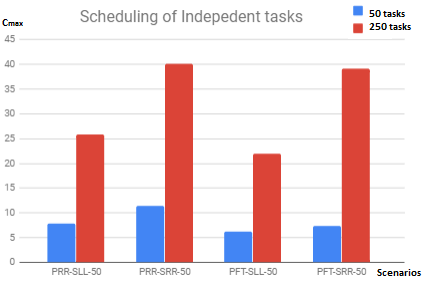
\includegraphics[scale=0.9]{result_numa022}
\centering
\caption{Temps total d'exécution pour chaque scénario (a) 50 tâches (b) 200 tâches}
\label{fig:TotalExeTimeSCAB}
\end{figure}
%
\begin{figure}[h]
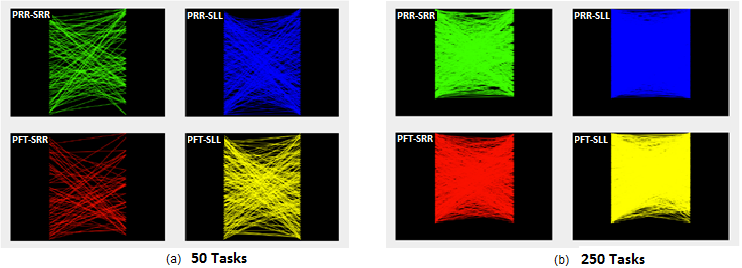
\includegraphics[scale=0.80]{result_numa01}
\centering
\caption{Trace des acces mémoire distants (a) 50 tâches (b) 200 tâches}
\label{fig:RemoteAccessMemTraceAB}
\end{figure}
%

%
%====================================================================================
\newpage
\section{Expérimentation tâches dépendantes DAG} \label{etdar} 
%
Dans cette section nous allons expérimenter notre heuristique. Tout d'abord, un scenario d'expérimentation sur des applications parallèles de différente configuration (DAGs dont le nombre de tâches et structures différentes) est réalisé en mesurant le temps total d'exécution sur des plateformes NUMA de différentes architectures. Ensuite le même scenario d'expérimentation est répété pour les même applications parallèles mais cette fois on s'intéresse à la pénalité NUMA.
%
\subsection{Configuration de la simulation}
%
Afin de configurer les scénarios de simulation, nous présentons les différentes rubriques et les options à paramétrer :\\
\textbf{Topologie simulée} :\\
- \textit{Plateforme configuration Nombre de nœuds/cœurs (xNyC)}\\
- \textit{Réseaux ICN} : La matrice des distances entre les nœuds est donnée comme paramètre de simulation.
\\
\textbf{Jeu de Test} \\
Ce jeu de test est choisi parmi l'ensemble des DAGs au \textbf{format STG} \cite{STG16} qui constitue une référence pour le test des problèmes utilisant des DAGs. Le format STG a été enrichi en ajoutant un champ appelé motif d'accès mémoire spécifique pour les architectures NUMA. Le listing suivant donne un exemple d'un DAG codé en STG avec l'extension motif d'accès. La notation utilisée est DAGXx ou Xx est le nombre de tâches du DAG utilisé (DAG50 contient 50 tâches).
%
\begin{Verbatim}[formatcom=\color{blue}]
//DAG050 au format STG de 50 Tâches et avec sa précédence
	50
	00	00	0	-	S;0;20;R;1;50;W;0;30;E;1;0
	01	09	1	0	S;2;30;R;3;20;W;2;50;E;3;0
	02	04	1	0	S;4;50;R;5;30;W;4;20;E;5;0
	03	03	1	0	S;6;20;R;7;50;W;6;30;E;7;0
	04	06	1	0	S;0;20;R;1;50;W;0;30;E;1;0
	05	04	1	1	S;2;30;R;3;20;W;2;50;E;3;0
	06	03	1	5	S;4;50;R;5;30;W;4;20;E;5;0
	07	03	1	0	S;6;20;R;7;50;W;6;30;E;7;0
	08	08	1	6	S;0;20;R;1;50;W;0;30;E;1;0
	09	09	1	0	S;2;30;R;3;20;W;2;50;E;3;0
	10	02	3	2;6;8  S;4;50;R;5;30;W;4;20;E;5;0
	11	01	1	9	S;6;20;R;7;50;W;6;30;E;7;0
	12	10	1	0	S;0;20;R;1;50;W;0;30;E;1;0
........
\end{Verbatim}
%
\begin{table}[h!]
\centering
\begin{tabular}{| c | c | c | c | c |} 
\hline
Task.id 		& Length 	& Number of Prec 	& Precedences 	& Task Data access pattern \\ [0.5ex] \hline
10 			& 2 	& 3 		& 2;6;8 		& S;4;50;R;5;30;W;4;20;E;5;0 \\ [0.5ex] \hline
\end{tabular}
\caption{Ligne tâche dans le fichier DAG au format STG étendu}
\label{table:TB_2_22220}
\end{table}
%
Le DAG décrit par ce fichier a 50 tâches dont la tâche 0 est la \textbf{tâche d'entrée}, chaque ligne contient l'\textbf{identifiant} de la tâche, sa \textbf{longueur}, le \textbf{nombre de ses prédécesseurs}, la \textbf{liste de ses prédécesseurs} et à la fin le champ supplémentaire pour le cas de NUMA ou en spécifiant le \textbf{motifs d'accès} aux données. Ce motif décrit le schéma d'exécution de sa tâche, il commence avec \textbf{S (start)} en spécifiant les données à charger ou lancement de la tâche ensuite le pourcentage des instructions exécuter par le cœur par rapport au nombre total des instructions de la tâche suivi par une communication soit \textbf{lecture (READ/LOAD)} ou \textbf{écriture (WRITE/STORE)} en spécifiant la donnée concernée et enfin l'étape de la finalisation \textbf{E (end)} de l'exécution de la tâche en sauvegardant les données avant sa terminaison.
\\
\textbf{Heuristiques simulés Ordonnancement}\\   %- \textbf{UMA}   : sur la plateforme UMA \\
- \textit{NXH}   : sur la plateforme NUMA sans Horizon d'exécution \\
- \textit{WXH}  : sur la plateforme NUMA avec l'heuristique Horizon d'exécution X-VHFU
\\
\textbf{Placement}\\
- \textit{AoFT} : Affinity-on-First-Touch
\\
\textbf{Métriques mesurées}\\  %- \textbf{NR} : NUMA ratio\\
- \textit{Cmax} : Temps Total d'exécution\\
- \textit{NR} : Penalité NUMA
%--------------------------------------------------------------------------------
\subsection{Expérimentation des scénarios}
%
Nous allons réaliser deux scénarios qui ont la même configuration d'expérimentation. L'objectif visé dans le premier est de mesurer le temps total d'exécution et dans le deuxième sera la pénalité NUMA.\\
%
\textbf{Scenario 01} :\\
La configuration de ce scénario est la suivante : \\
- \textbf{PF} : 8N2C, 4N4C, 8N1C, 4N2C, 2N4C, 2N2C\\
- \textbf{DAG} : DAG25, DAG50, DAG75, DAG100, DAG125, DAG150\\
- \textbf{S/P} : NXH, WXH / AoFT\\
- \textbf{Métrique mesurée} : Temps Total d'exécution\\
%
\textbf{Scenario 02} :\\
La configuration de ce scénario est la suivante : \\
- \textbf{PF} : 8N2C, 4N4C, 8N1C, 4N2C, 2N4C, 2N2C\\
- \textbf{DAG} : DAG25, DAG50, DAG75, DAG100, DAG125, DAG150\\
- \textbf{S/P} : NXH, WXH / AoFT\\
- \textbf{Métrique mesurée} : Penalité NUMA\\
%
\subsection{Analyse des Résultats}
%
\textbf{Scenario 01} :\\
%
La figure \ref{fig:fig100400x} donne un exemple d'une expérience effectuée en exécutant un DAG STG de 100 tâches sur une plateforme de 4 nœuds et 2 cœurs sur chaque nœuds. La figure représente le diagramme de GANT de l'exécution des tâches sur les cœurs ($P_i$) des nœuds de la plateforme. Nous pouvons voir l'affectation de chaque tâche, sa date début d'exécution, sa fin d'exécution et son temps d'exécution. Les contraintes de précédence imposent la précédence et une synchronisation entre les tâches dépendantes (tâches filles et mères) qui se manifestent comme un temps d'attente (de communication inter tâches $C_i$) de la terminaison des tâches précédentes pour lancer une tâche fille. $C_{max}$ est le temps maximum enregistré par la dernière tâche du DAG pour finir.
%
\begin{figure}[h!]
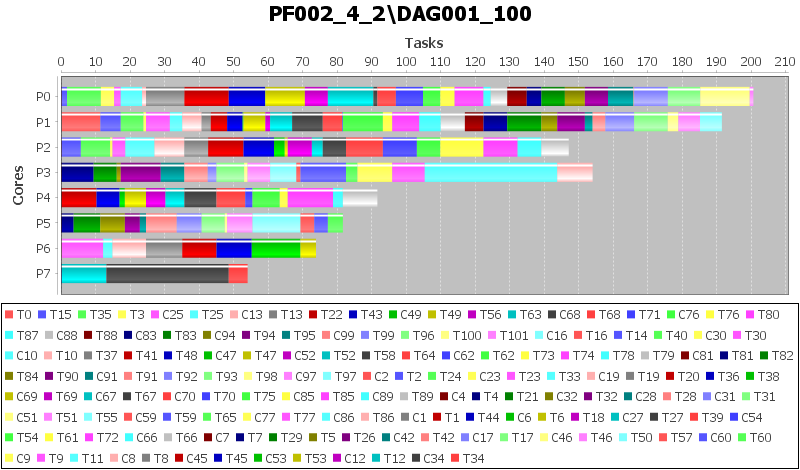
\includegraphics[scale=0.75]{dag1004}
\centering
\caption{Diagramme GANT résultat de l'exécution d'un scénario}
\label{fig:fig100400x}
\end{figure}
%
%
\begin{figure}[h!]
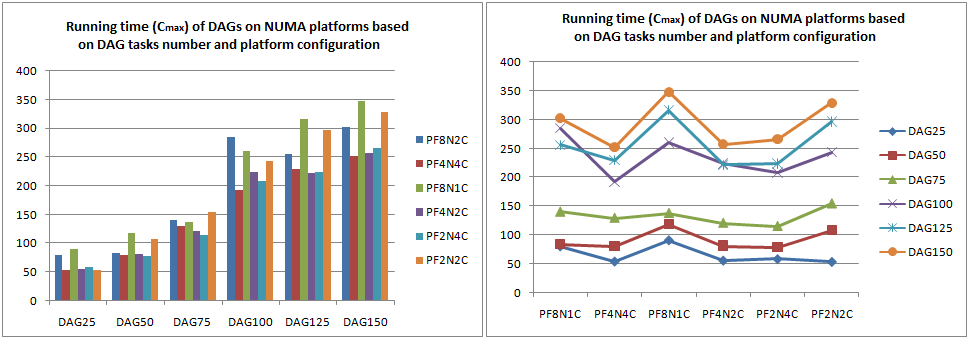
\includegraphics[scale=0.60]{STATISPHD001}
\centering
\caption{Scénario d'expérimentation pour mesurer $C_{max}$}
\label{fig:fg10200x}
\end{figure}
%
La figure \ref{fig:fg10200x} donne le $C_{max}$ associé à chaque DAG ordonnancé sur la plateforme cible. Il montre que pour les DAGs qui ont plus de 100 tâches le $C_{max}$ dépasse 200 unité temps sur toute les plateformes. Mais pour les DAGs dont le nombre de tâches est inferieur à 75 cette valeur reste au dessous de 150 unités temps sur les plateformes testées.

Dans ce premier scénario, Les statistiques collectées concernent le temps total d'exécution en fonction de la politique utilisée pour ordonnancer les tâches (en utilisant l'heuristique XH-VHFU ou non). La stratégie XH est basé sur le principe de la sélection de la tâche à exécuter qui va élargir l'horizon d'exécution après sa sélection, par contre la stratégie classique sélectionne la première qui est en-tête de la liste de tâches prêtes.

La figure \ref{fig:fig1045} donne les détails de l'expérimentation du scénario courant dont la métrique mesurée est le temps total d'exécution pour l'ensemble des DAGs pour les deux cas avec activation XH ou non. En fonction de chaque DAG, \\
\\
- DAG25 : 4 cas sur 6 que les tests avec XH activé dépassent ceux sans XH avec une moyenne d'écart de 4 \% et les valeurs des deux tests s'étalent sur la plage 55 à 88.\\
- DAG50 : 5 cas sur 6 que les tests avec XH activé dépassent ceux sans XH avec une moyenne d'écart de 6 \% et les valeurs des deux tests s'étalent sur la plage 75 à 112.\\
- DAG75 : 5 cas sur 6 que les tests avec XH activé donnent des valeurs supérieures aux valeurs du tests ans XH avec une moyenne d'écart de 7\% et les valeurs des deux tests s'étalent sur la plage 110 à 180.\\
- DAG100 : 5 cas sur 6 que les tests sans XH activé dépassent ceux avec XH avec un écart faible dont la moyenne est -3 \% et les valeurs des deux tests s'étalent sur la plage 190 à 290.\\
- DAG125 : 5 cas sur 6 que les tests avec XH activé dépassent ceux sans XH avec une moyenne d'écart de 4\% et les valeurs des deux tests s'étalent sur la plage 215 à 355.\\
- DAG150 : 4 cas sur 6 que les tests avec XH activé dépassent ceux sans XH avec une moyenne d'écart de 3 \% et les valeurs des deux tests s'étalent sur la plage 255 à 360.

%\begin{table}%[h!]
%\centering
%\begin{tabular}{| c | c | c | c | c | c | c |} 
%\hline
%DAG/PF 	& PF8N2C 	& PF4N4C 	& PF8N1C 	& PF4N2C 	& PF2N4C  	& PF2N2C \\ [0.5ex] \hline
%25 		& 80.35 	& 54.24 		& 90.83 		& 55.67 		& 58.34  		& 53.49 \\ [0.5ex] \hline
%50 		& 83.43 	& 80.39 		& 117.93 		& 81.07 		& 79.04  		& 107.76 \\ [0.5ex] \hline
%75 		& 140.37 		& 129.72 		& 138.17 		& 120.98 		& 115.25  		& 154.95 \\ [0.5ex] \hline
%100		& 285.25 		& 192.37 		& 260.72 		& 224.07 		& 208.67  		& 243.54 \\ [0.5ex] \hline
%125		& 256.38 		& 229.93 		& 316.39 		& 222.07 		& 224.43  		& 296.56 \\ [0.5ex] \hline
%150		& 802.53 		& 251.84 		& 348.24 		& 257.11 		& 265.26  		& 328.80 \\ [0.5ex] \hline
%\hline
%\end{tabular}
%\caption{charge moyenne de la plateforme NUMA x3}
%\label{table:TB_2_1}
%\end{table}
%
Les résultats présentés montrent que l'intégration de heuristique XH a donnée dans la plupart des cas (en moyenne 4 cas sur 6) des écart positif en améliorant le temps total d’exécution entre 3\% à 6\% en moyenne par rapport à la stratégie normale. La découverte de l'horizon au fur et a mesure de l'avancement du processus de l'ordonnancement permet de guider le processus de la prise de décision pour sélectionner la tâches courante à exécuter en exploitant les informations de la visibilité des tâches non encore exécutées en récompensant le manque de l'information concernant la longueur de tâches et les données et le volume échangés entre les tâches.\\
%
\afterpage{
\clearpage 
\thispagestyle{empty}
\begin{landscape}
\begin{center}

\begin{figure}[h!]
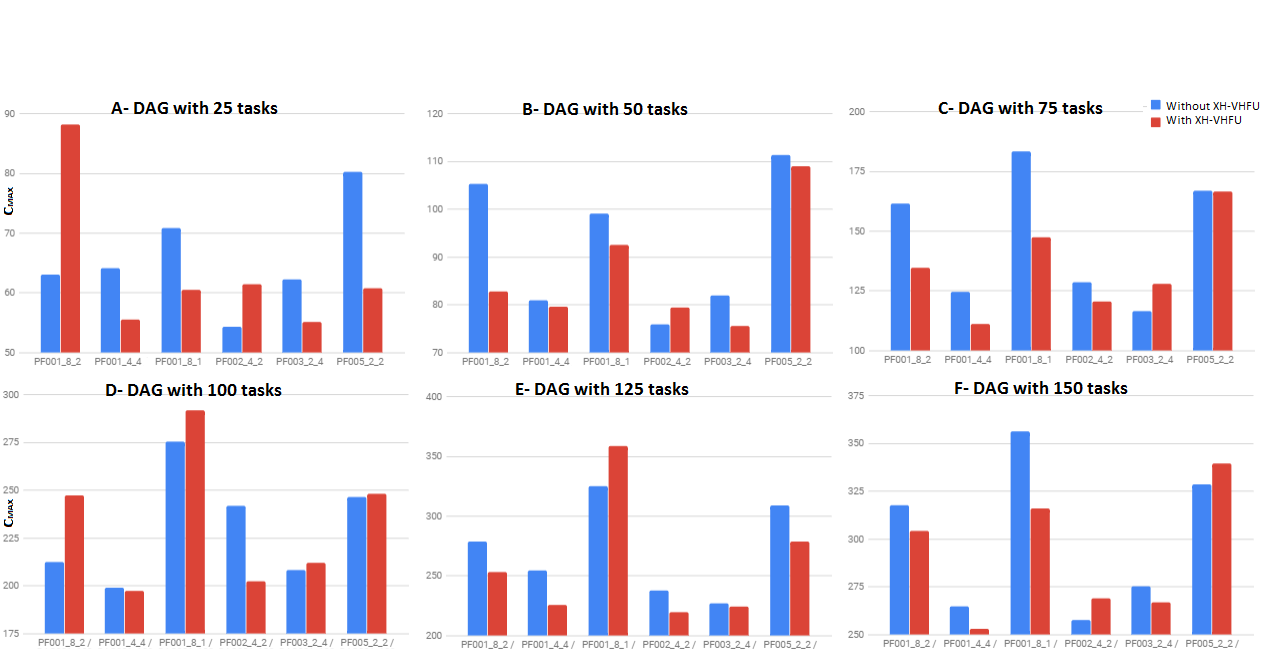
\includegraphics[scale=0.75]{hx002-00}
\centering
\caption{Temps total d'exécution mesuré pour le scénario joué}
\label{fig:fig1045}
\end{figure}

\end{center} 
\end{landscape}
\clearpage
}
%\newpage
\textbf{Scenario 02} :\\
Dans ce deuxième scénario, Les statistiques collectées concernent la pénalité NUMA (le rapport entre le nombre des accès distants par rapport  le nombre des accès locaux, nous allons utiliser un facteur équivalent le pourcentage des accès distants par rapport au nombre total d'accès) en fonction de la politique utilisée pour ordonnancer les tâches (en utilisant l'heuristique XH-VHFU ou non). Lors de l'exécution du code d'une tâche, si l'instruction exécutée est un chargement/une sauvegarde (LOAD/STORE) alors une requête qui correspond à cette opération est faite au système mémoire si la donnée sollicitée est sauvegardé dans la mémoire du nœud exécutant sa tâche alors c'est accès local. Le cœur exécutant adresse cette requête au contrôleur mémoire local qui se charge de récupérer la donnée. Par contre si l'emplacement est sur une mémoire distante alors l'accès est distant. 

Le tableau \ref{table:TB_2_2222} donne le nombre des accès locaux et distants pour l'ensemble des DAGs testés et les valeurs de la pénalité associées pour la première option sans l'utilisation de l'heuristique proposée. Pour la plateforme PF2N2C, la plage des valeurs enregistrées est entre 74\% et 79\%.  Le deuxième tableau \ref{table:TB_2_2223} utilise le même paramètre sauf que cette fois la politique configurée est l'heuristique XH-VHFU. Pour la même plateforme PF2N2C, la plage des valeurs enregistrée est entre 70\% et 78\%. 
Dans les deux cas, le nombre des accès distants dépasse 70\% qui est un pourcentage élevé et un indicateur d'une mauvaise localité malgré l'utilisation de la stratégie AoFT. La deuxième série de tests (avec heuristique) a relativement des valeurs inferieures à par rapport à la première série (sans heuristique), mais cette amélioration est minime et n'est pas significative pour réduire l'impact de cette pénalité sur la performance système.

La figure \ref{fig:fig10450} donne Les détails de l'expérimentation du scénario courant dont la métrique mesurée est la pénalité NUMA pour l'ensemble des DAGs pour les deux cas avec activation XH ou non. En fonction de chaque plateforme, \\
\\
- PF2N2C : 5 cas sur 6 que les tests avec XH activé dépassent ceux sans XH avec une moyenne d'écart de 4 \% et les valeurs des deux tests s'étalent sur la plage 70\% à 78\%.\\
- PF2N4C : 4 cas sur 6 que les tests avec XH activé dépassent ceux sans XH avec une moyenne d'écart de 2 \% et les valeurs des deux tests s'étalent sur la plage 80\% à 89\%.\\
- PF4N2C : 4 cas sur 6 que les tests avec XH activé donnent des valeurs légèrement supérieure aux valeurs du tests ans XH avec une moyenne d'écart de -2 \%  car les deux autre cas présentent un écart important et les valeurs des deux tests s'étalent sur la plage 80\% à 89\%.\\
- PF8N2C 3 cas sur 6 que les tests sans XH activé dépasse ceux avec XH avec un écart remarquable dont la moyenne est -3 \% et les valeurs des deux tests s'étalent sur la plage 82\% à 92\%.\\
- PF8N1C 3 cas sur 6 que les tests avec XH activé dépassent ceux sans XH avec une moyenne d'écart de 2 \% et les valeurs des deux tests s'étalent sur la plage 82\% à 89\%.\\
- PF4N4C 3 cas sur 6 que les tests avec XH activé dépassent ceux sans XH avec une moyenne d'écart de 1 \% et les valeurs des deux tests s'étalent sur la plage 82\% à 91\%.

Les résultats présentés montrent que l'impact de l'intégration de heuristique XH n'a pas été significatif pour réduire le nombre d'accès distant  certes dans 4 tests sur 6 elle a contribué à réduire cette pénalité mais cette réduction n'est pas suffisante vu que la plage des valeurs reste très importante et l'écart trouvé relativement faible. 
%
\begin{table}%[h!]
\centering
\begin{tabular}{| c | c | c | c | c | c | c |} 
\hline
Access 		& DAG25 	& DAG50 	& DAG75 	& DAG100 	& DAG125  	& DAG150 \\ [0.5ex] \hline
Local 			& 25 	& 54 		& 64 		& 108 		& 110  		& 161 \\ [0.5ex] \hline
Remote 		& 83 	& 154 		& 243 		& 300 		& 398  		& 447 \\ [0.5ex] \hline
Rate 		& 77 		& 74 		& 79 		& 74 		& 78  		& 74 \\ [0.5ex] \hline
\hline
\end{tabular}
\caption{Pénalité NUMA pour chaque instance DAG sans XH-VHFU}
\label{table:TB_2_2222}
\end{table}

\begin{table}%[h!]
\centering
\begin{tabular}{| c | c | c | c | c | c | c |} 
\hline
Access 		& DAG25 	& DAG50 	& DAG75 	& DAG100 	& DAG125  	& DAG150 \\ [0.5ex] \hline
Local 			& 28 	& 62 		& 74 		& 101 		& 139  		& 167 \\ [0.5ex] \hline
Remote 		& 80 	& 146 		& 234 		& 307 		& 369  		& 441 \\ [0.5ex] \hline
Rate 		& 74 		& 70 		& 76 		& 75 		& 73  		& 73 \\ [0.5ex] \hline
\hline
\end{tabular}
\caption{Pénalité NUMA pour chaque instance DAG avec XH-VHFU}
\label{table:TB_2_2223}
\end{table}
%
\afterpage{
\clearpage
\thispagestyle{empty}
\begin{landscape}
\begin{center}

\begin{figure}[h!]
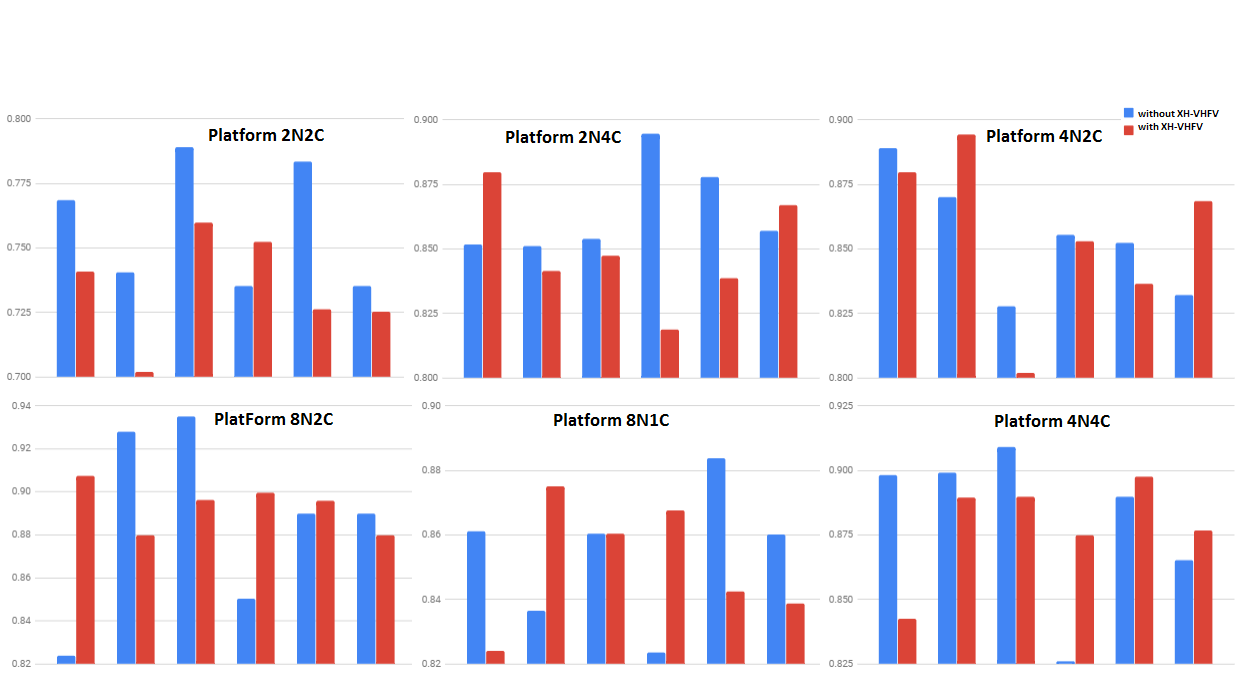
\includegraphics[scale=0.75]{rla_00}
\centering
\caption{Pénalité NUMA mesuré pour scénario joué}
\label{fig:fig10450}
\end{figure}

\end{center} 
\end{landscape}
\clearpage
}   
%====================================================================================
\newpage
\section{Expérimentation Equilibrage de charge} \label{eecar}
%
Dans cette section nous allons expérimenter notre heuristique concernant l'équilib-rage de charge lors de l'exécution des tâches sur une plateforme NUMA. Dans un premier temps, un scenario d'expérimentation configuré sans option d'équilibrage de charge. Dans ce scénario, une série de tâches est lancée sur une plateforme NUMA et durant le déroulem-ent de l'exécution nous allons collecter l'information sur la charge courante sur chaque nœud à la fin nous calculons la charge moyenne sur le système. Un deuxième scénario est configuré avec l'activation de l'option de l'équilibrage de charge en utilisant la stratégie proposée dans de cette thèse à savoir le vol de travail basé sur la distance et adapté à l'architecture NUMA.%
\subsection{Configuration de la simulation}%
La configuration simulée est la suivante :\\
- \textbf{Topologie simulée} : Plateforme configuration Nombre de nœuds/cœurs (4N1C)\\  %8N2C, 4N4C, 8N1C, 4N2C, 2N4C, 2N2C\\
- \textbf{Jeu de Test} : Une série de 1500 tâches\\
- \textbf{Heuristiques simulés Equilibrage de charge} : sans /avec vol de travail basé sur la distance\\
- \textbf{Métriques mesurées} : La charge moyenne\\  %- \textbf{NR} : NUMA ratio\\
%--------------------------------------------------------------------------------
\subsection{Expérimentation des scénarios}
%
\textbf{Scenario 01} 

Dans ce scenario, l'expérimentation est faite sur une plateforme NUMA de quatre nœuds et un cœur pour chaque nœud avec 1500 tâches indépendantes en la paramétrant sans ou avec une stratégie de l'équilibrage de charge.  Pour cette stratégie, nous avons testé dreux variantes basées sur le vol de travail celle la classique (dont la sélection des victimes est aléatoire) et celle l'adaptée à NUMA basée sur la distance. Le but de cette expérimentation est d'évaluer la charge instantanée au cours de l'exécution et sa charge moyenne.\\
1- Topologie simulée : \textbf{4N1C}\\
2- Jeu de Test : \textbf{1500 tâches}\\
3- Heuristiques simulés Equilibrage de charge : sans ou avec vol de travail (\textbf{NWS}, \textbf{WWS})\\ 
4- Métriques mesurées : \textbf{AL} la charge moyenne

Une série de test sur 1500 tâches est lancée en mesurant instantanément la charge sur chaque nœud de la plateforme et à la fin 
nous calculons la charge moyenne. 

Dans un premier temps, la stratégie de l'équilibrage de charge est désactivée. \\
- Heuristiques simulés Equilibrage de charge : - \textbf{NLB} sans vol de travail

Ensuite un deuxième lot de test avec la même configuration est lancé en utilisant le vol de travail classique pour équilibrer la charge. \\
- Heuristiques simulés Equilibrage de charge : - \textbf{CWS} avec vol de travail classique\\

Enfin un troisième lot de test avec la même configuration est lancé mais cette fois en activant l'équilibrage de charge utilisant l'heuristique vol de travail basée sur la distance adaptée à NUMA. \\
3- Heuristiques simulés Equilibrage de charge : - \textbf{dbANWS} avec vol de travail Adapté NUMA basé sur la distance\\

L'évolution de la charge instantanée sur les nœuds correspond à ce scénario est présentée par la figure \ref{fig:xws01}. Le cas A représente le scénario sans l'utilisation du vol de travail et le cas B active cette option la variante basé sur la distance adaptée NUMA. 
%
\begin{figure} %[h!]
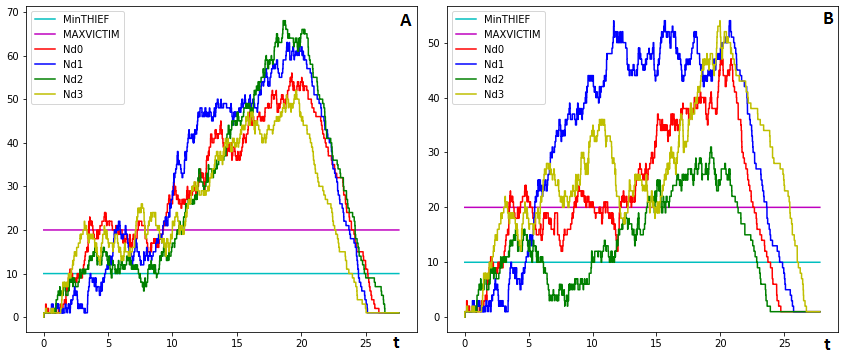
\includegraphics[scale=0.70]{xws01}
\centering
\caption{Charge instantanée des nœuds avec/sans vol de travail adapté NUMA}
\label{fig:xws01}
\end{figure}
%
\subsection{Analyse des Résultats}
%
La figure \ref{fig:fg101} représente l'évolution de la charge moyenne des nœuds de la plateforme NUMA. La partie A concerne les tests sans équilibrer la charge. Dans la partie B, le vol de travail classique est utilisé comme stratégie pour équilibrer la charge, et la dernière partie C, nous avons remplacé la stratégie vol de travail classique par notre variante adaptée NUMA.   
%
\begin{figure}[h!]
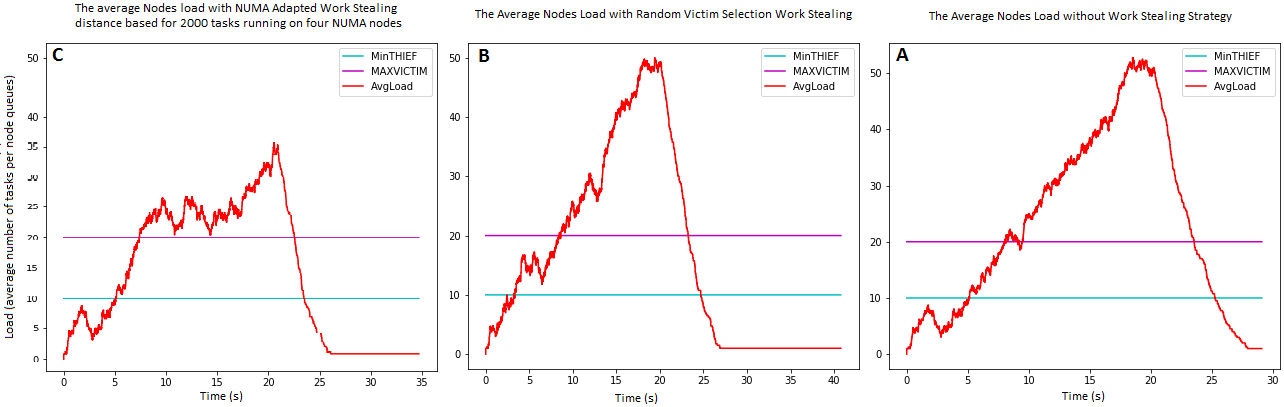
\includegraphics[scale=0.45]{myfigs9-f}
\centering
\caption{Charge moyenne de la plateforme NUMA 4 noeuds}
\label{fig:fg101}
\end{figure}
%
\\
Dans ce scénario, les statistiques collectées concernent la charge sur les noeuds en fonction de la politique d'équilibrage de charge  utilisée (sans vol de travail, avec vol travail aléatoire et avec vol travail adapté NUMA). Apres la soumission d'un lot de taches à un ordonnanceur à exécuter, nous avons enregistré la charge instantanée sur chaque noeud. Selon la figure \ref{fig:xws01}, l'évolution de la charge sur les noeuds s'est accelérée pour atteindre un pic maximum de 70 taches et un pic minimum de 50 taches pour le cas sans utilisation de vol de travail. Par contre, lorsque nous avons activé cette option un pic maximum 52 taches et minimum de 28 taches ont été enregistré. Nous constatons que cette option a redistribué la charge de la plateforme en évitant une surcharge sur les noeuds au meme moment. La figure \ref{fig:fg101} montre que les charges moyennes enregistrées avec les deux premieres strategies sont presque similaires dont l'évolution est croissante jusqu'à un pic maximum de 50 taches. Par contre, la stratégie vol de travail basé sur la distance a donné une charge moyenne plus stable et beaucoup plus inferieure que la précedente. Avec un pic de 35 taches maximum et répartiton temporelle accepatble. Une amélioration moyenne de la charge de 15\% (pic maximum).
%====================================================================================
\newpage
\section{Conclusion}\label{conc}
%
Dans ce chapitre, nous avons conçu et mis en œuvre HLSMN un simulateur de haut niveau de plateforme multicouches NUMA qui nous permet de nous concentrer sur l'aspect algorithmique des politiques et de masquer les détails de bas niveau. HLSMN expose le modèle NUMA avec la hiérarchie des nœuds, des interconnexions et des mémoires, permet d'implémenter et de tester différentes politiques d'ordonnancement et de placement de données, d'exécuter des processus de simulation et de générer les statistiques concernant l'exécution des applications à base des tâches (le temps d'exécution total des tâches et la pénalité NUMA comme facteurs les plus importants dans un tel contexte). 

Sur la base de ces facteurs, nous avons utilisé ce simulateur pour mesurer l'impact de la combinaison des différentes stratégies d'ordonnancement et de placement (round robin et first touch, ...) des tâches indépendantes de la performance globale du système en terme de temps d'exécution total et de nombre de mémoire d'accès à distance. 

La deuxième partie est consacrée au test et validation de nos heuristiques proposées, Pour le premier lot des scénarios pour expérimenter l'horizon d'exécution étendu, nous avons choisit une série de DAG de taille et structure différentes et nous avons simulé le processus de l'ordonnancement sur des plateformes de topologie différente afin de mesurer le gain de cette approche en fonction des métrique classique le temps total d'exécution et la pénalité NUMA. Pour la première métrique, l'horizon d'exécution étendu a donné un $C_{max}$ inférieur à celui de l'approche ordinaire mais malheureusement ces résultats sont relativement faibles (ne dépassent pas 10\%)  dans la plus part des scénarios. Pour la deuxième métrique, l'horizon d'exécution étendu n'a pas pu améliorer la pénalité NUMA en donnant un taux NUMA presque similaire à celui de l'approche ordinaire pour la plus part des scénarios.

Pour le deuxième lot des scénarios pour expérimenter le vol de travail basé sur la distance, nous avons soumis à cet algorithme un lot de tâches (plus de 1000 tâches indépendantes) et nous avons simulé l'exécution des tâches sur des plateformes de topologie différente afin de mesurer le gain de cette approche en fonction des métrique classique la charge des nœuds. Pour cette métrique, le vol de travail basé sur la distance a donné un bon écart en améliorant la charge par rapport celle  des approches ordinaire (sans équilibrage de charge) ou celle en utilisant le vol de travail aléatoire. Ces résultats sont relativement bons (dépassent 15\% en moyenne).

	\chapter{Conclusion et perspectives}\label{chapter:concusion}
%
Dans le cadre de cette thèse, nous avons étudié le problème de l'ordonnancement des applications parallèles décrites par un graphe de tâches DAG qui s'exécutent sur la plateforme à accès mémoire non uniforme NUMA dont les tâches partagent et échangent des données. En plus de l'aspect ordonnanccement des tâches et l'allocation de processeurs / coeurs aux tâches, un deuxieme aspect qui se manifeste dans ce contexte est le placement des données des tâches sur les mémoires des noeuds puisque la cible est non unforme et asymmétrique pour l'opération des accès mémoire. Cette asymmétrie qui se manifeste par un temps d'accès mémoire different et non néglegeable  pour les données d'une tâches qui résident sur une mémoire d'un noeud différent de celui sur lequel la tâche tourne.

Cet ordonnancement et placement dynamique nous imposent une connaissance impar-faite des conditions d’exécution (nous ne connaissons pas la durée de chaque tâches, le volume exacte des données  échangées, certains paramètres de la plateforme d'exécution). 
En pratique, ce manque d’informations affaiblit fortement les performances des différents algorithmes envisageables.
%
%Comme nous avons cité au début que les principaux défis sur les plates-formes NUMA pour ordonnancer une application parallèle décrite par un graphe de tâches dépendantes acyclique (DAG) sont :
%
%1- Réaliser la bonne allocation tâche/thread-nœud (Trouver l'ordre optimal pour exécuter les tâches de ce DAG sur les nœuds de la plate-forme).
%
%2- Réaliser le bon placement donnée-thread/mémoire-nœud (Mapper les données de telle façon de réduire la latence des accès mémoire et de maximiser la bande passante). 
%
%3- Equilibrer la charge entre les cœurs/nœuds de calculs.
%
%4- Garder certaine proximité spatiale et temporelle entre les tâches dépendantes  lors de l'exécution.
%
%Afin d'entamer un travail de recherche sur ce problème, nous avons fixé au début certains objectif qui nos permettent fixer le cadre du travail. Permis ces objectifs :
%
%1- Optimiser l'ordonnancement des applications parallèles à base de tâches dépendantes sur l'architecture NUMA.%
%
%2- proposer des mécanismes efficaces pour le placement de tâches et de données, améliorant la localité des accès à la mémoire ainsi que les performances systèmes, en optimisant le placement des données associes aux tâches. (augmenter la localité des accès aux données et ainsi de réduire la la pénalité NUMA)
%
Nous avons cherché à travers notre travail à tirer parti de la moindre information disponible pour réduire l’impact de la pénalité NUMA au maximum. Afin de réaliser ces objectifs, nous avons proposé des heuristiques qui visent à améliorer ces deux processus dans ce contexte. 

La première idée était de collecter, au début de l'exécution, plus d'informations prove-nant de l’application parallèle à exécuter et de la plateforme cible et d'utiliser cette information pour guider le processus de l'ordonnancement et le placement (la structure DAG de l'application, la topologie de la plateforme,..). A chaque instant ou un évenement se produit en changeant l'état d'exécution (le début/la fin de l'exécution d'une tâche, déclencher un accès mémoire (R/W),..), l'information collectée est mis à jour.   
%Par la suite, nous rappelons les résultats que nous avons obtenus, les limites de notre travail, ainsi que les perspectives que nous envisageons. Nous présentons ensuite les apports de notre recherche, avant de conclure.
%
\section{Résultats}
%
Nous avons réalisé un ensemble d’expériences testant les algorithmes proposés via la simulation. 
Nous avons mis en évidence la réduction de la pénalite NUMA qui se traduit effectivement par une amélioration des temps total d'exécution. 
Enfin, nous avons montré que l’utilisation de vol de travail basé sur la distance permet réellement d’étendre le champs d’application du vol de
travail aléatoire vers des platesformes hiérarchique NUMA.

Le premier lot d'expériences, c'était l'ordonnancement des tâches indépendantes en combinant les politiques ordonnancement et placement classiques juste pour mesurer l'éffet de cette combinaison sur la pénalité NUMA et son impact sur le temps total d'exécution.
Ces expériences réalisées montrent que certaines combinaison aident à amélio-rer la premiere métrique $C_{max}$ par contre elle échoue à réduire la pénalite (le cas FFLB) et l'inverse pour d'autres cas (RRFT).

Le deuxieme scénario est de tester et valider nos propres heuristiques. Notre travail de simulation se divise en deux
parties. \\
- La première tente d'évaluer l'heuristique horizon d'exécution étendu sur un DAG; \\
- La seconde quant à elle tente de valider le vol de travail basé sur la distance. 

%Les heuristiques simulées ont montré que certains objectifs fixés ont été atteints. 
Nous avons pu exploiter certaines informations collectées à différents niveau pour guider le processus de l'ordonnancement placement dans le contexte NUMA.  

%
L'heuristique de l'horizon d'exécution a été expérimentée sur plusieurs DAG et des plateformes différentes. 
Les résultats obtenus montrent que l'integration de heuristique XH a donné dans la plupart des cas des écarts positifs en améliorant le temps total d'éxecution jusqu'à 6\% en moyenne par rapport la strategie normale. Par contre, Les resultats présentés pour la métrique NUMA ratio montrent que l'impact de l'intégration de l'heuristique XH n'a pas été significatif pour réduire le nombre d'accès distant malgré que dans la plupart des tests, elle a contribué à réduire cette pénalité mais cette réduction n'etait pas suffisante vu que la plage des valeurs reste très importante et l'écart trouvé relativement faible.

%
L'heuristique du vol de travail basé sur la distance dont l'idée est de faire des tentatives de vol en commencant d'abord par les plus proches voisins qui sont loin du noeud voleur d'une certaine distance si cette tentative reussit alors le voleur continue son travail ordinnaire sinon il va chercher ailleurs chez des voisins distants en se limitant à une distance supérieure à la précédente. s'il y des tâches à volées alors il le fait et il reprend son travail. Sinon il refait le meme processus en incrémentant la distance jusqu'à la reussite de la tentative ou l'atteinte de la distance maximale. Cette heuristique a été testée avec une série de tâches (plus de 1400) et sur une plateforme NUMA de configuration moyenne. Elle a donné des  bons résultats par rapport l'algorithme brut sans mécanisme d'équilibrage de charge et par rappport l'approche utilisant le vol de travail classique basé sur la sélection aléatoire de la tâche à voler. En moyenne, cette stratégie a pu réduire la charge à 20\% (les valeurs mesurées en moyenne n'ont pas dépassé le pic 50 tâches par noeud par contre les deux autres ont atteint un pic de 70 tâches) en comparant avec les deux autres avec un faible écart par rapport les seuils fixés pour l'état $VICTIM$ et $THIEF$ au cours de l'exécution. Une charge stable et équilibrée contribue à réduire le temps total d'exécution de l'ensemble des tâches et à gagner en accelération pour l'application parallèlle.

Nous avons également montré, en simulant le vol de travail adapté à NUMA, que cette technique peut contribuer à réduire l'impact NUMA sur les applications parallèles en équilibrant la charge sur les nœuds de la plateforme.
%
\section{Limites}
%
Comme tout travail de recherche, certainement cette thèse a des limites : 

- Certes que la simulation est un moyen limité pour valider et juger objectivement les résultats d'une recherche 
mais elle reste un outil à faible coût qui permet de tester les idées et de les raffiner avant d'appliquer cela à un système réel ou de production (minimiser les risques).    

- Nous avons évalué nos heuristiques sur un jeu de test synthetique (DAG format STG enrichi avec l'information du partage des données). 
Bien que cette méthode n'est pas suffisante à elle seule pour donner des resultats proches de la réalité.

- Manque d'une validation statistique des résultats de la simulation.
%
\section{Perspectives}
%
Les principales perspectives de recherche qui apparaissent à l'issue de cette thèse concernent la continuité de notre travail. Elles sont de plusieurs ordres.

- À plus court terme et pour valider résultats obtenus par simulations, nous pouvons envisager d'implementer ces heuristiques dans un ordonnannceur d'un systeme d'exploita-tion réel tel que linux et tester cela sur une machine NUMA et cluster NUMA avec des applications parallèles réelles afin de voir l'apport de ces heuristiques. 

- À moyen terme, L'ajout d'autres aspects comme la migration des tâches, le routage des réseaux d'interconnexion, etc peut etre considéré.
Ainsi que l'amélioration du simulateur, en faisant intégrer la cohérence au cache. 

- Afin de modéliser les aspects rencontrés dans ce travail, il serait envisageable de faire une analyse théorique surtout pour le vol de travail basé sur la distance. 

Au final, nous espérons avoir montré, à travers nos travaux, que d'une part l'aspect asymmétrique des plateformes NUMA ne pose pas un probleme très contraignant pour les applications déja dévelopées pour UMA pour sa portabilité. d'autre part, l’absence d’informations (volume de données échangées, la durée des tâches,...) lors de l’ordonnance-ment/placement d’applications parallèle à base de tâches décrite par un DAG n'est pas forcément une des contraintes insurmontables.
	\printbibliography[heading=bibintoc,title={References}]
\end{document}